% !TeX spellcheck = en_GB
\documentclass{article}

% Pass options to natbib
\PassOptionsToPackage{numbers, compress}{natbib}

% NeurIPS packages
\usepackage[]{neurips_2023}
\usepackage[utf8]{inputenc} % allow utf-8 input
\usepackage[T1]{fontenc}    % use 8-bit T1 fonts
%\usepackage{hyperref}       % hyperlinks
\usepackage{url}            % simple URL typesetting
\usepackage{booktabs}       % professional-quality tables
\usepackage{amsfonts}       % blackboard math symbols
\usepackage{nicefrac}       % compact symbols for 1/2, etc.
\usepackage{microtype}      % microtypography
\usepackage{xcolor}         % colors

% Redefine paragraph to be tighter
\renewcommand{\paragraph}[1]{{\bf #1}~~}

% Array/table packages
\usepackage{tabularx}
\usepackage{array,multirow}
\usepackage{colortbl}
\newcommand{\PreserveBackslash}[1]{\let\temp=\\#1\let\\=\temp}
\newcolumntype{C}[1]{>{\PreserveBackslash\centering}p{#1}}
\newlength{\tblw}

% Latin
\usepackage{xspace}
\newcommand{\eg}{\textit{e.g.\@}\xspace}
\newcommand{\ie}{\textit{i.e.\@}\xspace}
\newcommand{\cf}{\textit{cf.\@}\xspace}
\newcommand{\etc}{\textit{etc.\@}\xspace}
\newcommand{\etal}{\textit{et~al.\@}\xspace}

% Tikz
\usepackage{tikz}
\usepackage{pgfplots}
\usetikzlibrary{patterns}
\usetikzlibrary{decorations,backgrounds,arrows.meta,calc}
\usetikzlibrary{shapes,arrows,positioning}

% Appendix/supplement title
\newcommand{\nipstitle}[1]{{%
    % rules for title box at top and bottom
    \def\toptitlebar{\hrule height4pt \vskip .25in \vskip -\parskip} 
    \def\bottomtitlebar{\vskip .29in \vskip -\parskip \hrule height1pt \vskip .09in} 
    \phantomsection\hsize\textwidth\linewidth\hsize%
    \vskip 0.1in%
    \toptitlebar%
    \begin{minipage}{\textwidth}%
        \centering{\LARGE\bf #1\par}%
    \end{minipage}%
    \bottomtitlebar%
    \addcontentsline{toc}{section}{#1}%
}}

% Bibliography
%\usepackage[maxcitenames=1, maxbibnames=4, doi=false, isbn=false, eprint=true, backend=bibtex, hyperref=true, url=false, style=authoryear-comp]{biblatex}
%\addbibresource{zotero-library.bib}
% \addbibresource{paper/zotero-library.bib}

% Let's use good old bibtex instead

% Figure customization: Tight legend box
\pgfplotsset{every axis/.append style={
		legend style={inner xsep=1pt, inner ysep=0.5pt, nodes={inner sep=1pt, text depth=0.1em},draw=none,fill=none}
}}

% Our packages
\usepackage{todonotes}
\usepackage[colorlinks=true,linkcolor=blue,allcolors=blue]{hyperref}
\usepackage{amsmath}
\usepackage{bm}
\usepackage{algpseudocode}
\usepackage{algorithm}
\usepackage{derivative}

\usepackage{tikz,pgfplots}
\usepackage{subcaption}
\usetikzlibrary{}

\newcommand{\defeq}{\vcentcolon=}

% Definitions/assumptions etc
\usepackage{mathtools}
\newtheorem{definition}{Definition}[section]
\newtheorem{assumption}{Assumption}[section]
\newtheorem{theorem}{Theorem}[section]
\newtheorem{lemma}{Lemma}[section]
% \newtheorem*{remark}{Remark}

% Short commands for commonly used stuff
\DeclareMathOperator{\R}{\mathbb{R}}
\DeclareMathOperator{\E}{\mathbb{E}}
\DeclareMathOperator{\V}{\mathbb{V}}


% Short section names etc
% This must be imported last!
%\usepackage{cleveref}
\usepackage[capitalise,nameinlink]{cleveref}
\crefname{section}{Sec.}{Secs.}
\crefname{algorithm}{Alg.}{Algs.}
\crefname{appendix}{App.}{Apps.}
\crefname{definition}{Def.}{Defs.}
\crefname{table}{Tab.}{Tabs}

% Config for Arno's awesome TikZ plotting stuff
\newlength{\figurewidth}
\newlength{\figureheight}


% Variables
\newcommand{\state}{\ensuremath{\mathbf{s}}}
\newcommand{\action}{\ensuremath{\mathbf{a}}}
\newcommand{\noise}{\ensuremath{\bm\epsilon}}
\newcommand{\discount}{\ensuremath{\gamma}}
\newcommand{\inducingInput}{\ensuremath{\mathbf{Z}}}
\newcommand{\inducingVariable}{\ensuremath{\mathbf{u}}}
\newcommand{\dataset}{\ensuremath{\mathcal{D}}}
\newcommand{\dualParam}[1]{\ensuremath{\bm{\lambda}_{#1}}}
\newcommand{\meanParam}[1]{\ensuremath{\bm{\mu}_{#1}}}

% Indexes
\newcommand{\horizon}{\ensuremath{h}}
\newcommand{\Horizon}{\ensuremath{H}}
\newcommand{\numDataNew}{\ensuremath{N^{\text{new}}}}
\newcommand{\numDataOld}{\ensuremath{N^{\text{old}}}}
\newcommand{\numInducing}{\ensuremath{M}}

% Domains
\newcommand{\stateDomain}{\ensuremath{\mathcal{S}}}
\newcommand{\actionDomain}{\ensuremath{\mathcal{A}}}
\newcommand{\inputDomain}{\ensuremath{\mathbb{R}^{D}}}
\newcommand{\outputDomain}{\ensuremath{\mathbb{R}^{C}}}
\newcommand{\policyDomain}{\ensuremath{\Pi}}

% Functions
\newcommand{\rewardFn}{\ensuremath{r}}
\newcommand{\transitionFn}{\ensuremath{f}}
\newcommand{\latentFn}{\ensuremath{f}}

\newcommand{\optimisticTransition}{\ensuremath{\hat{f}}}
\newcommand{\optimisticTransitionMean}{\ensuremath{\mu_{\optimisticTransition}}}
\newcommand{\optimisticTransitionCov}{\ensuremath{\mu_{\optimisticTransition}}}
\newcommand{\optimisticTransitionSet}{\ensuremath{\mathcal{M}}}


% Parameters
% \newcommand{\weights}{\ensuremath{\bm\phi}}
\newcommand{\weights}{\ensuremath{\mathbf{w}}}
\newcommand{\valueFnParams}{\ensuremath{\psi}}
\newcommand{\policyParams}{\ensuremath{\theta}}

% Networks
\newcommand{\transitionFnWithParams}{\ensuremath{\transitionFn_{\weights}}}
\newcommand{\valueFn}{\ensuremath{\mathbf{Q}}}
\newcommand{\stateValueFn}{\ensuremath{\mathbf{V}}}
% \newcommand{\valueFn}{\ensuremath{\mathbf{Q}_{\valueFnParams}}}
\newcommand{\policy}{\ensuremath{\pi}}
\newcommand{\pPolicy}{\ensuremath{\pi_{\policyParams}}}


% Packages for bold math
\usepackage{bm}
\newcommand{\mathbold}[1]{\bm{#1}}
\newcommand{\mbf}[1]{\mathbf{#1}}



% Math Macros
\newcommand{\MC}{\mbf{C}}
\newcommand{\MZ}{\mbf{Z}}
\newcommand{\MV}{\mbf{V}}
\newcommand{\MX}{\mbf{X}}
\newcommand{\MA}{\mbf{A}}
\newcommand{\MK}{\mbf{K}}
\newcommand{\MI}{\mbf{I}}
\newcommand{\MH}{\mbf{H}}
\newcommand{\T}{\top}
\newcommand{\vzeros}{\mbf{0}}
\newcommand{\vtheta}[0]{\mathbold{\theta}}
\newcommand{\valpha}[0]{\mathbold{\alpha}}
\newcommand{\vkappa}[0]{\mathbold{\kappa}}
\newcommand{\vbeta}[0]{\mathbold{\beta}}
\newcommand{\vlambda}[0]{\mathbold{\lambda}}
\newcommand{\diag}{\text{{diag}}}

\newcommand{\vm}{\mbf{m}}
\newcommand{\vz}{\mbf{z}}
\newcommand{\vf}{\mbf{f}}
\newcommand{\vu}{\mbf{u}}
\newcommand{\vx}{\mbf{x}}
\newcommand{\vy}{\mbf{y}}
\newcommand{\vw}{\mbf{w}}

\newcommand{\Jac}[2]{\mathcal{J}_{#1}(#2)}



\newcommand{\GP}{\mathcal{GP}}
\newcommand{\KL}[2]{\mathrm{D}_\textrm{KL} \dbar*{#1}{#2}}
\newcommand{\MKzz}{\mbf{K}_{\mbf{z}\mbf{z}}}
\newcommand{\MKxx}{\mbf{K}_{\mbf{x}\mbf{x}}}
\newcommand{\MKzx}{\mbf{K}_{\mbf{z}\mbf{x}}}
\newcommand{\MKxz}{\mbf{K}_{\mbf{x}\mbf{z}}}
\newcommand{\vkzi}{\mbf{k}_{\mbf{z}i}}
\newcommand{\vkzs}{\mbf{k}_{\mbf{z}i}}
\newcommand{\vk}{\mbf{k}}
\newcommand{\MLambda}[0]{\mathbold{\Lambda}}
\newcommand{\MSigma}[0]{\mathbold{\Sigma}}
\definecolor{matplotlib-blue}{HTML}{1f77b4}
\newcommand{\N}{\mathrm{N}}
%\newcommand{\R}{\mathrm{R}}
\newcommand{\myexpect}{\mathbb{E}}

\DeclareMathOperator*{\argmax}{argmax}
\DeclareMathOperator*{\argmin}{argmin}
\newcommand{\Norm}{\mathcal{N}}


%\title{Investigatin Uncertainty Quantification in Model-based Reinforcement Learning}
% \title{Model-based Reinforcement Learning with Fast Posterior Updates}
%\title{Sequential Decision-Making under Uncertainty with Big Data}
% \title{Neural Network to Vatiational Sparse Gaussian Process: For Adaptive Exploration}
% \title{Neural Network to Sparse Variational Gaussian Process: For Updates in Sequential Decision Making}
% \title{Adapting Neural Networks to New Data For Updates in Sequential Decision Making via Gaussian Processes}
% \title{Converting Neural Networks to Gaussian Processes for Sequential Decision-Making Under Uncertainty}
%\title{Sparse Function Space Representation of Neural Networks for Exploration and Retention}
%\title{Sparse Function-space Neural Networks}
\title{Sparse Function-space Representation \\ of Neural Networks}% for Adaptation and Retention}
\author{%
  Aidan Scannell\textsuperscript{\star} \\
  Aalto University \\
  Finnish Center for Artificial Intelligence \\
  \texttt{aidan.scannell@aalto.fi}
  \And
  Riccardo Mereu\textsuperscript{\star} \\
  Aalto University\\
  \texttt{riccardo.mereu@aalto.fi}
  \And
  Paul Chang \\
  Aalto University\\
  \texttt{paul.chang@aalto.fi}
  \And
  Ella Tamir \\
  Aalto University\\
  \texttt{ella.tamir@aalto.fi}
  \And
  Joni Pajarinen \\
  Aalto University\\
  \texttt{joni.pajarinen@aalto.fi}
  \And
  Arno Solin \\
  Aalto University\\
  \texttt{arno.solin@aalto.fi}
}


\begin{document}

\maketitle

\begin{abstract}
% OLDER VERSION
%Sequential learning paradigms such as Continual Learning (CL) or Reinforcement Learning (RL) pose a challenge for gradient-based deep learning techniques as they struggle to incorporate new data and retain previous knowledge. Existing methods for converting neural networks from weight to function space allow a probabilistic treatment of the distribution over the function learned by the neural networks but are computationally expensive. We propose a method that converts a neural network to a low-rank functional representation as a sparse Gaussian process. With this approach, we can build a compact representation of the function encoded by the neural network that can replace previous data in continual settings and be used for fast adaptation in RL, avoiding full retraining of the model. 
%
% Rewrite on 2023-05-10
%Deep neural networks are known to lack uncertainty estimates, struggle to incorporate new data, and fail to retain previous knowledge. We present a method that mitigates these issues by transforming a weight-space neural network to a low-rank function-space representation, via the so-called dual parameters. In contrast to previous work, we model the joint distribution across the entire data set rather than a subset. This offers a compact and principled way of capturing uncertainty and enables us to incorporate new data without retraining whilst retaining predictive performance. We demonstrate the proposed approach for quantifying uncertainty in supervised learning and maintaining a compact representation in sequential learning.\looseness-1

Deep neural networks are known to lack uncertainty estimates, struggle to incorporate new data, and suffer from catastrophic forgetting. We present a method that mitigates these issues by converting neural networks from weight-space to a low-rank function-space representation, via the so-called dual parameters. In contrast to previous work, our sparse representation captures the joint distribution over the entire data set, rather than only over a subset. This offers a compact and principled way of capturing uncertainty and enables us to incorporate new data without retraining whilst retaining predictive performance. We demonstrate the proposed approach for quantifying uncertainty in supervised learning and maintaining an expressive functional representation for sequential learning.\looseness-1

\end{abstract}

%, maintaining a summary representation in continual learning,

\section{Introduction}
\label{sec:intro}
%
Deep learning has become the cornerstone of contemporary artificial intelligence, proving remarkably effective in tackling supervised and unsupervised learning tasks in the {\em large data}, {\em offline}, and {\em gradient-based training} regime. Despite its success, gradient-based learning techniques exhibit limitations when applied to sequential learning paradigms, such as Continual Learning (CL, \cite{add}) and Reinforcement Learning (RL, \cite{sutton2018reinforcement}). In CL, the challenge is retaining a compact representation of the problem and avoid forgetting over the life-long learning horizon (see, \eg, \cite{add}). Similarly in RL, the model would need to adapt to observations of the environment through exploration, but this can be inefficient and would require constant retraining (\eg, \cite{add, add}).

%Current state of affairs 
Recent work on techniques (\eg, \cite{list}) for converting trained neural networks from weight space to function space allow a principled mathematical approach for analyzing the behaviour \cite{add}, performing probabilistic inference \cite{add}, and quantifying uncertainty in neural networks \cite{add}. The methods rely on linearizing the neural network and capturing the first two moments in function space in terms of a mean function and covariance function (kernel)---defining a Gaussian process (GP, \cite{rasmussen2006}). GPs provide a widely-used probabilistic toolkit with principled uncertainty estimates, and they are a standard surrogate model for Bayesian optimization \citep{garnett_bayesoptbook_2022} and are effective in model-based reinforcement learning \citep{deisenroth2011pilco} with theoretical guarantees on regret bounds \citep{srinivas2009gaussian}. 
%Yet many problems lie in high dimensional input space; for example, images are where GPs cannot learn representations. In such scenarios such as in many reinforcement learning environments neural networks are used as the surrogate model. However, uncertainty is still essential to ensure effective exploration for sequential algorithms. Successful approaches have attempted to blend neural networks with uncertainty estimates around predictions, allowing for sophisticated exploration strategies. However, there has been limited use of hybrid models that possess the feature representation ability of neural networks but also attractive the properties of GPs, such a hybrid method we propose in this paper.

%Need for adaptive learning methods + failures with current methods
In this paper, we show that we can take any neural network and represent the model in terms of the so-called `dual' parameters of a Gaussian process \cite{csato2002sparse, adam2021dual, chang2020fast}. Crucially, the resultant GP now has predictions in the same space as the initial trained neural network, a property not of previous approaches. Given the dual parameter formulation, we can convert a full GP to a variational sparse version. Using the sparse GP we can then take advantage of the property of dual parameters that allows for fast conditioning recently shown in \cite{chang2022fantasizing}. Thus we are able to avoid retraining and condition new data in to our model. The resultant DNN2SGP method can be used in any sequential decision-making scenario where retraining is not available.%and we show its effectiveness in a planning stage of a model based reinforcement algorithim.

\todo{a pragraph on how this can be used for improving CL and RL}

%Need uncertainty and adaptive methods
%Dual formulation in GPs space solves this
%Talk about planning and exploration in RL.


We introduce a sparse representation of the neural network in the function space. 
%
{\em (i)}~principled uncertainty quantification.
{\em (ii)}~A compact representation for continual learning
{\em (iii)}~Fast updates for adaptive exploration.
%
We demonstrate points {\em(i)--(iii)} in the experiments.

%List the contributions.
%The contributions of the paper our is as follows:
%\begin{itemize}
%\item We show how to take a trained neural network and convert it to a dual sparse GP. We are able to do this without retraining a variational objective for the Sparse GP. Our sparse GP uses the variational formulation, and thus gives better uncertainty estimates than other no variational sparse approaches used previously.
%\item The sparse GP now gives us a compact representation of our parameters in the function space. We can therefore take advantage of the dual parameters formulation for fast conditioning of new data in to our posterior avoiding retraining of the neural network. Crucially this allows for fast adaptation of models that our used in sequential decision making. We show how this is effective in the planning stage of model-based reinforcement exploration.
%\end{itemize}




%
%
%\begin{itemize}
%  \item Many real-world problems require learning-based systems that can adapt to new data.
%  \begin{itemize}
%    % \item For example, in domains such as robotics and healthcare,
%    \item For example, when controlling robots in non-stationary environments it is important for the robot to adapt to the changing dynamics.
%    \item However neural networks rely upon gradient-based optimisation.
%    \item Uncertainty can be used to improve sample efficiency via targeted exploration.
%    \item Uncertainty can be used to handle risk in decision making.
%  \end{itemize}
%
%  \item Gaussian processes can easily adapt to new data and they offer well-calibrated uncertainty estimates.
%  \begin{itemize}
%    \item However, they don't scale to high-dimensional and large data sets.
%  \end{itemize}
%  \item
%  \begin{itemize}
%    \item
%  \end{itemize}
%\end{itemize}




\begin{figure}[t!]
  \centering\scriptsize
  % Figure options
  \pgfplotsset{axis on top,scale only axis,width=\figurewidth,height=\figureheight, ylabel near ticks,ylabel style={yshift=-2pt},y tick label style={rotate=90},legend style={nodes={scale=1., transform shape}},tick label style={font=\tiny,scale=1}}
  \pgfplotsset{xlabel={Input, $x$},axis line style={rounded corners=2pt}}
  % Set figure 
  \setlength{\figurewidth}{.28\textwidth}
  \setlength{\figureheight}{\figurewidth}
  %
  \def\inducing{\normalsize Sparse inducing points}
  %
  \begin{subfigure}[c]{.34\textwidth}
    \raggedleft
    \pgfplotsset{ylabel={Output, $y$}}
    % This file was created with tikzplotlib v0.10.1.
\begin{tikzpicture}[scale=0.5]

\definecolor{darkgray176}{RGB}{176,176,176}
\definecolor{lightgray204}{RGB}{204,204,204}

\begin{axis}[
height=\figureheight,
legend cell align={left},
legend style={fill opacity=0.8, draw opacity=1, text opacity=1, draw=lightgray204},
tick align=outside,
tick pos=left,
width=\figurewidth,
x grid style={darkgray176},
xmin=-0.2, xmax=2.2,
xtick style={color=black},
y grid style={darkgray176},
ymin=-5.2, ymax=7,
ytick style={color=black}
]
\addplot [draw=black, fill=black, mark=+, only marks, opacity=0.5]
table{%
x  y
0.59907633700711 0.223154562086841
0.34361536741137 1.80796222965741
1.21549153760962 0.967955764303031
1.39127490332365 0.346027494892729
0.527962441193321 2.55278258834587
0.0333065151243783 5.67346791281363
1.41384715629159 0.881468575721158
0.663171303916053 -0.472049787519171
1.00205910730797 -1.96751300267146
0.420018112144075 1.21728173287471
0.631458340576862 1.08436032794776
0.729874319093148 -0.101521243817772
0.147377188445248 5.13582753705874
0.403831786198692 2.27647279843891
0.478013434900342 1.17179814470945
0.595830829634752 2.23305061724589
0.955601779278568 -1.72905380014215
0.0839045702835102 6.3929614602345
1.45472441165539 -0.0760227450398461
0.278479698750005 2.84103829741965
0.380362104273414 2.11325866978181
0.464499503069764 1.2399605663803
0.793107714094262 -1.35173014471992
0.977768289229485 -2.55927294171402
0.569210172057486 0.68494103913613
0.36980976303721 0.921314385700647
0.0214569812169767 5.68468381545469
0.424236769219515 1.63566013099165
1.37938987893611 0.868125317911011
0.137047115400012 4.58721934956631
1.08761751839489 -0.172567506567352
0.419817741770634 2.24046262513834
1.4262841184116 0.159812522509929
1.41564972631546 0.78558633647277
0.495989002819549 1.10158598995442
0.995026761218884 -1.37546551579343
1.12639463876016 -0.334794924441981
1.07766860579985 -0.792376161207397
0.413701619771477 1.4913623618045
0.942986552597874 -2.4722425346432
0.763519126454151 -0.583688218859911
0.130904366804652 4.18156576167409
0.0454384945865041 5.94112904944771
0.522204951265 1.21564815606939
0.332942022904396 2.65994126760993
1.40363369449562 1.23353940603206
0.779310595942776 -1.02035508529735
1.29407529214362 1.06264876539534
0.556033388135621 0.837778673324579
0.484633763104316 2.32967153874662
0.0920321107558388 5.09987558004654
0.56325131198675 1.98910435881925
1.45678884132294 0.154899001388011
0.408702868409535 1.25289558714472
0.458097584655798 1.52690656054213
1.46582759713057 0.56502069721856
0.507184083096661 1.52564677260393
1.36046218960706 0.507926246238466
0.921764573531882 -2.09142805291535
0.238639274847773 2.6411155956647
0.362559658595395 1.79727559711587
1.21589080021465 0.400000674361935
0.933585205353682 -1.55461336837348
0.982715141501147 -2.45533624593891
0.401490860442604 1.05987192830147
0.156059199998835 4.36370190980214
0.891378994342085 -2.36391299232751
0.388158878064094 0.788154469107815
0.667188047358641 1.10183787343592
0.625170599258625 0.6586301610886
0.957021857615636 -1.85051954010725
1.02156844318979 -1.83957136491289
1.25724919181647 0.322518415235646
0.00266557165722991 6.50557346836786
1.41816728826336 0.629351904749414
1.31945988198246 0.544524900201801
1.25294153993982 1.58846644417793
1.44809592439576 -0.343645665284646
1.12607739077688 0.0198156968068374
0.251530997239499 3.26092402478648
0.729180476405212 -0.261848785696243
0.902909475880636 -1.88887529622365
0.815297425524211 -0.263213218540796
0.399596820896549 1.8350776647408
1.19233932331138 0.594739208851601
0.212701803984358 3.69662943902046
0.48579647389144 0.781131500953395
0.754043399884807 -0.120330706281183
0.299033951960917 2.59001615301901
0.471011920030608 0.803031316713116
1.23848755238611 1.20117380925507
0.0927035953462867 5.14006372858808
0.803635270801682 -1.64573382353524
0.971532479828419 -1.26141546874724
0.866704965181163 -1.37016791118963
1.36729265920189 0.597849962429656
0.519752323523261 1.89624294678323
0.0191107582149252 5.33379579237503
0.196986770599228 4.03647401377799
0.952624784132827 -2.16148044060619
0.0015044650302265 5.2886136068202
0.902037550168227 -2.52858794998143
1.22749030238651 0.0464677514177437
1.21792105205884 -0.141830633035098
0.0102856385216306 6.14133785166822
0.863182937449097 -2.1011551265248
0.818564275101864 -1.01534185724427
0.302635244152368 1.46210778674698
0.372879666668875 1.40476340640872
0.889792662887503 -1.17727077360789
1.29641079289544 0.586535140325398
1.3272574482414 1.3843767453822
0.214325965580719 3.31884710039265
0.614137818457737 1.59184679724417
0.368321423663743 0.845629772651128
0.380933232697981 0.723731284253583
0.976159176116351 -1.93326574524374
0.857441599514585 -1.60433853663788
0.83708880960736 -2.04818343189899
1.47579759938635 -0.0805765439070799
0.442438891644387 1.73835028751105
1.38953493744193 0.417026784527823
1.14080627628873 0.550112184891199
1.48114359376883 0.298669829133318
0.736597976181201 -0.643077812882977
0.394694513831174 0.936428225891781
1.26908189826216 0.858430359609534
0.0672098890730217 5.09900003215748
0.333851467177716 3.01981294882107
0.945969964783799 -1.83629872793283
0.692843988254517 0.433249498499454
1.26598975868233 1.28216661393988
0.391972523919673 1.09693715415414
0.46917601169147 1.50263243659036
1.01098339289849 -2.31817336136178
0.777738706583271 -0.838717602177543
1.12209237980542 -0.319615415703505
1.17055379105428 0.512465979308082
0.258836084652896 2.78755665557385
0.61396534548555 1.69052927515609
1.31770140735241 1.16502121252192
0.116000397751632 4.99444756152836
0.210700698077648 3.49050340807256
1.05114996874651 -1.76278149811195
0.670454848751649 0.224613670765436
1.92406486757113 -0.108425407068489
1.94209538616793 1.7264746642509
1.99393444419407 0.403999409461401
1.95439877208446 0.827632344838344
1.98473609767015 0.0244378792655042
1.9054919129869 0.855315202370139
1.94542261961925 0.240943330223005
1.96246848086935 0.398027059259599
};
\addlegendentry{Data}
\addplot [semithick, red]
table {%
-0.2 6.2857973514481
-0.187939698492462 6.28987893254762
-0.175879396984925 6.29181588372522
-0.163819095477387 6.29143317385438
-0.151758793969849 6.28854013004549
-0.139698492462312 6.28292926239899
-0.127638190954774 6.27437510005683
-0.115577889447236 6.26263307579898
-0.103517587939698 6.24743850896844
-0.0914572864321608 6.22850575195502
-0.0793969849246231 6.20552758417457
-0.0673366834170854 6.17817495967054
-0.0552763819095477 6.14609724012402
-0.0432160804020101 6.10892307376503
-0.0311557788944724 6.06626211137595
-0.0190954773869347 6.01770778129061
-0.00703517587939698 5.96284137276835
0.00502512562814073 5.90123769647965
0.0170854271356784 5.83247259523151
0.0291457286432161 5.75613255854249
0.0412060301507538 5.67182664040638
0.0532663316582915 5.5792007786667
0.0653266331658292 5.47795445565633
0.0773869346733668 5.36785941553933
0.0894472361809046 5.24877986427611
0.101507537688442 5.12069323625788
0.11356783919598 4.9837102481237
0.125628140703518 4.83809262672679
0.137688442211055 4.68426666625203
0.149748743718593 4.52283072306446
0.161809045226131 4.35455497673142
0.173869346733668 4.18037232676687
0.185929648241206 4.00136016107162
0.197989949748744 3.81871385699869
0.210050251256281 3.63371411567772
0.222110552763819 3.44769137777358
0.234170854271357 3.26199138801039
0.246231155778894 3.0779462474231
0.258291457286432 2.89685486141262
0.27035175879397 2.71997550441124
0.282412060301508 2.54853134759842
0.294472361809045 2.38372743454599
0.306532663316583 2.2267750630501
0.318592964824121 2.07891724952624
0.330653266331658 1.94144733602477
0.342713567839196 1.81571216298775
0.354773869346734 1.70309166873519
0.366834170854271 1.60494816112118
0.378894472361809 1.52254067772778
0.390954773869347 1.45690296965451
0.403015075376884 1.40868845690316
0.415075376884422 1.37799311124833
0.42713567839196 1.36417806680222
0.439195979899497 1.36572605810096
0.451256281407035 1.38017446012216
0.463316582914573 1.40416536568561
0.475376884422111 1.43363406884371
0.487437185929648 1.46412297935564
0.499497487437186 1.49116970386928
0.511557788944724 1.51069284803595
0.523618090452261 1.51929979398149
0.535678391959799 1.51446714403481
0.547738693467337 1.49458367539806
0.559798994974875 1.45888030004499
0.571859296482412 1.40729020308166
0.58391959798995 1.3402834770427
0.595979899497487 1.2587099228498
0.608040201005025 1.16366898121746
0.620100502512563 1.05641276278727
0.632160804020101 0.938279469283438
0.644221105527638 0.81065027839526
0.656281407035176 0.674921907157222
0.668341708542714 0.53248820908157
0.680402010050251 0.384726155567839
0.692462311557789 0.232983617124391
0.704522613065327 0.0785680401076337
0.716582914572864 -0.0772637885233033
0.728643216080402 -0.233314196261137
0.74070351758794 -0.388450594830113
0.752763819095478 -0.541608554626875
0.764824120603015 -0.691791981866757
0.776884422110553 -0.838070751640898
0.788944723618091 -0.979576344982615
0.801005025125628 -1.11549603458366
0.813065326633166 -1.24506598531361
0.825125628140704 -1.36756334671807
0.837185929648241 -1.48229709669328
0.849246231155779 -1.58859712629165
0.861306532663317 -1.68580089703069
0.873366834170854 -1.773236998834
0.885427135678392 -1.85020512459456
0.89748743718593 -1.915952398347
0.909547738693467 -1.96964671375817
0.921608040201005 -2.01034885974521
0.933668341708543 -2.03698686496384
0.945728643216081 -2.0483383129386
0.957788944723618 -2.04302939259167
0.969849246231156 -2.01956288769164
0.981909547738694 -1.97639030730567
0.993969849246231 -1.91204409703886
1.00603015075377 -1.82534140335192
1.01809045226131 -1.7156576560425
1.03015075376884 -1.5832440846665
1.04221105527638 -1.42953085004441
1.05427135678392 -1.25732787946063
1.06633165829146 -1.07082794450782
1.078391959799 -0.875349345818019
1.09045226130653 -0.676830101549934
1.10251256281407 -0.481174989533318
1.11457286432161 -0.293615776282351
1.12663316582915 -0.118239365629348
1.13869346733668 0.0422281830821599
1.15075376884422 0.186383598074527
1.16281407035176 0.313924893349873
1.1748743718593 0.425342584611239
1.18693467336683 0.521607339752872
1.19899497487437 0.603906758694623
1.21105527638191 0.673452590391777
1.22311557788945 0.731357540851534
1.23517587939698 0.778569491602677
1.24723618090452 0.815847807322585
1.25929648241206 0.843767921655468
1.2713567839196 0.862743743355362
1.28341708542714 0.873060917720606
1.29547738693467 0.874916788169473
1.30753768844221 0.868464737975285
1.31959798994975 0.853861424167359
1.33165829145729 0.831315338883324
1.34371859296482 0.801134330340053
1.35577889447236 0.763768482133921
1.3678391959799 0.719843528247159
1.37989949748744 0.670179340507215
1.39195979899498 0.615788538744166
1.40402010050251 0.557852295893885
1.41608040201005 0.497673827854153
1.42814070351759 0.436614167370649
1.44020100502513 0.376018470128547
1.45226130653266 0.317143106662216
1.4643216080402 0.261093458268937
1.47638190954774 0.208779774388998
1.48844221105528 0.160894532365159
1.50050251256281 0.11791068459771
1.51256281407035 0.0800970364996313
1.52462311557789 0.0475453189557888
1.53668341708543 0.0202032889778795
1.54874371859296 -0.00209098424899307
1.5608040201005 -0.0195771400316618
1.57286432160804 -0.032544923219021
1.58492462311558 -0.0413118230085809
1.59698492462312 -0.0462059543733475
1.60904522613065 -0.0475536584522557
1.62110552763819 -0.045671049320416
1.63316582914573 -0.0408586771824737
1.64522613065327 -0.0333985352335383
1.6572864321608 -0.0235527505120653
1.66934673366834 -0.0115634290159743
1.68140703517588 0.00234675048540267
1.69346733668342 0.0179734921058688
1.70552763819095 0.0351295990490659
1.71758793969849 0.0536435941307043
1.72964824120603 0.073358338275725
1.74170854271357 0.0941297045827736
1.75376884422111 0.115825340404262
1.76582914572864 0.138323532947578
1.77788944723618 0.161512182936473
1.78994974874372 0.185287884140754
1.80201005025126 0.209555102768635
1.81407035175879 0.234225448846351
1.82613065326633 0.259217031081335
1.83819095477387 0.284453886822803
1.85025125628141 0.309865479256349
1.86231155778894 0.335386254670267
1.87437185929648 0.360955253367883
1.88643216080402 0.38651576848721
1.89849246231156 0.41201504758538
1.9105527638191 0.437404032335556
1.92261306532663 0.462637132073363
1.93467336683417 0.487672027233049
1.94673366834171 0.512469498951547
1.95879396984925 0.536993281313269
1.97085427135678 0.561209932880848
1.98291457286432 0.585088724324853
1.99497487437186 0.608601539142692
2.0070351758794 0.631722784652697
2.01909547738693 0.654429310669023
2.03115577889447 0.676700333507167
2.04321608040201 0.698517363236846
2.05527638190955 0.719864132383363
2.06733668341709 0.740726524574086
2.07939698492462 0.761092501925605
2.09145728643216 0.780952030261601
2.1035175879397 0.800297001533838
2.11557788944724 0.819121153082388
2.12763819095477 0.837419983610359
2.13969849246231 0.855190665958855
2.15175879396985 0.872431956946856
2.16381909547739 0.889144104686578
2.17587939698492 0.905328753897681
2.18793969849246 0.920988849824405
2.2 0.936128541410374
};
\addlegendentry{Neural net output}
\end{axis}

\end{tikzpicture}
%
  \end{subfigure}
  \hfill  
  \begin{subfigure}[c]{.01\textwidth}
    \centering
    \tikz[overlay,remember picture]\node(p0){};
  \end{subfigure}  
  \hfill
  \begin{subfigure}[c]{.28\textwidth}
    \raggedleft
    \pgfplotsset{yticklabels={,,},ytick={\empty}}
    % This file was created with tikzplotlib v0.10.1.
\begin{tikzpicture}

\definecolor{darkgray176}{RGB}{176,176,176}
\definecolor{lightgray204}{RGB}{204,204,204}
\definecolor{steelblue31119180}{RGB}{31,119,180}

\begin{axis}[
height=\figureheight,
legend cell align={left},
legend style={fill opacity=0.8, draw opacity=1, text opacity=1, draw=lightgray204},
tick align=outside,
tick pos=left,
width=\figurewidth,
x grid style={darkgray176},
xmin=-0.2, xmax=2.2,
xtick style={color=black},
y grid style={darkgray176},
ymin=-5.2, ymax=7,
ytick style={color=black}
]
\addplot [draw=black, fill=black, forget plot, mark=+, only marks, opacity=0.2]
table{%
x  y
0.59907633700711 0.223154562086841
0.34361536741137 1.80796222965741
1.21549153760962 0.967955764303031
1.39127490332365 0.346027494892729
0.527962441193321 2.55278258834587
0.0333065151243783 5.67346791281363
1.41384715629159 0.881468575721158
0.663171303916053 -0.472049787519171
1.00205910730797 -1.96751300267146
0.420018112144075 1.21728173287471
0.631458340576862 1.08436032794776
0.729874319093148 -0.101521243817772
0.147377188445248 5.13582753705874
0.403831786198692 2.27647279843891
0.478013434900342 1.17179814470945
0.595830829634752 2.23305061724589
0.955601779278568 -1.72905380014215
0.0839045702835102 6.3929614602345
1.45472441165539 -0.0760227450398461
0.278479698750005 2.84103829741965
0.380362104273414 2.11325866978181
0.464499503069764 1.2399605663803
0.793107714094262 -1.35173014471992
0.977768289229485 -2.55927294171402
0.569210172057486 0.68494103913613
0.36980976303721 0.921314385700647
0.0214569812169767 5.68468381545469
0.424236769219515 1.63566013099165
1.37938987893611 0.868125317911011
0.137047115400012 4.58721934956631
1.08761751839489 -0.172567506567352
0.419817741770634 2.24046262513834
1.4262841184116 0.159812522509929
1.41564972631546 0.78558633647277
0.495989002819549 1.10158598995442
0.995026761218884 -1.37546551579343
1.12639463876016 -0.334794924441981
1.07766860579985 -0.792376161207397
0.413701619771477 1.4913623618045
0.942986552597874 -2.4722425346432
0.763519126454151 -0.583688218859911
0.130904366804652 4.18156576167409
0.0454384945865041 5.94112904944771
0.522204951265 1.21564815606939
0.332942022904396 2.65994126760993
1.40363369449562 1.23353940603206
0.779310595942776 -1.02035508529735
1.29407529214362 1.06264876539534
0.556033388135621 0.837778673324579
0.484633763104316 2.32967153874662
0.0920321107558388 5.09987558004654
0.56325131198675 1.98910435881925
1.45678884132294 0.154899001388011
0.408702868409535 1.25289558714472
0.458097584655798 1.52690656054213
1.46582759713057 0.56502069721856
0.507184083096661 1.52564677260393
1.36046218960706 0.507926246238466
0.921764573531882 -2.09142805291535
0.238639274847773 2.6411155956647
0.362559658595395 1.79727559711587
1.21589080021465 0.400000674361935
0.933585205353682 -1.55461336837348
0.982715141501147 -2.45533624593891
0.401490860442604 1.05987192830147
0.156059199998835 4.36370190980214
0.891378994342085 -2.36391299232751
0.388158878064094 0.788154469107815
0.667188047358641 1.10183787343592
0.625170599258625 0.6586301610886
0.957021857615636 -1.85051954010725
1.02156844318979 -1.83957136491289
1.25724919181647 0.322518415235646
0.00266557165722991 6.50557346836786
1.41816728826336 0.629351904749414
1.31945988198246 0.544524900201801
1.25294153993982 1.58846644417793
1.44809592439576 -0.343645665284646
1.12607739077688 0.0198156968068374
0.251530997239499 3.26092402478648
0.729180476405212 -0.261848785696243
0.902909475880636 -1.88887529622365
0.815297425524211 -0.263213218540796
0.399596820896549 1.8350776647408
1.19233932331138 0.594739208851601
0.212701803984358 3.69662943902046
0.48579647389144 0.781131500953395
0.754043399884807 -0.120330706281183
0.299033951960917 2.59001615301901
0.471011920030608 0.803031316713116
1.23848755238611 1.20117380925507
0.0927035953462867 5.14006372858808
0.803635270801682 -1.64573382353524
0.971532479828419 -1.26141546874724
0.866704965181163 -1.37016791118963
1.36729265920189 0.597849962429656
0.519752323523261 1.89624294678323
0.0191107582149252 5.33379579237503
0.196986770599228 4.03647401377799
0.952624784132827 -2.16148044060619
0.0015044650302265 5.2886136068202
0.902037550168227 -2.52858794998143
1.22749030238651 0.0464677514177437
1.21792105205884 -0.141830633035098
0.0102856385216306 6.14133785166822
0.863182937449097 -2.1011551265248
0.818564275101864 -1.01534185724427
0.302635244152368 1.46210778674698
0.372879666668875 1.40476340640872
0.889792662887503 -1.17727077360789
1.29641079289544 0.586535140325398
1.3272574482414 1.3843767453822
0.214325965580719 3.31884710039265
0.614137818457737 1.59184679724417
0.368321423663743 0.845629772651128
0.380933232697981 0.723731284253583
0.976159176116351 -1.93326574524374
0.857441599514585 -1.60433853663788
0.83708880960736 -2.04818343189899
1.47579759938635 -0.0805765439070799
0.442438891644387 1.73835028751105
1.38953493744193 0.417026784527823
1.14080627628873 0.550112184891199
1.48114359376883 0.298669829133318
0.736597976181201 -0.643077812882977
0.394694513831174 0.936428225891781
1.26908189826216 0.858430359609534
0.0672098890730217 5.09900003215748
0.333851467177716 3.01981294882107
0.945969964783799 -1.83629872793283
0.692843988254517 0.433249498499454
1.26598975868233 1.28216661393988
0.391972523919673 1.09693715415414
0.46917601169147 1.50263243659036
1.01098339289849 -2.31817336136178
0.777738706583271 -0.838717602177543
1.12209237980542 -0.319615415703505
1.17055379105428 0.512465979308082
0.258836084652896 2.78755665557385
0.61396534548555 1.69052927515609
1.31770140735241 1.16502121252192
0.116000397751632 4.99444756152836
0.210700698077648 3.49050340807256
1.05114996874651 -1.76278149811195
0.670454848751649 0.224613670765436
1.92406486757113 -0.108425407068489
1.94209538616793 1.7264746642509
1.99393444419407 0.403999409461401
1.95439877208446 0.827632344838344
1.98473609767015 0.0244378792655042
1.9054919129869 0.855315202370139
1.94542261961925 0.240943330223005
1.96246848086935 0.398027059259599
};
\addplot [draw=black, fill=black, forget plot, mark=|, only marks]
table{%
x  y
0.736597976181201 -5
0.332942022904396 -5
1.21589080021465 -5
0.729874319093148 -5
0.527962441193321 -5
1.02156844318979 -5
1.47579759938635 -5
1.38953493744193 -5
0.955601779278568 -5
1.36046218960706 -5
0.729180476405212 -5
0.212701803984358 -5
0.388158878064094 -5
0.484633763104316 -5
0.380933232697981 -5
0.866704965181163 -5
1.94542261961925 -5
0.130904366804652 -5
1.9054919129869 -5
0.982715141501147 -5
0.362559658595395 -5
1.92406486757113 -5
1.98473609767015 -5
0.48579647389144 -5
0.00266557165722991 -5
1.3272574482414 -5
0.0927035953462867 -5
1.94209538616793 -5
0.495989002819549 -5
0.56325131198675 -5
};
\addplot [semithick, steelblue31119180]
table {%
-0.2 6.36070232858577
-0.187939698492462 6.35472956573446
-0.175879396984925 6.34731334659466
-0.163819095477387 6.3382973339002
-0.151758793969849 6.32750597075953
-0.139698492462312 6.31474262926839
-0.127638190954774 6.29978772331929
-0.115577889447236 6.28239683324762
-0.103517587939698 6.26229890775984
-0.0914572864321608 6.23919463075493
-0.0793969849246231 6.21275506772564
-0.0673366834170854 6.18262073884089
-0.0552763819095477 6.14840130364111
-0.0432160804020101 6.10967608498086
-0.0311557788944724 6.06599570590153
-0.0190954773869347 6.01688515932343
-0.00703517587939698 5.96184867159156
0.00502512562814073 5.9003767487355
0.0170854271356784 5.83195579694493
0.0291457286432161 5.75608067051428
0.0412060301507538 5.67227040191608
0.0532663316582915 5.5800871885529
0.0653266331658292 5.4791584294262
0.0773869346733668 5.36920121117875
0.0894472361809046 5.25004814227613
0.101507537688442 5.12167286069599
0.11356783919598 4.9842129674799
0.125628140703518 4.83798768382257
0.137688442211055 4.68350735022958
0.149748743718593 4.52147215648096
0.161809045226131 4.35275835662945
0.173869346733668 4.17839174290576
0.185929648241206 3.99951023294512
0.197989949748744 3.81731977895058
0.210050251256281 3.63304995308783
0.222110552763819 3.44791688714876
0.234170854271357 3.2631011241545
0.246231155778894 3.07974591479964
0.258291457286432 2.89897745452039
0.27035175879397 2.72194293904684
0.282412060301508 2.54985622775564
0.294472361809045 2.38403613684964
0.306532663316583 2.22592111995052
0.318592964824121 2.0770481567441
0.330653266331658 1.93899336049264
0.342713567839196 1.8132847868457
0.354773869346734 1.7013090276095
0.366834170854271 1.60423608349797
0.378894472361809 1.52297756286392
0.390954773869347 1.45817288272403
0.403015075376884 1.41017517061525
0.415075376884422 1.37899584145775
0.42713567839196 1.36417616903236
0.439195979899497 1.3645893478449
0.451256281407035 1.37822749907785
0.463316582914573 1.40207037804159
0.475376884422111 1.43213649661271
0.487437185929648 1.4637669418139
0.499497487437186 1.49210269101084
0.511557788944724 1.51263277569299
0.523618090452261 1.52166051150807
0.535678391959799 1.5165737009306
0.547738693467337 1.49588586888149
0.559798994974875 1.45909325603014
0.571859296482412 1.40643323587227
0.58391959798995 1.33862886999712
0.595979899497487 1.2566771019735
0.608040201005025 1.16170473720144
0.620100502512563 1.05489024637302
0.632160804020101 0.93743495680274
0.644221105527638 0.810562848055073
0.656281407035176 0.675530347542954
0.668341708542714 0.533632875857196
0.680402010050251 0.386201076189385
0.692462311557789 0.234585255604396
0.704522613065327 0.0801307718497179
0.716582914572864 -0.0758504607712076
0.728643216080402 -0.232106540982688
0.74070351758794 -0.387465332697582
0.752763819095478 -0.540844455742336
0.764824120603015 -0.69125092017881
0.776884422110553 -0.837771945212664
0.788944723618091 -0.979559969048386
0.801005025125628 -1.11581542763761
0.813065326633166 -1.24577057390912
0.825125628140704 -1.36867662871632
0.837185929648241 -1.48379520730234
0.849246231155779 -1.59039357303285
0.861306532663317 -1.68774210323933
0.873366834170854 -1.77511158731768
0.885427135678392 -1.85176769569789
0.89748743718593 -1.91696017190033
0.909547738693467 -1.96990500045275
0.921608040201005 -2.00975902590461
0.933668341708543 -2.03558837292993
0.945728643216081 -2.04633479373056
0.957788944723618 -2.04078805457172
0.969849246231156 -2.01757782337929
0.981909547738694 -1.97520477314883
0.993969849246231 -1.91213594055423
1.00603015075377 -1.82698974108667
1.01809045226131 -1.7188250806116
1.03015075376884 -1.58752014867175
1.04221105527638 -1.43417879120378
1.05427135678392 -1.26144888283686
1.06633165829146 -1.07360863489331
1.078391959799 -0.876309780531172
1.09045226130653 -0.675973094164984
1.10251256281407 -0.47897245200267
1.11457286432161 -0.290839862148597
1.12663316582915 -0.115713508513106
1.13869346733668 0.0438591077268476
1.15075376884422 0.186790405153377
1.16281407035176 0.3131161071239
1.1748743718593 0.423594221051813
1.18693467336683 0.519345197152491
1.19899497487437 0.601584816218358
1.21105527638191 0.671457027710173
1.22311557788945 0.729949240408179
1.23517587939698 0.777864813182883
1.24723618090452 0.815829767935315
1.25929648241206 0.844316963973451
1.2713567839196 0.863677470322242
1.28341708542714 0.874174058355338
1.29547738693467 0.876015231361452
1.30753768844221 0.869390138140973
1.31959798994975 0.85450532406461
1.33165829145729 0.831623761555799
1.34371859296482 0.801105168466419
1.35577889447236 0.763444562655624
1.3678391959799 0.71930383387754
1.37989949748744 0.669529620920853
1.39195979899498 0.615150860233467
1.40402010050251 0.557351671239538
1.41608040201005 0.497419705247187
1.42814070351759 0.436675669338059
1.44020100502513 0.376394629994868
1.45226130653266 0.317732051845667
1.4643216080402 0.261666358806096
1.47638190954774 0.208965544817018
1.48844221105528 0.160179615709723
1.50050251256281 0.115655377138293
1.51256281407035 0.0755667317508104
1.52462311557789 0.0399526613831355
1.53668341708543 0.00875601553523523
1.54874371859296 -0.0181417639555125
1.5608040201005 -0.0408926322031861
1.57286432160804 -0.0596614324750676
1.58492462311558 -0.0746124102932346
1.59698492462312 -0.0859015903797752
1.60904522613065 -0.0936736256940888
1.62110552763819 -0.0980617822863846
1.63316582914573 -0.0991899227284965
1.64522613065327 -0.0971755970033192
1.6572864321608 -0.0921335863725596
1.66934673366834 -0.0841794465301677
1.68140703517588 -0.0734327541397741
1.69346733668342 -0.0600198781738963
1.70552763819095 -0.0440761812736237
1.71758793969849 -0.0257476142938168
1.72964824120603 -0.00519170617905642
1.74170854271357 0.0174220231727022
1.75376884422111 0.0419121831149164
1.76582914572864 0.0680861115785948
1.77788944723618 0.0957408938299712
1.78994974874372 0.124664738070084
1.80201005025126 0.154638644324363
1.81407035175879 0.185438303524533
1.82613065326633 0.216836165124762
1.83819095477387 0.248603613879098
1.85025125628141 0.280513199274388
1.86231155778894 0.312340864605069
1.87437185929648 0.343868126674329
1.88643216080402 0.374884161510673
1.89849246231156 0.405187756398019
1.9105527638191 0.434589093689028
1.92261306532663 0.462911337496224
1.93467336683417 0.489992000067507
1.94673366834171 0.515684070626019
1.95879396984925 0.539856895424896
1.97085427135678 0.56239680368694
1.98291457286432 0.583207479815648
1.99497487437186 0.602210087656844
2.0070351758794 0.619343157586567
2.01909547738693 0.634562251566654
2.03115577889447 0.647839425112722
2.04321608040201 0.659162508156065
2.05527638190955 0.668534229079709
2.06733668341709 0.675971207695109
2.07939698492462 0.681502843714398
2.09145728643216 0.685170127215315
2.1035175879397 0.687024397011847
2.11557788944724 0.687126071528283
2.12763819095477 0.685543375069712
2.13969849246231 0.682351080210398
2.15175879396985 0.677629284609379
2.16381909547739 0.671462237953302
2.17587939698492 0.663937232001426
2.18793969849246 0.655143564077369
2.2 0.645171581654874
};
\addlegendentry{Mean}
\addplot [semithick, red, forget plot]
table {%
-0.2 6.2857973514481
-0.187939698492462 6.28987893254762
-0.175879396984925 6.29181588372522
-0.163819095477387 6.29143317385438
-0.151758793969849 6.28854013004549
-0.139698492462312 6.28292926239899
-0.127638190954774 6.27437510005683
-0.115577889447236 6.26263307579898
-0.103517587939698 6.24743850896844
-0.0914572864321608 6.22850575195502
-0.0793969849246231 6.20552758417457
-0.0673366834170854 6.17817495967054
-0.0552763819095477 6.14609724012402
-0.0432160804020101 6.10892307376503
-0.0311557788944724 6.06626211137595
-0.0190954773869347 6.01770778129061
-0.00703517587939698 5.96284137276835
0.00502512562814073 5.90123769647965
0.0170854271356784 5.83247259523151
0.0291457286432161 5.75613255854249
0.0412060301507538 5.67182664040638
0.0532663316582915 5.5792007786667
0.0653266331658292 5.47795445565633
0.0773869346733668 5.36785941553933
0.0894472361809046 5.24877986427611
0.101507537688442 5.12069323625788
0.11356783919598 4.9837102481237
0.125628140703518 4.83809262672679
0.137688442211055 4.68426666625203
0.149748743718593 4.52283072306446
0.161809045226131 4.35455497673142
0.173869346733668 4.18037232676687
0.185929648241206 4.00136016107162
0.197989949748744 3.81871385699869
0.210050251256281 3.63371411567772
0.222110552763819 3.44769137777358
0.234170854271357 3.26199138801039
0.246231155778894 3.0779462474231
0.258291457286432 2.89685486141262
0.27035175879397 2.71997550441124
0.282412060301508 2.54853134759842
0.294472361809045 2.38372743454599
0.306532663316583 2.2267750630501
0.318592964824121 2.07891724952624
0.330653266331658 1.94144733602477
0.342713567839196 1.81571216298775
0.354773869346734 1.70309166873519
0.366834170854271 1.60494816112118
0.378894472361809 1.52254067772778
0.390954773869347 1.45690296965451
0.403015075376884 1.40868845690316
0.415075376884422 1.37799311124833
0.42713567839196 1.36417806680222
0.439195979899497 1.36572605810096
0.451256281407035 1.38017446012216
0.463316582914573 1.40416536568561
0.475376884422111 1.43363406884371
0.487437185929648 1.46412297935564
0.499497487437186 1.49116970386928
0.511557788944724 1.51069284803595
0.523618090452261 1.51929979398149
0.535678391959799 1.51446714403481
0.547738693467337 1.49458367539806
0.559798994974875 1.45888030004499
0.571859296482412 1.40729020308166
0.58391959798995 1.3402834770427
0.595979899497487 1.2587099228498
0.608040201005025 1.16366898121746
0.620100502512563 1.05641276278727
0.632160804020101 0.938279469283438
0.644221105527638 0.81065027839526
0.656281407035176 0.674921907157222
0.668341708542714 0.53248820908157
0.680402010050251 0.384726155567839
0.692462311557789 0.232983617124391
0.704522613065327 0.0785680401076337
0.716582914572864 -0.0772637885233033
0.728643216080402 -0.233314196261137
0.74070351758794 -0.388450594830113
0.752763819095478 -0.541608554626875
0.764824120603015 -0.691791981866757
0.776884422110553 -0.838070751640898
0.788944723618091 -0.979576344982615
0.801005025125628 -1.11549603458366
0.813065326633166 -1.24506598531361
0.825125628140704 -1.36756334671807
0.837185929648241 -1.48229709669328
0.849246231155779 -1.58859712629165
0.861306532663317 -1.68580089703069
0.873366834170854 -1.773236998834
0.885427135678392 -1.85020512459456
0.89748743718593 -1.915952398347
0.909547738693467 -1.96964671375817
0.921608040201005 -2.01034885974521
0.933668341708543 -2.03698686496384
0.945728643216081 -2.0483383129386
0.957788944723618 -2.04302939259167
0.969849246231156 -2.01956288769164
0.981909547738694 -1.97639030730567
0.993969849246231 -1.91204409703886
1.00603015075377 -1.82534140335192
1.01809045226131 -1.7156576560425
1.03015075376884 -1.5832440846665
1.04221105527638 -1.42953085004441
1.05427135678392 -1.25732787946063
1.06633165829146 -1.07082794450782
1.078391959799 -0.875349345818019
1.09045226130653 -0.676830101549934
1.10251256281407 -0.481174989533318
1.11457286432161 -0.293615776282351
1.12663316582915 -0.118239365629348
1.13869346733668 0.0422281830821599
1.15075376884422 0.186383598074527
1.16281407035176 0.313924893349873
1.1748743718593 0.425342584611239
1.18693467336683 0.521607339752872
1.19899497487437 0.603906758694623
1.21105527638191 0.673452590391777
1.22311557788945 0.731357540851534
1.23517587939698 0.778569491602677
1.24723618090452 0.815847807322585
1.25929648241206 0.843767921655468
1.2713567839196 0.862743743355362
1.28341708542714 0.873060917720606
1.29547738693467 0.874916788169473
1.30753768844221 0.868464737975285
1.31959798994975 0.853861424167359
1.33165829145729 0.831315338883324
1.34371859296482 0.801134330340053
1.35577889447236 0.763768482133921
1.3678391959799 0.719843528247159
1.37989949748744 0.670179340507215
1.39195979899498 0.615788538744166
1.40402010050251 0.557852295893885
1.41608040201005 0.497673827854153
1.42814070351759 0.436614167370649
1.44020100502513 0.376018470128547
1.45226130653266 0.317143106662216
1.4643216080402 0.261093458268937
1.47638190954774 0.208779774388998
1.48844221105528 0.160894532365159
1.50050251256281 0.11791068459771
1.51256281407035 0.0800970364996313
1.52462311557789 0.0475453189557888
1.53668341708543 0.0202032889778795
1.54874371859296 -0.00209098424899307
1.5608040201005 -0.0195771400316618
1.57286432160804 -0.032544923219021
1.58492462311558 -0.0413118230085809
1.59698492462312 -0.0462059543733475
1.60904522613065 -0.0475536584522557
1.62110552763819 -0.045671049320416
1.63316582914573 -0.0408586771824737
1.64522613065327 -0.0333985352335383
1.6572864321608 -0.0235527505120653
1.66934673366834 -0.0115634290159743
1.68140703517588 0.00234675048540267
1.69346733668342 0.0179734921058688
1.70552763819095 0.0351295990490659
1.71758793969849 0.0536435941307043
1.72964824120603 0.073358338275725
1.74170854271357 0.0941297045827736
1.75376884422111 0.115825340404262
1.76582914572864 0.138323532947578
1.77788944723618 0.161512182936473
1.78994974874372 0.185287884140754
1.80201005025126 0.209555102768635
1.81407035175879 0.234225448846351
1.82613065326633 0.259217031081335
1.83819095477387 0.284453886822803
1.85025125628141 0.309865479256349
1.86231155778894 0.335386254670267
1.87437185929648 0.360955253367883
1.88643216080402 0.38651576848721
1.89849246231156 0.41201504758538
1.9105527638191 0.437404032335556
1.92261306532663 0.462637132073363
1.93467336683417 0.487672027233049
1.94673366834171 0.512469498951547
1.95879396984925 0.536993281313269
1.97085427135678 0.561209932880848
1.98291457286432 0.585088724324853
1.99497487437186 0.608601539142692
2.0070351758794 0.631722784652697
2.01909547738693 0.654429310669023
2.03115577889447 0.676700333507167
2.04321608040201 0.698517363236846
2.05527638190955 0.719864132383363
2.06733668341709 0.740726524574086
2.07939698492462 0.761092501925605
2.09145728643216 0.780952030261601
2.1035175879397 0.800297001533838
2.11557788944724 0.819121153082388
2.12763819095477 0.837419983610359
2.13969849246231 0.855190665958855
2.15175879396985 0.872431956946856
2.16381909547739 0.889144104686578
2.17587939698492 0.905328753897681
2.18793969849246 0.920988849824405
2.2 0.936128541410374
};
\path [draw=steelblue31119180, fill=steelblue31119180, opacity=0.2]
(axis cs:-0.2,13.0843990932545)
--(axis cs:-0.2,-0.362994436082984)
--(axis cs:-0.187939698492462,0.188777675787692)
--(axis cs:-0.175879396984925,0.7194155291641)
--(axis cs:-0.163819095477387,1.2276342734235)
--(axis cs:-0.151758793969849,1.71201960231573)
--(axis cs:-0.139698492462312,2.17100692931417)
--(axis cs:-0.127638190954774,2.60285535575632)
--(axis cs:-0.115577889447236,3.00561466919068)
--(axis cs:-0.103517587939698,3.37708395616428)
--(axis cs:-0.0914572864321608,3.71476279813318)
--(axis cs:-0.0793969849246231,4.01580373099019)
--(axis cs:-0.0673366834170854,4.27699439199833)
--(axis cs:-0.0552763819095477,4.49483990256926)
--(axis cs:-0.0432160804020101,4.66588458829617)
--(axis cs:-0.0311557788944724,4.78746412581474)
--(axis cs:-0.0190954773869347,4.85895610538454)
--(axis cs:-0.00703517587939698,4.88310428193668)
--(axis cs:0.00502512562814073,4.8664097441523)
--(axis cs:0.0170854271356784,4.81788700769972)
--(axis cs:0.0291457286432161,4.7468098657438)
--(axis cs:0.0412060301507538,4.66080342538419)
--(axis cs:0.0532663316582915,4.56498670637322)
--(axis cs:0.0653266331658292,4.46199078967208)
--(axis cs:0.0773869346733668,4.3524267837465)
--(axis cs:0.0894472361809046,4.23553143267436)
--(axis cs:0.101507537688442,4.1098857993086)
--(axis cs:0.11356783919598,3.97415039643458)
--(axis cs:0.125628140703518,3.82771235854031)
--(axis cs:0.137688442211055,3.671078293956)
--(axis cs:0.149748743718593,3.50586273647138)
--(axis cs:0.161809045226131,3.33435345129799)
--(axis cs:0.173869346733668,3.15881865877757)
--(axis cs:0.185929648241206,2.98084968608069)
--(axis cs:0.197989949748744,2.80104290421962)
--(axis cs:0.210050251256281,2.61920934859294)
--(axis cs:0.222110552763819,2.43506718115051)
--(axis cs:0.234170854271357,2.24907625399402)
--(axis cs:0.246231155778894,2.06289705387989)
--(axis cs:0.258291457286432,1.87912249005033)
--(axis cs:0.27035175879397,1.70041682397666)
--(axis cs:0.282412060301508,1.52864242902396)
--(axis cs:0.294472361809045,1.36460492559962)
--(axis cs:0.306532663316583,1.20863893953909)
--(axis cs:0.318592964824121,1.06160751311922)
--(axis cs:0.330653266331658,0.925450349878024)
--(axis cs:0.342713567839196,0.80268485842568)
--(axis cs:0.354773869346734,0.695178970451303)
--(axis cs:0.366834170854271,0.60325203182844)
--(axis cs:0.378894472361809,0.525959291567295)
--(axis cs:0.390954773869347,0.462381152356499)
--(axis cs:0.403015075376884,0.412768584189711)
--(axis cs:0.415075376884422,0.378486097128876)
--(axis cs:0.42713567839196,0.360830583437286)
--(axis cs:0.439195979899497,0.359736475942152)
--(axis cs:0.451256281407035,0.373203945966345)
--(axis cs:0.463316582914573,0.397517886434831)
--(axis cs:0.475376884422111,0.427870348352162)
--(axis cs:0.487437185929648,0.459047567731773)
--(axis cs:0.499497487437186,0.48603415600171)
--(axis cs:0.511557788944724,0.504486543844146)
--(axis cs:0.523618090452261,0.511068716461791)
--(axis cs:0.535678391959799,0.503641981350797)
--(axis cs:0.547738693467337,0.481241611085829)
--(axis cs:0.559798994974875,0.443770490507571)
--(axis cs:0.571859296482412,0.391493149893171)
--(axis cs:0.58391959798995,0.32459934809828)
--(axis cs:0.595979899497487,0.243111228878294)
--(axis cs:0.608040201005025,0.14718878060984)
--(axis cs:0.620100502512563,0.0376058282407554)
--(axis cs:0.632160804020101,-0.0839623454128017)
--(axis cs:0.644221105527638,-0.21507465552659)
--(axis cs:0.656281407035176,-0.35303534440161)
--(axis cs:0.668341708542714,-0.495508761111208)
--(axis cs:0.680402010050251,-0.640937449897437)
--(axis cs:0.692462311557789,-0.788597038232085)
--(axis cs:0.704522613065327,-0.938306857002468)
--(axis cs:0.716582914572864,-1.08996506541067)
--(axis cs:0.728643216080402,-1.24313912800982)
--(axis cs:0.74070351758794,-1.3968899436915)
--(axis cs:0.752763819095478,-1.54986528709949)
--(axis cs:0.764824120603015,-1.7005535909524)
--(axis cs:0.776884422110553,-1.8475342532676)
--(axis cs:0.788944723618091,-1.98961250314218)
--(axis cs:0.801005025125628,-2.12582470843833)
--(axis cs:0.813065326633166,-2.25537067852785)
--(axis cs:0.825125628140704,-2.37754111489426)
--(axis cs:0.837185929648241,-2.4916758071725)
--(axis cs:0.849246231155779,-2.59714793458498)
--(axis cs:0.861306532663317,-2.69335068206714)
--(axis cs:0.873366834170854,-2.7796694996495)
--(axis cs:0.885427135678392,-2.8554420757846)
--(axis cs:0.89748743718593,-2.91992041879412)
--(axis cs:0.909547738693467,-2.97224884082878)
--(axis cs:0.921608040201005,-3.0114655804248)
--(axis cs:0.933668341708543,-3.03653463560994)
--(axis cs:0.945728643216081,-3.04641607355877)
--(axis cs:0.957788944723618,-3.04016847572654)
--(axis cs:0.969849246231156,-3.01702802622901)
--(axis cs:0.981909547738694,-2.97634859958705)
--(axis cs:0.993969849246231,-2.91731580428514)
--(axis cs:1.00603015075377,-2.83858833729743)
--(axis cs:1.01809045226131,-2.73840294100381)
--(axis cs:1.03015075376884,-2.61574432937723)
--(axis cs:1.04221105527638,-2.47238467795966)
--(axis cs:1.05427135678392,-2.3141633175627)
--(axis cs:1.06633165829146,-2.14933052630616)
--(axis cs:1.078391959799,-1.98399586159427)
--(axis cs:1.09045226130653,-1.81855293155342)
--(axis cs:1.10251256281407,-1.64895826700318)
--(axis cs:1.11457286432161,-1.47165497624636)
--(axis cs:1.12663316582915,-1.28765552788404)
--(axis cs:1.13869346733668,-1.10311864051217)
--(axis cs:1.15075376884422,-0.926902263048286)
--(axis cs:1.16281407035176,-0.767121759234727)
--(axis cs:1.1748743718593,-0.628670149281965)
--(axis cs:1.18693467336683,-0.512655157906021)
--(axis cs:1.19899497487437,-0.417436024269111)
--(axis cs:1.21105527638191,-0.340188758569525)
--(axis cs:1.22311557788945,-0.278095071365007)
--(axis cs:1.23517587939698,-0.228892834674805)
--(axis cs:1.24723618090452,-0.190974025115765)
--(axis cs:1.25929648241206,-0.163283030927265)
--(axis cs:1.2713567839196,-0.145152141021098)
--(axis cs:1.28341708542714,-0.136115250599168)
--(axis cs:1.29547738693467,-0.1357276877719)
--(axis cs:1.30753768844221,-0.143450323358098)
--(axis cs:1.31959798994975,-0.158662526014355)
--(axis cs:1.33165829145729,-0.180812232193409)
--(axis cs:1.34371859296482,-0.209610890811642)
--(axis cs:1.35577889447236,-0.245104189481458)
--(axis cs:1.3678391959799,-0.287473674701745)
--(axis cs:1.37989949748744,-0.336582207560976)
--(axis cs:1.39195979899498,-0.391500985605476)
--(axis cs:1.40402010050251,-0.450376591406479)
--(axis cs:1.41608040201005,-0.510865342404242)
--(axis cs:1.42814070351759,-0.571042746727035)
--(axis cs:1.44020100502513,-0.630438169943246)
--(axis cs:1.45226130653266,-0.690811019403245)
--(axis cs:1.4643216080402,-0.756392696372101)
--(axis cs:1.47638190954774,-0.833405708266279)
--(axis cs:1.48844221105528,-0.928761377523517)
--(axis cs:1.50050251256281,-1.04815913866131)
--(axis cs:1.51256281407035,-1.19433841953466)
--(axis cs:1.52462311557789,-1.36634152527687)
--(axis cs:1.53668341708543,-1.55996739999482)
--(axis cs:1.54874371859296,-1.76886173103594)
--(axis cs:1.5608040201005,-1.9856200455246)
--(axis cs:1.57286432160804,-2.20262655319008)
--(axis cs:1.58492462311558,-2.41261923849622)
--(axis cs:1.59698492462312,-2.60905084629251)
--(axis cs:1.60904522613065,-2.78630568166573)
--(axis cs:1.62110552763819,-2.93981052972552)
--(axis cs:1.63316582914573,-3.06606566997947)
--(axis cs:1.64522613065327,-3.16261698606273)
--(axis cs:1.6572864321608,-3.2279877852688)
--(axis cs:1.66934673366834,-3.26158660340689)
--(axis cs:1.68140703517588,-3.26360434926382)
--(axis cs:1.69346733668342,-3.23491086416673)
--(axis cs:1.70552763819095,-3.176957754025)
--(axis cs:1.71758793969849,-3.09169152453631)
--(axis cs:1.72964824120603,-2.98147879605095)
--(axis cs:1.74170854271357,-2.84904373043813)
--(axis cs:1.75376884422111,-2.69741670232317)
--(axis cs:1.76582914572864,-2.52989255372082)
--(axis cs:1.77788944723618,-2.34999627066676)
--(axis cs:1.78994974874372,-2.16145332269919)
--(axis cs:1.80201005025126,-1.96816078725203)
--(axis cs:1.81407035175879,-1.77415315117961)
--(axis cs:1.82613065326633,-1.58355261510032)
--(axis cs:1.83819095477387,-1.40048733402221)
--(axis cs:1.85025125628141,-1.22895330539789)
--(axis cs:1.86231155778894,-1.07259175423217)
--(axis cs:1.87437185929648,-0.934366581716355)
--(axis cs:1.88643216080402,-0.81617358523308)
--(axis cs:1.89849246231156,-0.718497425061827)
--(axis cs:1.9105527638191,-0.640306359796942)
--(axis cs:1.92261306532663,-0.579347116333981)
--(axis cs:1.93467336683417,-0.532838809105391)
--(axis cs:1.94673366834171,-0.498376907135968)
--(axis cs:1.95879396984925,-0.474794625999278)
--(axis cs:1.97085427135678,-0.46279222202382)
--(axis cs:1.98291457286432,-0.46521334942141)
--(axis cs:1.99497487437186,-0.48685520609221)
--(axis cs:2.0070351758794,-0.533725669174285)
--(axis cs:2.01909547738693,-0.611847284809547)
--(axis cs:2.03115577889447,-0.726021494149759)
--(axis cs:2.04321608040201,-0.879083354665598)
--(axis cs:2.05527638190955,-1.07187075418116)
--(axis cs:2.06733668341709,-1.30368951641577)
--(axis cs:2.07939698492462,-1.57289794353505)
--(axis cs:2.09145728643216,-1.87737059448627)
--(axis cs:2.1035175879397,-2.21478533498366)
--(axis cs:2.11557788944724,-2.58277250735955)
--(axis cs:2.12763819095477,-2.97898159772531)
--(axis cs:2.13969849246231,-3.40110650153895)
--(axis cs:2.15175879396985,-3.84689322387803)
--(axis cs:2.16381909547739,-4.31414185542928)
--(axis cs:2.17587939698492,-4.80070790131854)
--(axis cs:2.18793969849246,-5.30450468250762)
--(axis cs:2.2,-5.82350703229574)
--(axis cs:2.2,7.11385019560548)
--(axis cs:2.2,7.11385019560548)
--(axis cs:2.18793969849246,6.61479181066236)
--(axis cs:2.17587939698492,6.1285823653214)
--(axis cs:2.16381909547739,5.65706633133588)
--(axis cs:2.15175879396985,5.20215179309679)
--(axis cs:2.13969849246231,4.76580866195974)
--(axis cs:2.12763819095477,4.35006834786473)
--(axis cs:2.11557788944724,3.95702465041612)
--(axis cs:2.1035175879397,3.58883412900736)
--(axis cs:2.09145728643216,3.2477108489169)
--(axis cs:2.07939698492462,2.93590363096385)
--(axis cs:2.06733668341709,2.65563193180599)
--(axis cs:2.05527638190955,2.40893921234058)
--(axis cs:2.04321608040201,2.19740837097773)
--(axis cs:2.03115577889447,2.0217003443752)
--(axis cs:2.01909547738693,1.88097178794285)
--(axis cs:2.0070351758794,1.77241198434742)
--(axis cs:1.99497487437186,1.6912753814059)
--(axis cs:1.98291457286432,1.63162830905271)
--(axis cs:1.97085427135678,1.5875858293977)
--(axis cs:1.95879396984925,1.55450841684907)
--(axis cs:1.94673366834171,1.52974504838801)
--(axis cs:1.93467336683417,1.5128228092404)
--(axis cs:1.92261306532663,1.50516979132643)
--(axis cs:1.9105527638191,1.509484547175)
--(axis cs:1.89849246231156,1.52887293785787)
--(axis cs:1.88643216080402,1.56594190825443)
--(axis cs:1.87437185929648,1.62210283506501)
--(axis cs:1.86231155778894,1.69727348344231)
--(axis cs:1.85025125628141,1.78997970394667)
--(axis cs:1.83819095477387,1.8976945617804)
--(axis cs:1.82613065326633,2.01722494534984)
--(axis cs:1.81407035175879,2.14502975822867)
--(axis cs:1.80201005025126,2.27743807590076)
--(axis cs:1.78994974874372,2.41078279883936)
--(axis cs:1.77788944723618,2.5414780583267)
--(axis cs:1.76582914572864,2.66606477687801)
--(axis cs:1.75376884422111,2.781241068553)
--(axis cs:1.74170854271357,2.88388777678353)
--(axis cs:1.72964824120603,2.97109538369283)
--(axis cs:1.71758793969849,3.04019629594868)
--(axis cs:1.70552763819095,3.08880539147775)
--(axis cs:1.69346733668342,3.11487110781893)
--(axis cs:1.68140703517588,3.11673884098427)
--(axis cs:1.66934673366834,3.09322771034655)
--(axis cs:1.6572864321608,3.04372061252368)
--(axis cs:1.64522613065327,2.96826579205609)
--(axis cs:1.63316582914573,2.86768582452247)
--(axis cs:1.62110552763819,2.74368696515275)
--(axis cs:1.60904522613065,2.59895843027755)
--(axis cs:1.59698492462312,2.43724766553296)
--(axis cs:1.58492462311558,2.26339441790975)
--(axis cs:1.57286432160804,2.08330368823994)
--(axis cs:1.5608040201005,1.90383478111823)
--(axis cs:1.54874371859296,1.73257820312492)
--(axis cs:1.53668341708543,1.57747943106529)
--(axis cs:1.52462311557789,1.44624684804314)
--(axis cs:1.51256281407035,1.34547188303628)
--(axis cs:1.50050251256281,1.27946989293789)
--(axis cs:1.48844221105528,1.24912060894296)
--(axis cs:1.47638190954774,1.25133679790032)
--(axis cs:1.4643216080402,1.27972541398429)
--(axis cs:1.45226130653266,1.32627512309458)
--(axis cs:1.44020100502513,1.38322742993298)
--(axis cs:1.42814070351759,1.44439408540315)
--(axis cs:1.41608040201005,1.50570475289862)
--(axis cs:1.40402010050251,1.56507993388555)
--(axis cs:1.39195979899498,1.62180270607241)
--(axis cs:1.37989949748744,1.67564144940268)
--(axis cs:1.3678391959799,1.72608134245683)
--(axis cs:1.35577889447236,1.7719933147927)
--(axis cs:1.34371859296482,1.81182122774448)
--(axis cs:1.33165829145729,1.84405975530501)
--(axis cs:1.31959798994975,1.86767317414357)
--(axis cs:1.30753768844221,1.88223059964004)
--(axis cs:1.29547738693467,1.8877581504948)
--(axis cs:1.28341708542714,1.88446336730985)
--(axis cs:1.2713567839196,1.87250708166558)
--(axis cs:1.25929648241206,1.85191695887417)
--(axis cs:1.24723618090452,1.8226335609864)
--(axis cs:1.23517587939698,1.78462246104057)
--(axis cs:1.22311557788945,1.73799355218136)
--(axis cs:1.21105527638191,1.68310281398987)
--(axis cs:1.19899497487437,1.62060565670583)
--(axis cs:1.18693467336683,1.551345552211)
--(axis cs:1.1748743718593,1.47585859138559)
--(axis cs:1.16281407035176,1.39335397348253)
--(axis cs:1.15075376884422,1.30048307335504)
--(axis cs:1.13869346733668,1.19083685596586)
--(axis cs:1.12663316582915,1.05622851085783)
--(axis cs:1.11457286432161,0.889975251949162)
--(axis cs:1.10251256281407,0.69101336299784)
--(axis cs:1.09045226130653,0.466606743223449)
--(axis cs:1.078391959799,0.231376300531928)
--(axis cs:1.06633165829146,0.00211325651953986)
--(axis cs:1.05427135678392,-0.208734448111016)
--(axis cs:1.04221105527638,-0.395972904447898)
--(axis cs:1.03015075376884,-0.559295967966264)
--(axis cs:1.01809045226131,-0.699247220219387)
--(axis cs:1.00603015075377,-0.815391144875914)
--(axis cs:0.993969849246231,-0.906956076823322)
--(axis cs:0.981909547738694,-0.974060946710623)
--(axis cs:0.969849246231156,-1.01812762052957)
--(axis cs:0.957788944723618,-1.0414076334169)
--(axis cs:0.945728643216081,-1.04625351390235)
--(axis cs:0.933668341708543,-1.03464211024993)
--(axis cs:0.921608040201005,-1.00805247138442)
--(axis cs:0.909547738693467,-0.967561160076724)
--(axis cs:0.89748743718593,-0.913999925006536)
--(axis cs:0.885427135678392,-0.848093315611168)
--(axis cs:0.873366834170854,-0.770553674985847)
--(axis cs:0.861306532663317,-0.682133524411515)
--(axis cs:0.849246231155779,-0.583639211480716)
--(axis cs:0.837185929648241,-0.475914607432175)
--(axis cs:0.825125628140704,-0.359812142538378)
--(axis cs:0.813065326633166,-0.236170469290393)
--(axis cs:0.801005025125628,-0.10580614683688)
--(axis cs:0.788944723618091,0.0304925650454052)
--(axis cs:0.776884422110553,0.171990362842277)
--(axis cs:0.764824120603015,0.318051750594784)
--(axis cs:0.752763819095478,0.46817637561482)
--(axis cs:0.74070351758794,0.621959278296333)
--(axis cs:0.728643216080402,0.778926046044447)
--(axis cs:0.716582914572864,0.938264143868253)
--(axis cs:0.704522613065327,1.0985684007019)
--(axis cs:0.692462311557789,1.25776754944088)
--(axis cs:0.680402010050251,1.41333960227621)
--(axis cs:0.668341708542714,1.5627745128256)
--(axis cs:0.656281407035176,1.70409603948752)
--(axis cs:0.644221105527638,1.83620035163674)
--(axis cs:0.632160804020101,1.95883225901828)
--(axis cs:0.620100502512563,2.07217466450529)
--(axis cs:0.608040201005025,2.17622069379305)
--(axis cs:0.595979899497487,2.2702429750687)
--(axis cs:0.58391959798995,2.35265839189596)
--(axis cs:0.571859296482412,2.42137332185138)
--(axis cs:0.559798994974875,2.4744160215527)
--(axis cs:0.547738693467337,2.51053012667715)
--(axis cs:0.535678391959799,2.52950542051041)
--(axis cs:0.523618090452261,2.53225230655434)
--(axis cs:0.511557788944724,2.52077900754183)
--(axis cs:0.499497487437186,2.49817122601996)
--(axis cs:0.487437185929648,2.46848631589603)
--(axis cs:0.475376884422111,2.43640264487327)
--(axis cs:0.463316582914573,2.40662286964836)
--(axis cs:0.451256281407035,2.38325105218935)
--(axis cs:0.439195979899497,2.36944221974764)
--(axis cs:0.42713567839196,2.36752175462743)
--(axis cs:0.415075376884422,2.37950558578662)
--(axis cs:0.403015075376884,2.40758175704079)
--(axis cs:0.390954773869347,2.45396461309156)
--(axis cs:0.378894472361809,2.51999583416055)
--(axis cs:0.366834170854271,2.6052201351675)
--(axis cs:0.354773869346734,2.7074390847677)
--(axis cs:0.342713567839196,2.82388471526573)
--(axis cs:0.330653266331658,2.95253637110725)
--(axis cs:0.318592964824121,3.09248880036899)
--(axis cs:0.306532663316583,3.24320330036195)
--(axis cs:0.294472361809045,3.40346734809967)
--(axis cs:0.282412060301508,3.57107002648732)
--(axis cs:0.27035175879397,3.74346905411702)
--(axis cs:0.258291457286432,3.91883241899046)
--(axis cs:0.246231155778894,4.09659477571938)
--(axis cs:0.234170854271357,4.27712599431498)
--(axis cs:0.222110552763819,4.46076659314701)
--(axis cs:0.210050251256281,4.64689055758272)
--(axis cs:0.197989949748744,4.83359665368154)
--(axis cs:0.185929648241206,5.01817077980956)
--(axis cs:0.173869346733668,5.19796482703395)
--(axis cs:0.161809045226131,5.37116326196092)
--(axis cs:0.149748743718593,5.53708157649053)
--(axis cs:0.137688442211055,5.69593640650316)
--(axis cs:0.125628140703518,5.84826300910482)
--(axis cs:0.11356783919598,5.99427553852521)
--(axis cs:0.101507537688442,6.13345992208339)
--(axis cs:0.0894472361809046,6.26456485187791)
--(axis cs:0.0773869346733668,6.38597563861099)
--(axis cs:0.0653266331658292,6.49632606918033)
--(axis cs:0.0532663316582915,6.59518767073258)
--(axis cs:0.0412060301507538,6.68373737844797)
--(axis cs:0.0291457286432161,6.76535147528475)
--(axis cs:0.0170854271356784,6.84602458619014)
--(axis cs:0.00502512562814073,6.9343437533187)
--(axis cs:-0.00703517587939698,7.04059306124644)
--(axis cs:-0.0190954773869347,7.17481421326233)
--(axis cs:-0.0311557788944724,7.34452728598831)
--(axis cs:-0.0432160804020101,7.55346758166554)
--(axis cs:-0.0552763819095477,7.80196270471297)
--(axis cs:-0.0673366834170854,8.08824708568345)
--(axis cs:-0.0793969849246231,8.40970640446108)
--(axis cs:-0.0914572864321608,8.76362646337667)
--(axis cs:-0.103517587939698,9.1475138593554)
--(axis cs:-0.115577889447236,9.55917899730456)
--(axis cs:-0.127638190954774,9.99672009088227)
--(axis cs:-0.139698492462312,10.4584783292226)
--(axis cs:-0.151758793969849,10.9429923392033)
--(axis cs:-0.163819095477387,11.4489603943769)
--(axis cs:-0.175879396984925,11.9752111640252)
--(axis cs:-0.187939698492462,12.5206814556812)
--(axis cs:-0.2,13.0843990932545)
--cycle;
\addlegendimage{area legend, draw=steelblue31119180, fill=steelblue31119180, opacity=0.2}
\addlegendentry{95\% interval}

\draw (axis cs:0,-4.3) node[
  scale=0.5,
  anchor=base west,
  text=black,
  rotate=0.0
]{\inducing};
\end{axis}

\end{tikzpicture}
%
  \end{subfigure}
  \hfill  
  \begin{subfigure}[c]{.01\textwidth}
    \centering
    \tikz[overlay,remember picture]\node(p1){};
  \end{subfigure}  
  \hfill
  \begin{subfigure}[c]{.28\textwidth}
    \raggedleft
    \pgfplotsset{yticklabels={,,},ytick={\empty}}        
    % This file was created with tikzplotlib v0.10.1.
\begin{tikzpicture}

\definecolor{darkgray176}{RGB}{176,176,176}
\definecolor{steelblue31119180}{RGB}{31,119,180}

\begin{axis}[
height=\figureheight,
tick align=outside,
tick pos=left,
width=\figurewidth,
x grid style={darkgray176},
xmin=-0.2, xmax=2.2,
xtick style={color=black},
y grid style={darkgray176},
ymin=-5.2, ymax=7,
ytick style={color=black}
]
\addplot [draw=black, fill=black, mark=+, only marks, opacity=0.5]
table{%
x  y
1.5 -2.33838873279464
1.55555555555556 -2.60603878590284
1.61111111111111 -1.99062318144487
1.66666666666667 -2.59534399125436
1.72222222222222 -1.01675610881956
1.77777777777778 -1.37530788722259
1.83333333333333 -0.709054708360029
1.88888888888889 -1.47906567568569
1.94444444444444 -2.10937865629948
2 -1.72924253472454
};
\addplot [draw=black, fill=black, mark=|, only marks]
table{%
x  y
0.736597976181201 -5
0.332942022904396 -5
1.21589080021465 -5
0.729874319093148 -5
0.527962441193321 -5
1.02156844318979 -5
1.47579759938635 -5
1.38953493744193 -5
0.955601779278568 -5
1.36046218960706 -5
0.729180476405212 -5
0.212701803984358 -5
0.388158878064094 -5
0.484633763104316 -5
0.380933232697981 -5
0.866704965181163 -5
1.94542261961925 -5
0.130904366804652 -5
1.9054919129869 -5
0.982715141501147 -5
0.362559658595395 -5
1.92406486757113 -5
1.98473609767015 -5
0.48579647389144 -5
0.00266557165722991 -5
1.3272574482414 -5
0.0927035953462867 -5
1.94209538616793 -5
0.495989002819549 -5
0.56325131198675 -5
};
\path [draw=steelblue31119180, fill=steelblue31119180, opacity=0.2]
(axis cs:-0.2,12.0372516966282)
--(axis cs:-0.2,2.40341300168499)
--(axis cs:-0.187939698492462,2.70072622447415)
--(axis cs:-0.175879396984925,2.98805414807005)
--(axis cs:-0.163819095477387,3.26421329069681)
--(axis cs:-0.151758793969849,3.52791911334948)
--(axis cs:-0.139698492462312,3.77776691558578)
--(axis cs:-0.127638190954774,4.01220848389338)
--(axis cs:-0.115577889447236,4.22952467246238)
--(axis cs:-0.103517587939698,4.42779568171396)
--(axis cs:-0.0914572864321608,4.60487448631751)
--(axis cs:-0.0793969849246231,4.75837659791213)
--(axis cs:-0.0673366834170854,4.88571371836987)
--(axis cs:-0.0552763819095477,4.98422078193783)
--(axis cs:-0.0432160804020101,5.05144683873124)
--(axis cs:-0.0311557788944724,5.08566781623375)
--(axis cs:-0.0190954773869347,5.08657605474796)
--(axis cs:-0.00703517587939698,5.05589328211584)
--(axis cs:0.00502512562814073,4.99750021545681)
--(axis cs:0.0170854271356784,4.91684793683211)
--(axis cs:0.0291457286432161,4.81987576763946)
--(axis cs:0.0412060301507538,4.71194764826379)
--(axis cs:0.0532663316582915,4.59717533019192)
--(axis cs:0.0653266331658292,4.47818149405189)
--(axis cs:0.0773869346733668,4.35617785938055)
--(axis cs:0.0894472361809046,4.23122384714828)
--(axis cs:0.101507537688442,4.10258305752529)
--(axis cs:0.11356783919598,3.96913106790429)
--(axis cs:0.125628140703518,3.82976979300184)
--(axis cs:0.137688442211055,3.6837843070856)
--(axis cs:0.149748743718593,3.53106493313875)
--(axis cs:0.161809045226131,3.37213602530238)
--(axis cs:0.173869346733668,3.20798807075906)
--(axis cs:0.185929648241206,3.03977897099989)
--(axis cs:0.197989949748744,2.86852061107078)
--(axis cs:0.210050251256281,2.69487798647023)
--(axis cs:0.222110552763819,2.51917706330281)
--(axis cs:0.234170854271357,2.34164658898451)
--(axis cs:0.246231155778894,2.16281604163854)
--(axis cs:0.258291457286432,1.98389031792286)
--(axis cs:0.27035175879397,1.80688940607242)
--(axis cs:0.282412060301508,1.63443379872251)
--(axis cs:0.294472361809045,1.46924296309955)
--(axis cs:0.306532663316583,1.31357776047065)
--(axis cs:0.318592964824121,1.16889280604772)
--(axis cs:0.330653266331658,1.03585551295608)
--(axis cs:0.342713567839196,0.914695538309928)
--(axis cs:0.354773869346734,0.805667985105772)
--(axis cs:0.366834170854271,0.709353763472104)
--(axis cs:0.378894472361809,0.626642715709888)
--(axis cs:0.390954773869347,0.558478527543229)
--(axis cs:0.403015075376884,0.505596648698394)
--(axis cs:0.415075376884422,0.468409503913204)
--(axis cs:0.42713567839196,0.446952075354797)
--(axis cs:0.439195979899497,0.440654949494222)
--(axis cs:0.451256281407035,0.447871903884292)
--(axis cs:0.463316582914573,0.465442851363149)
--(axis cs:0.475376884422111,0.488736861310755)
--(axis cs:0.487437185929648,0.512354699982146)
--(axis cs:0.499497487437186,0.531180202048726)
--(axis cs:0.511557788944724,0.541215402921844)
--(axis cs:0.523618090452261,0.539846978229296)
--(axis cs:0.535678391959799,0.525625641976536)
--(axis cs:0.547738693467337,0.497883786656016)
--(axis cs:0.559798994974875,0.45644952703268)
--(axis cs:0.571859296482412,0.401522591990458)
--(axis cs:0.58391959798995,0.333648585633413)
--(axis cs:0.595979899497487,0.253703421388906)
--(axis cs:0.608040201005025,0.16283234531801)
--(axis cs:0.620100502512563,0.0623316387434372)
--(axis cs:0.632160804020101,-0.0465048884407876)
--(axis cs:0.644221105527638,-0.162534115231301)
--(axis cs:0.656281407035176,-0.284864481395732)
--(axis cs:0.668341708542714,-0.4128808285729)
--(axis cs:0.680402010050251,-0.546187549649295)
--(axis cs:0.692462311557789,-0.684489562323619)
--(axis cs:0.704522613065327,-0.827449806853467)
--(axis cs:0.716582914572864,-0.974568043798782)
--(axis cs:0.728643216080402,-1.12511537190816)
--(axis cs:0.74070351758794,-1.27813550860949)
--(axis cs:0.752763819095478,-1.43249755829902)
--(axis cs:0.764824120603015,-1.58696755221476)
--(axis cs:0.776884422110553,-1.74026436889538)
--(axis cs:0.788944723618091,-1.8910784904852)
--(axis cs:0.801005025125628,-2.03805213231983)
--(axis cs:0.813065326633166,-2.179737828926)
--(axis cs:0.825125628140704,-2.31456302938136)
--(axis cs:0.837185929648241,-2.44082805133172)
--(axis cs:0.849246231155779,-2.55675524192143)
--(axis cs:0.861306532663317,-2.66059238416166)
--(axis cs:0.873366834170854,-2.75075749765348)
--(axis cs:0.885427135678392,-2.82599783110279)
--(axis cs:0.89748743718593,-2.88552425436813)
--(axis cs:0.909547738693467,-2.92907586463367)
--(axis cs:0.921608040201005,-2.95687461761727)
--(axis cs:0.933668341708543,-2.96945483247787)
--(axis cs:0.945728643216081,-2.96740019531806)
--(axis cs:0.957788944723618,-2.95107566414397)
--(axis cs:0.969849246231156,-2.92046633481646)
--(axis cs:0.981909547738694,-2.87519352075115)
--(axis cs:0.993969849246231,-2.81467347189904)
--(axis cs:1.00603015075377,-2.73827808196145)
--(axis cs:1.01809045226131,-2.64534274489032)
--(axis cs:1.03015075376884,-2.53500544083693)
--(axis cs:1.04221105527638,-2.40610033039254)
--(axis cs:1.05427135678392,-2.25746191946229)
--(axis cs:1.06633165829146,-2.08880410734113)
--(axis cs:1.078391959799,-1.90188019206425)
--(axis cs:1.09045226130653,-1.70127670421615)
--(axis cs:1.10251256281407,-1.49426629224193)
--(axis cs:1.11457286432161,-1.28961731401398)
--(axis cs:1.12663316582915,-1.09583104708343)
--(axis cs:1.13869346733668,-0.919585985726894)
--(axis cs:1.15075376884422,-0.76499098370297)
--(axis cs:1.16281407035176,-0.633718021888032)
--(axis cs:1.1748743718593,-0.525625068356583)
--(axis cs:1.18693467336683,-0.439390273370006)
--(axis cs:1.19899497487437,-0.372892027718809)
--(axis cs:1.21105527638191,-0.323341971737567)
--(axis cs:1.22311557788945,-0.287345291657879)
--(axis cs:1.23517587939698,-0.261079956202939)
--(axis cs:1.24723618090452,-0.240681245193972)
--(axis cs:1.25929648241206,-0.222768291752852)
--(axis cs:1.2713567839196,-0.20495106501719)
--(axis cs:1.28341708542714,-0.186157560332503)
--(axis cs:1.29547738693467,-0.166696609174159)
--(axis cs:1.30753768844221,-0.148064077512495)
--(axis cs:1.31959798994975,-0.132568831142598)
--(axis cs:1.33165829145729,-0.122887042182418)
--(axis cs:1.34371859296482,-0.12165068356812)
--(axis cs:1.35577889447236,-0.13114508216456)
--(axis cs:1.3678391959799,-0.153143723526279)
--(axis cs:1.37989949748744,-0.188863926798309)
--(axis cs:1.39195979899498,-0.238999774803283)
--(axis cs:1.40402010050251,-0.303783412202329)
--(axis cs:1.41608040201005,-0.383036690636754)
--(axis cs:1.42814070351759,-0.476192935904022)
--(axis cs:1.44020100502513,-0.582286894527358)
--(axis cs:1.45226130653266,-0.699926736148567)
--(axis cs:1.4643216080402,-0.827273076245549)
--(axis cs:1.47638190954774,-0.962052876987785)
--(axis cs:1.48844221105528,-1.10162794921868)
--(axis cs:1.50050251256281,-1.24312029933656)
--(axis cs:1.51256281407035,-1.38357725994988)
--(axis cs:1.52462311557789,-1.52014727344804)
--(axis cs:1.53668341708543,-1.65023681099649)
--(axis cs:1.54874371859296,-1.77162784265652)
--(axis cs:1.5608040201005,-1.88254749276236)
--(axis cs:1.57286432160804,-1.98169181341997)
--(axis cs:1.58492462311558,-2.06821175322597)
--(axis cs:1.59698492462312,-2.14167165169848)
--(axis cs:1.60904522613065,-2.20199029590421)
--(axis cs:1.62110552763819,-2.24937306527974)
--(axis cs:1.63316582914573,-2.28424187157043)
--(axis cs:1.64522613065327,-2.30716792053327)
--(axis cs:1.6572864321608,-2.31881092709543)
--(axis cs:1.66934673366834,-2.31986728043618)
--(axis cs:1.68140703517588,-2.31102869658335)
--(axis cs:1.69346733668342,-2.29295204029479)
--(axis cs:1.70552763819095,-2.26624020963493)
--(axis cs:1.71758793969849,-2.2314332724724)
--(axis cs:1.72964824120603,-2.18900847276936)
--(axis cs:1.74170854271357,-2.13938733965581)
--(axis cs:1.75376884422111,-2.08294797114832)
--(axis cs:1.76582914572864,-2.02004062014182)
--(axis cs:1.77788944723618,-1.95100494762426)
--(axis cs:1.78994974874372,-1.87618765730576)
--(axis cs:1.80201005025126,-1.79595961728485)
--(axis cs:1.81407035175879,-1.71073194030719)
--(axis cs:1.82613065326633,-1.6209707846866)
--(axis cs:1.83819095477387,-1.52721081862633)
--(axis cs:1.85025125628141,-1.43006733167076)
--(axis cs:1.86231155778894,-1.33024685828639)
--(axis cs:1.87437185929648,-1.22855587411559)
--(axis cs:1.88643216080402,-1.12590661719021)
--(axis cs:1.89849246231156,-1.02331838726175)
--(axis cs:1.9105527638191,-0.921911871685224)
--(axis cs:1.92261306532663,-0.822893371246743)
--(axis cs:1.93467336683417,-0.727525689352663)
--(axis cs:1.94673366834171,-0.637083512414379)
--(axis cs:1.95879396984925,-0.552793881597556)
--(axis cs:1.97085427135678,-0.475766778059749)
--(axis cs:1.98291457286432,-0.406925716823653)
--(axis cs:1.99497487437186,-0.346951261386128)
--(axis cs:2.0070351758794,-0.296249247281935)
--(axis cs:2.01909547738693,-0.254949784296247)
--(axis cs:2.03115577889447,-0.222935024825775)
--(axis cs:2.04321608040201,-0.199886909641106)
--(axis cs:2.05527638190955,-0.185343291176736)
--(axis cs:2.06733668341709,-0.178752149731648)
--(axis cs:2.07939698492462,-0.179517302237995)
--(axis cs:2.09145728643216,-0.187032953170438)
--(axis cs:2.1035175879397,-0.200707344410082)
--(axis cs:2.11557788944724,-0.219977316392519)
--(axis cs:2.12763819095477,-0.24431606432471)
--(axis cs:2.13969849246231,-0.273236215473308)
--(axis cs:2.15175879396985,-0.306289930234395)
--(axis cs:2.16381909547739,-0.343067264769994)
--(axis cs:2.17587939698492,-0.383193634411652)
--(axis cs:2.18793969849246,-0.426326911678581)
--(axis cs:2.2,-0.472154479203049)
--(axis cs:2.2,4.33032066693889)
--(axis cs:2.2,4.33032066693889)
--(axis cs:2.18793969849246,4.1665044421385)
--(axis cs:2.17587939698492,4.00215369792453)
--(axis cs:2.16381909547739,3.83755760351182)
--(axis cs:2.15175879396985,3.67304296992902)
--(axis cs:2.13969849246231,3.50897817694638)
--(axis cs:2.12763819095477,3.34577711849502)
--(axis cs:2.11557788944724,3.18390284773298)
--(axis cs:2.1035175879397,3.02387038537498)
--(axis cs:2.09145728643216,2.86624785351841)
--(axis cs:2.07939698492462,2.71165469239563)
--(axis cs:2.06733668341709,2.5607552572733)
--(axis cs:2.05527638190955,2.41424566496613)
--(axis cs:2.04321608040201,2.27283160084741)
--(axis cs:2.03115577889447,2.1371952712543)
--(axis cs:2.01909547738693,2.00795123559364)
--(axis cs:2.0070351758794,1.88559376360956)
--(axis cs:1.99497487437186,1.77044230954617)
--(axis cs:1.98291457286432,1.66259537874557)
--(axis cs:1.97085427135678,1.56190437856231)
--(axis cs:1.95879396984925,1.46797623070766)
--(axis cs:1.94673366834171,1.38020674802936)
--(axis cs:1.93467336683417,1.29783869481622)
--(axis cs:1.92261306532663,1.22003273015346)
--(axis cs:1.9105527638191,1.14593831114634)
--(axis cs:1.89849246231156,1.07475464733915)
--(axis cs:1.88643216080402,1.00577667092901)
--(axis cs:1.87437185929648,0.938425407668545)
--(axis cs:1.86231155778894,0.872264903295621)
--(axis cs:1.85025125628141,0.807008922306459)
--(axis cs:1.83819095477387,0.742520521338065)
--(axis cs:1.82613065326633,0.678806916841305)
--(axis cs:1.81407035175879,0.616011254972281)
--(axis cs:1.80201005025126,0.554402178581445)
--(axis cs:1.78994974874372,0.494361562062552)
--(axis cs:1.77788944723618,0.436370460121981)
--(axis cs:1.76582914572864,0.380993168610703)
--(axis cs:1.75376884422111,0.328859304348266)
--(axis cs:1.74170854271357,0.280643949042174)
--(axis cs:1.72964824120603,0.237046141791974)
--(axis cs:1.71758793969849,0.198766313304847)
--(axis cs:1.70552763819095,0.166483579434319)
--(axis cs:1.69346733668342,0.140834087086989)
--(axis cs:1.68140703517588,0.122391767164106)
--(axis cs:1.66934673366834,0.111652832357286)
--(axis cs:1.6572864321608,0.109025132976718)
--(axis cs:1.64522613065327,0.114823061101037)
--(axis cs:1.63316582914573,0.129268125085296)
--(axis cs:1.62110552763819,0.152494678533598)
--(axis cs:1.60904522613065,0.184559659701159)
--(axis cs:1.59698492462312,0.225454627408403)
--(axis cs:1.58492462311558,0.27511787312118)
--(axis cs:1.57286432160804,0.33344390447701)
--(axis cs:1.5608040201005,0.400287080947857)
--(axis cs:1.54874371859296,0.475455619866979)
--(axis cs:1.53668341708543,0.558691700353802)
--(axis cs:1.52462311557789,0.649633346221942)
--(axis cs:1.51256281407035,0.747754922890785)
--(axis cs:1.50050251256281,0.852286541252469)
--(axis cs:1.48844221105528,0.962119443498491)
--(axis cs:1.47638190954774,1.0757144387411)
--(axis cs:1.4643216080402,1.19104102511378)
--(axis cs:1.45226130653266,1.30558045367206)
--(axis cs:1.44020100502513,1.41642049419659)
--(axis cs:1.42814070351759,1.52045088458858)
--(axis cs:1.41608040201005,1.61464144019023)
--(axis cs:1.40402010050251,1.6963597093325)
--(axis cs:1.39195979899498,1.76367077825448)
--(axis cs:1.37989949748744,1.81556157381382)
--(axis cs:1.3678391959799,1.85204416611961)
--(axis cs:1.35577889447236,1.8741142715314)
--(axis cs:1.34371859296482,1.88356979838483)
--(axis cs:1.33165829145729,1.88272560556618)
--(axis cs:1.31959798994975,1.8740861943842)
--(axis cs:1.30753768844221,1.86004639046743)
--(axis cs:1.29547738693467,1.84267351091836)
--(axis cs:1.28341708542714,1.82358668620252)
--(axis cs:1.2713567839196,1.80390521697786)
--(axis cs:1.25929648241206,1.78420679769629)
--(axis cs:1.24723618090452,1.76443191994015)
--(axis cs:1.23517587939698,1.74370025554993)
--(axis cs:1.22311557788945,1.72006951630927)
--(axis cs:1.21105527638191,1.69035266690122)
--(axis cs:1.19899497487437,1.65017162870781)
--(axis cs:1.18693467336683,1.59440310329162)
--(axis cs:1.1748743718593,1.51803657332644)
--(axis cs:1.16281407035176,1.41726484239527)
--(axis cs:1.15075376884422,1.29046649333315)
--(axis cs:1.13869346733668,1.13871097019449)
--(axis cs:1.12663316582915,0.96556983194033)
--(axis cs:1.11457286432161,0.776329266232442)
--(axis cs:1.10251256281407,0.577014999124568)
--(axis cs:1.09045226130653,0.373705099608955)
--(axis cs:1.078391959799,0.172309433001085)
--(axis cs:1.06633165829146,-0.0214217954456968)
--(axis cs:1.05427135678392,-0.202062094120438)
--(axis cs:1.04221105527638,-0.365043102583513)
--(axis cs:1.03015075376884,-0.5073743176205)
--(axis cs:1.01809045226131,-0.628096639928841)
--(axis cs:1.00603015075377,-0.728092718841873)
--(axis cs:0.993969849246231,-0.80927393848892)
--(axis cs:0.981909547738694,-0.873565726529452)
--(axis cs:0.969849246231156,-0.922188569883635)
--(axis cs:0.957788944723618,-0.955475958397709)
--(axis cs:0.945728643216081,-0.973140303743558)
--(axis cs:0.933668341708543,-0.974716384248528)
--(axis cs:0.921608040201005,-0.959926569146492)
--(axis cs:0.909547738693467,-0.928845287769847)
--(axis cs:0.89748743718593,-0.881881248200404)
--(axis cs:0.885427135678392,-0.819670410261509)
--(axis cs:0.873366834170854,-0.742971186026422)
--(axis cs:0.861306532663317,-0.652611236497764)
--(axis cs:0.849246231155779,-0.549491745994308)
--(axis cs:0.837185929648241,-0.434628942447797)
--(axis cs:0.825125628140704,-0.309203929772123)
--(axis cs:0.813065326633166,-0.1745939431984)
--(axis cs:0.801005025125628,-0.0323658537420339)
--(axis cs:0.788944723618091,0.115775810319428)
--(axis cs:0.776884422110553,0.268080089579104)
--(axis cs:0.764824120603015,0.422860131175924)
--(axis cs:0.752763819095478,0.578594192932437)
--(axis cs:0.74070351758794,0.733988392317371)
--(axis cs:0.728643216080402,0.887983219940508)
--(axis cs:0.716582914572864,1.03970471974219)
--(axis cs:0.704522613065327,1.18838175805984)
--(axis cs:0.692462311557789,1.33326418707434)
--(axis cs:0.680402010050251,1.47357562998629)
--(axis cs:0.668341708542714,1.60851783969101)
--(axis cs:0.656281407035176,1.73731805683819)
--(axis cs:0.644221105527638,1.85928849896645)
--(axis cs:0.632160804020101,1.97385838983149)
--(axis cs:0.620100502512563,2.08054752989704)
--(axis cs:0.608040201005025,2.17887327752027)
--(axis cs:0.595979899497487,2.26821288712735)
--(axis cs:0.58391959798995,2.34767171771569)
--(axis cs:0.571859296482412,2.41602572509303)
--(axis cs:0.559798994974875,2.47180540098854)
--(axis cs:0.547738693467337,2.51356126614449)
--(axis cs:0.535678391959799,2.5402942962762)
--(axis cs:0.523618090452261,2.55195195413155)
--(axis cs:0.511557788944724,2.54980792059025)
--(axis cs:0.499497487437186,2.53652450820071)
--(axis cs:0.487437185929648,2.51581500796923)
--(axis cs:0.475376884422111,2.49186322995313)
--(axis cs:0.463316582914573,2.46883232322302)
--(axis cs:0.451256281407035,2.4506854251884)
--(axis cs:0.439195979899497,2.441205793484)
--(axis cs:0.42713567839196,2.44390216858714)
--(axis cs:0.415075376884422,2.46165295898408)
--(axis cs:0.403015075376884,2.49629308566338)
--(axis cs:0.390954773869347,2.54848638010641)
--(axis cs:0.378894472361809,2.61799840708829)
--(axis cs:0.366834170854271,2.70413701283421)
--(axis cs:0.354773869346734,2.80602037230494)
--(axis cs:0.342713567839196,2.92254356388064)
--(axis cs:0.330653266331658,3.052209278756)
--(axis cs:0.318592964824121,3.1930964780229)
--(axis cs:0.306532663316583,3.34309858897778)
--(axis cs:0.294472361809045,3.50032405865034)
--(axis cs:0.282412060301508,3.66341592856928)
--(axis cs:0.27035175879397,3.83159012625091)
--(axis cs:0.258291457286432,4.00435673148579)
--(axis cs:0.246231155778894,4.18106948061869)
--(axis cs:0.234170854271357,4.36055111067711)
--(axis cs:0.222110552763819,4.54100536403378)
--(axis cs:0.210050251256281,4.72026553934633)
--(axis cs:0.197989949748744,4.89624832645017)
--(axis cs:0.185929648241206,5.06739560324624)
--(axis cs:0.173869346733668,5.23292521448824)
--(axis cs:0.161809045226131,5.3928178735362)
--(axis cs:0.149748743718593,5.54757302113754)
--(axis cs:0.137688442211055,5.6978382979273)
--(axis cs:0.125628140703518,5.8440478359797)
--(axis cs:0.11356783919598,5.98619198498657)
--(axis cs:0.101507537688442,6.12378900910859)
--(axis cs:0.0894472361809046,6.25605823558604)
--(axis cs:0.0773869346733668,6.38223735687959)
--(axis cs:0.0653266331658292,6.50196676171419)
--(axis cs:0.0532663316582915,6.61567604775135)
--(axis cs:0.0412060301507538,6.72492673755833)
--(axis cs:0.0291457286432161,6.83266328827925)
--(axis cs:0.0170854271356784,6.94328823403513)
--(axis cs:0.00502512562814073,7.06242571961627)
--(axis cs:-0.00703517587939698,7.19624736932846)
--(axis cs:-0.0190954773869347,7.35041268988422)
--(axis cs:-0.0311557788944724,7.52899160379446)
--(axis cs:-0.0432160804020101,7.73388059343748)
--(axis cs:-0.0552763819095477,7.96493681498775)
--(axis cs:-0.0673366834170854,8.22059509161352)
--(axis cs:-0.0793969849246231,8.49856084278943)
--(axis cs:-0.0914572864321608,8.79632555744914)
--(axis cs:-0.103517587939698,9.1114597120415)
--(axis cs:-0.115577889447236,9.44174120801947)
--(axis cs:-0.127638190954774,9.78518985031087)
--(axis cs:-0.139698492462312,10.1400574426293)
--(axis cs:-0.151758793969849,10.5048011414705)
--(axis cs:-0.163819095477387,10.878053339104)
--(axis cs:-0.175879396984925,11.2585936057277)
--(axis cs:-0.187939698492462,11.6453245294938)
--(axis cs:-0.2,12.0372516966282)
--cycle;

\addplot [semithick, red]
table {%
-0.2 7.24867568901548
-0.187939698492462 7.19590358873445
-0.175879396984925 7.14124601796166
-0.163819095477387 7.08462499020852
-0.151758793969849 7.02595859954269
-0.139698492462312 6.96516067327429
-0.127638190954774 6.90214037827348
-0.115577889447236 6.83680177884236
-0.103517587939698 6.76904334632426
-0.0914572864321608 6.69875742404539
-0.0793969849246231 6.6258296560714
-0.0673366834170854 6.55013839498866
-0.0552763819095477 6.47155411287053
-0.0432160804020101 6.3899388511344
-0.0311557788944724 6.30514575944335
-0.0190954773869347 6.21701879132138
-0.00703517587939698 6.1253926446503
0.00502512562814073 6.03009305822542
0.0170854271356784 5.93093760004066
0.0291457286432161 5.82773710718453
0.0412060301507538 5.72029795848551
0.0532663316582915 5.60842537565601
0.0653266331658292 5.49192795195375
0.0773869346733668 5.37062359383999
0.0894472361809046 5.24434702506691
0.101507537688442 5.11295893906314
0.11356783919598 4.97635679140713
0.125628140703518 4.83448710017482
0.137688442211055 4.68735897377169
0.149748743718593 4.53505842547647
0.161809045226131 4.37776287944607
0.173869346733668 4.21575514687847
0.185929648241206 4.04943607669059
0.197989949748744 3.87933508141797
0.210050251256281 3.70611781539401
0.222110552763819 3.53059043436181
0.234170854271357 3.35370007471994
0.246231155778894 3.17653142557618
0.258291457286432 3.00029948855522
0.27035175879397 2.82633878485409
0.282412060301508 2.65608932732422
0.294472361809045 2.49107957040221
0.306532663316583 2.33290621697894
0.318592964824121 2.18321013560277
0.330653266331658 2.04364669521146
0.342713567839196 1.91584762280493
0.354773869346734 1.80137027018393
0.366834170854271 1.70162942793025
0.378894472361809 1.6178073156897
0.390954773869347 1.5507400544463
0.403015075376884 1.50078459371033
0.415075376884422 1.46767878961759
0.42713567839196 1.45041767399629
0.439195979899497 1.44717748587621
0.451256281407035 1.45532080089253
0.463316582914573 1.47150663529401
0.475376884422111 1.49190791886951
0.487437185929648 1.51251047016641
0.499497487437186 1.52944299548483
0.511557788944724 1.5392774101215
0.523618090452261 1.53924777682774
0.535678391959799 1.52736026257848
0.547738693467337 1.50239525510763
0.559798994974875 1.46382543490621
0.571859296482412 1.41168434284617
0.58391959798995 1.34641911982289
0.595979899497487 1.26875285462352
0.608040201005025 1.179571349011
0.620100502512563 1.07983969995335
0.632160804020101 0.970547543231725
0.644221105527638 0.852678210953086
0.656281407035176 0.727195760434736
0.668341708542714 0.595043984014542
0.680402010050251 0.457152395531045
0.692462311557789 0.314445330181133
0.704522613065327 0.167851421581666
0.716582914572864 0.0183117109703086
0.728643216080402 -0.133214539776085
0.74070351758794 -0.285746616976165
0.752763819095478 -0.438281510401979
0.764824120603015 -0.589794927057618
0.776884422110553 -0.739243441280149
0.788944723618091 -0.88556699334338
0.801005025125628 -1.02769100071174
0.813065326633166 -1.164527501375
0.825125628140704 -1.29497498991212
0.837185929648241 -1.41791691504562
0.849246231155779 -1.53221916368967
0.861306532663317 -1.63672724359393
0.873366834170854 -1.73026427833148
0.885427135678392 -1.81163132624899
0.89748743718593 -1.87961190320013
0.909547738693467 -1.93298288639373
0.921608040201005 -1.97053413925676
0.933668341708543 -1.99109913148179
0.945728643216081 -1.9935984126579
0.957788944723618 -1.97709689523318
0.969849246231156 -1.94087439350784
0.981909547738694 -1.88450670339379
0.993969849246231 -1.8079517945402
1.00603015075377 -1.71163274860337
1.01809045226131 -1.59650650656458
1.03015075376884 -1.46410609405966
1.04221105527638 -1.31654462810105
1.05427135678392 -1.15647265997781
1.06633165829146 -0.986986255637398
1.078391959799 -0.811490796210921
1.09045226130653 -0.6335331668618
1.10251256281407 -0.456620826601057
1.11457286432161 -0.284048594561349
1.12663316582915 -0.118752197702156
1.13869346733668 0.0367977265354205
1.15075376884422 0.180654840550517
1.16281407035176 0.311410650912182
1.1748743718593 0.428169432469408
1.18693467336683 0.530495082607193
1.19899497487437 0.618341452391358
1.21105527638191 0.691976696436971
1.22311557788945 0.751909953973284
1.23517587939698 0.798825979363388
1.24723618090452 0.833530753675198
1.25929648241206 0.856908965660246
1.2713567839196 0.869892682098542
1.28341708542714 0.873439527277184
1.29547738693467 0.868518180625305
1.30753768844221 0.856098877421822
1.31959798994975 0.837146759858236
1.33165829145729 0.812616286565955
1.34371859296482 0.783445391558032
1.35577889447236 0.750548619534196
1.3678391959799 0.714808989881389
1.37989949748744 0.677068798996254
1.39195979899498 0.63811991331617
1.40402010050251 0.598694304398998
1.41608040201005 0.55945562512577
1.42814070351759 0.520992537914159
1.44020100502513 0.48381431583639
1.45226130653266 0.448348990867952
1.4643216080402 0.414944066821041
1.47638190954774 0.383869587436202
1.48844221105528 0.355323179440805
1.50050251256281 0.329436588226164
1.51256281407035 0.30628318894439
1.52462311557789 0.285885977443845
1.53668341708543 0.268225607538989
1.54874371859296 0.253248126542515
1.5608040201005 0.240872154552414
1.57286432160804 0.230995343001239
1.58492462311558 0.223500026791292
1.59698492462312 0.218258048015834
1.60904522613065 0.215134776789071
1.62110552763819 0.213992387075605
1.63316582914573 0.214692464784923
1.64522613065327 0.217098034428747
1.6572864321608 0.221075091994987
1.66934673366834 0.226493727769496
1.68140703517588 0.233228915626415
1.69346733668342 0.241161036356613
1.70552763819095 0.250176193042851
1.71758793969849 0.260166367093624
1.72964824120603 0.271029454803686
1.74170854271357 0.282669216489721
1.75376884422111 0.29499516347084
1.76582914572864 0.307922402436821
1.77788944723618 0.321371452016464
1.78994974874372 0.335268042530452
1.80201005025126 0.349542906876126
1.81407035175879 0.364131568129409
1.82613065326633 0.378974127649832
1.83819095477387 0.394015056135516
1.85025125628141 0.409202989104526
1.86231155778894 0.4244905275988
1.87437185929648 0.439834044449901
1.88643216080402 0.455193496157268
1.89849246231156 0.470532240264361
1.9105527638191 0.485816858040484
1.92261306532663 0.501016982257437
1.93467336683417 0.516105129869536
1.94673366834171 0.531056539446087
1.95879396984925 0.545849013255474
1.97085427135678 0.560462763951404
1.98291457286432 0.574880265858725
1.99497487437186 0.589086110895446
2.0070351758794 0.603066869197251
2.01909547738693 0.616810954530383
2.03115577889447 0.630308494588596
2.04321608040201 0.643551206270745
2.05527638190955 0.656532276028658
2.06733668341709 0.669246245361732
2.07939698492462 0.681688901516442
2.09145728643216 0.69385717342717
2.1035175879397 0.705749032910674
2.11557788944724 0.71736340110133
2.12763819095477 0.728700060088809
2.13969849246231 0.739759569695229
2.15175879396985 0.750543189305271
2.16381909547739 0.761052804641239
2.17587939698492 0.771290859355482
2.18793969849246 0.781260291295607
2.2 0.79096447328328
};
\addplot [semithick, steelblue31119180]
table {%
-0.2 7.2203323491566
-0.187939698492462 7.17302537698398
-0.175879396984925 7.12332387689887
-0.163819095477387 7.07113331490043
-0.151758793969849 7.01636012740997
-0.139698492462312 6.95891217910755
-0.127638190954774 6.89869916710212
-0.115577889447236 6.83563294024093
-0.103517587939698 6.76962769687773
-0.0914572864321608 6.70060002188333
-0.0793969849246231 6.62846872035078
-0.0673366834170854 6.5531544049917
-0.0552763819095477 6.47457879846279
-0.0432160804020101 6.39266371608436
-0.0311557788944724 6.30732971001411
-0.0190954773869347 6.21849437231609
-0.00703517587939698 6.12607032572215
0.00502512562814073 6.02996296753654
0.0170854271356784 5.93006808543362
0.0291457286432161 5.82626952795936
0.0412060301507538 5.71843719291106
0.0532663316582915 5.60642568897164
0.0653266331658292 5.49007412788304
0.0773869346733668 5.36920760813007
0.0894472361809046 5.24364104136716
0.101507537688442 5.11318603331694
0.11356783919598 4.97766152644543
0.125628140703518 4.83690881449077
0.137688442211055 4.69081130250645
0.149748743718593 4.53931897713814
0.161809045226131 4.38247694941929
0.173869346733668 4.22045664262365
0.185929648241206 4.05358728712307
0.197989949748744 3.88238446876047
0.210050251256281 3.70757176290828
0.222110552763819 3.53009121366829
0.234170854271357 3.35109884983081
0.246231155778894 3.17194276112861
0.258291457286432 2.99412352470432
0.27035175879397 2.81923976616166
0.282412060301508 2.64892486364589
0.294472361809045 2.48478351087494
0.306532663316583 2.32833817472422
0.318592964824121 2.18099464203531
0.330653266331658 2.04403239585604
0.342713567839196 1.91861955109528
0.354773869346734 1.80584417870536
0.366834170854271 1.70674538815316
0.378894472361809 1.62232056139909
0.390954773869347 1.55348245382482
0.403015075376884 1.50094486718089
0.415075376884422 1.46503123144864
0.42713567839196 1.44542712197097
0.439195979899497 1.44093037148911
0.451256281407035 1.44927866453635
0.463316582914573 1.46713758729309
0.475376884422111 1.49030004563194
0.487437185929648 1.51408485397569
0.499497487437186 1.53385235512472
0.511557788944724 1.54551166175605
0.523618090452261 1.54589946618042
0.535678391959799 1.53295996912637
0.547738693467337 1.50572252640025
0.559798994974875 1.46412746401061
0.571859296482412 1.40877415854175
0.58391959798995 1.34066015167455
0.595979899497487 1.26095815425813
0.608040201005025 1.17085281141914
0.620100502512563 1.07143958432024
0.632160804020101 0.963676750695352
0.644221105527638 0.848377191867576
0.656281407035176 0.726226787721228
0.668341708542714 0.597818505559056
0.680402010050251 0.463694040168495
0.692462311557789 0.32438731237536
0.704522613065327 0.180465975603184
0.716582914572864 0.0325683379717039
0.728643216080402 -0.118566075983825
0.74070351758794 -0.27207355814606
0.752763819095478 -0.426951682683291
0.764824120603015 -0.582053710519418
0.776884422110553 -0.736092139658136
0.788944723618091 -0.887651340082885
0.801005025125628 -1.03520899303093
0.813065326633166 -1.1771658860622
0.825125628140704 -1.31188347957674
0.837185929648241 -1.43772849688976
0.849246231155779 -1.55312349395787
0.861306532663317 -1.65660181032971
0.873366834170854 -1.74686434183995
0.885427135678392 -1.82283412068215
0.89748743718593 -1.88370275128427
0.909547738693467 -1.92896057620176
0.921608040201005 -1.95840059338188
0.933668341708543 -1.9720856083632
0.945728643216081 -1.97027024953081
0.957788944723618 -1.95327581127084
0.969849246231156 -1.92132745235005
0.981909547738694 -1.8743796236403
0.993969849246231 -1.81197370519398
1.00603015075377 -1.73318540040166
1.01809045226131 -1.63671969240958
1.03015075376884 -1.52118987922872
1.04221105527638 -1.38557171648803
1.05427135678392 -1.22976200679136
1.06633165829146 -1.05511295139341
1.078391959799 -0.864785379531581
1.09045226130653 -0.663785802303595
1.10251256281407 -0.458625646558682
1.11457286432161 -0.256644023890771
1.12663316582915 -0.0651306075715523
1.13869346733668 0.109562492233798
1.15075376884422 0.26273775481509
1.16281407035176 0.39177341025362
1.1748743718593 0.496205752484929
1.18693467336683 0.577506414960809
1.19899497487437 0.638639800494499
1.21105527638191 0.683505347581828
1.22311557788945 0.716362112325698
1.23517587939698 0.741310149673496
1.24723618090452 0.761875337373091
1.25929648241206 0.780719252971717
1.2713567839196 0.799477075980337
1.28341708542714 0.818714562935007
1.29547738693467 0.837988450872102
1.30753768844221 0.85599115647747
1.31959798994975 0.870758681620799
1.33165829145729 0.879919281691881
1.34371859296482 0.880959557408355
1.35577889447236 0.871484594683419
1.3678391959799 0.849450221296664
1.37989949748744 0.813348823507755
1.39195979899498 0.762335501725598
1.40402010050251 0.696288148565084
1.41608040201005 0.615802374776736
1.42814070351759 0.52212897434228
1.44020100502513 0.417066799834615
1.45226130653266 0.302826858761748
1.4643216080402 0.181883974434114
1.47638190954774 0.056830780876655
1.48844221105528 -0.0697542528600935
1.50050251256281 -0.195416879042048
1.51256281407035 -0.317911168529548
1.52462311557789 -0.435256963613047
1.53668341708543 -0.545772555321343
1.54874371859296 -0.648086111394771
1.5608040201005 -0.741130205907252
1.57286432160804 -0.824123954471479
1.58492462311558 -0.896546940052393
1.59698492462312 -0.958108512145041
1.60904522613065 -1.00871531810153
1.62110552763819 -1.04843919337307
1.63316582914573 -1.07748687324256
1.64522613065327 -1.09617242971612
1.6572864321608 -1.10489289705935
1.66934673366834 -1.10410722403945
1.68140703517588 -1.09431846470962
1.69346733668342 -1.0760589766039
1.70552763819095 -1.0498783151003
1.71758793969849 -1.01633347958378
1.72964824120603 -0.975981165488694
1.74170854271357 -0.92937169530682
1.75376884422111 -0.877044333400025
1.76582914572864 -0.819523725765559
1.77788944723618 -0.757317243751139
1.78994974874372 -0.690913047621605
1.80201005025126 -0.620778719351701
1.81407035175879 -0.547360342667454
1.82613065326633 -0.471081933922646
1.83819095477387 -0.392345148644131
1.85025125628141 -0.311529204682149
1.86231155778894 -0.228990977495387
1.87437185929648 -0.145065233223523
1.88643216080402 -0.0600649731306022
1.89849246231156 0.0257181300387008
1.9105527638191 0.112013219730557
1.92261306532663 0.198569679453356
1.93467336683417 0.285156502731781
1.94673366834171 0.371561617807493
1.95879396984925 0.457591174555051
1.97085427135678 0.543068800251282
1.98291457286432 0.627834830960961
1.99497487437186 0.711745524080019
2.0070351758794 0.79467225816381
2.01909547738693 0.876500725648696
2.03115577889447 0.957130123214262
2.04321608040201 1.03647234560315
2.05527638190955 1.11445118689469
2.06733668341709 1.19100155377083
2.07939698492462 1.26606869507882
2.09145728643216 1.33960745017399
2.1035175879397 1.41158152048245
2.11557788944724 1.48196276567023
2.12763819095477 1.55073052708516
2.13969849246231 1.61787098073654
2.15175879396985 1.68337651984731
2.16381909547739 1.74724516937091
2.17587939698492 1.80948003175644
2.18793969849246 1.87008876522996
2.2 1.92908309386792
};
\draw (axis cs:0,-4.3) node[
  scale=0.5,
  anchor=base west,
  text=black,
  rotate=0.0
]{\inducing};
\end{axis}

\end{tikzpicture}
%
  \end{subfigure}
  \caption{\textbf{Regression example on an MLP with two hidden layers.} Left:~Predictions from the trained neural network. Center:~Our approach summarizes the...}
  \label{fig:teaser} 
  % 
  \begin{tikzpicture}[remember picture,overlay]
    % Arrow style
    \tikzstyle{myarrow} = [draw=black!80, single arrow, minimum height=14mm, minimum width=2pt, single arrow head extend=4pt, fill=black!80, anchor=center, rotate=0, inner sep=5pt, rounded corners=1pt]
    % Arrows
    \node[myarrow] (p0-arr) at ($(p0) + (1em,1.5em)$) {};
    \node[myarrow] (p1-arr) at ($(p1) + (1em,1.5em)$) {};
    % Arrow labels
    \node[font=\scriptsize\sc,color=white] at (p0-arr) {nn2svgp};
    \node[font=\scriptsize\sc,color=white] at (p1-arr) {new data};   
  \end{tikzpicture}
\end{figure}




\subsection{Related work}
\label{sec:related}
%
% Introduce the laplace GGN + shortcomings
One common approach for uncertainty with neural networks is a Laplace-GGN approximation \citep{daxbergerLaplace2021}, which takes a trained neural network and linearises it around the optimal weights. The resulting linear model can be used to obtain uncertainty estimates and refine the neural network predictions \citep{immerScalable2021}, and is linear with respect to the weights. Therefore, as shown in \citep{immerScalable2021, khan2019approximate}, the linear model can be converted to a Gaussian process (GP), which is then used to obtain the uncertainty estimates.
However, the GP introduces a computational scaling that is cubic in the number of data points ($\mathcal{O}(n^3)$). Many approaches apply crude approximations to alleviate the computational costs, \eg, considering only a subset of the training datas, but are still obtain good uncertainty estimates \citep{immerScalable2021}\todo{other methods?}. 


%% CL section 
%%
%% EWC, SI, VCL -> weight regularization 

EWC \cite{kirkpatrick2017overcoming}
SI \cite{zenke17a}, 
VCL \cite{nguyen-tuongModel2009},  

%% DER, FROMP, S-FSVI
DER \cite{buzzega2020dark}
FROMP \cite{pan2020continual}
S-FSVI \cite{rudner2022continual}


%Why we need uncertainty and adaptiveness
%How to adapt to new information is a limitation of current machine learning models. The problem is specifically relevant when we combine a model with a decision-making process. In such a sequential setting, an agent typically makes decisions in an environment and obtains new information and would ideally incorporate the information into their parameters. Not only do we need models that adapt to new informatoion but all express uncertainty over the models predictions. The reason being twofold: in many applications, \eg\ healthcare, autonomous driving is an essential requirement, and many advanced exploration techniques require uncertainty to determine where to query next.



\begin{figure}[t!]
  \centering
  % Set figure size
  \setlength{\figurewidth}{.31\textwidth}
  \setlength{\figureheight}{\figurewidth}
  %
  % Colours
  \definecolor{C0}{HTML}{DF6679}
  \definecolor{C1}{HTML}{69A9CE}
  %
  \begin{tikzpicture}[outer sep=0,inner sep=0]

    \newcommand{\addfig}[2]{
    \begin{scope}
      \clip[rounded corners=3pt] ($(#1)+(-.5\figurewidth,-.5\figureheight)$) rectangle ++(\figurewidth,\figureheight);
      \node (#2) at (#1) {\includegraphics[width=1.05\figurewidth]{./fig/#2}};
    \end{scope}
    %\draw[rounded corners=3pt,line width=1.2pt,black!60] ($(#1)+(-.5\figurewidth,-.5\figureheight)$) rectangle ++(\figurewidth,\figureheight);
    }

    % The neural network
    \addfig{0,0}{banana-nn}

    % The nn2svgp
    \addfig{1.1\figurewidth,0}{banana-nn2svgp}

    % The update
    \addfig{2.2\figurewidth,0}{banana-hmc}

    % The arrow
    \tikzstyle{myarrow} = [draw=black!80, single arrow, minimum height=14mm, minimum width=2pt, single arrow head extend=4pt, fill=black!80, anchor=center, rotate=0, inner sep=5pt, rounded corners=1pt]
    \tikzstyle{myblock} = [draw=black!80, minimum height=4mm, minimum width=7mm, fill=black!80, anchor=center, rotate=0, inner sep=5pt, rounded corners=1pt]
    \node[myarrow] (first-arr) at ($(banana-nn)!0.5!(banana-nn2svgp)$) {};
    \node[myblock] (second-arr) at ($(banana-nn2svgp)!0.5!(banana-hmc)$) {};

    % Arrow labels
    \node[font=\scriptsize\sc,color=white] at (first-arr) {nn2svgp};
    \node[font=\scriptsize\sc,color=white] at (second-arr) {\normalsize$\bm\approx$};
         
    % Labels
    \node[anchor=north, font=\small] at ($(banana-nn) + (0,-.55\figureheight)$) {Neural network prediction};
    \node[anchor=north, font=\small] at ($(banana-nn2svgp) + (0,-.55\figureheight)$) {Sparse GP representation};
    \node[anchor=north, font=\small] at ($(banana-hmc) + (0,-.55\figureheight)$) {HMC result as baseline};      

  \end{tikzpicture}
  \newcommand{\mycircle}{\protect\tikz[baseline=-.5ex]\protect\node[circle,inner sep=2pt,draw=black,fill=C0,opacity=.5]{};}
  \newcommand{\mysquare}{\protect\tikz[baseline=-.5ex]\protect\node[inner sep=2.5pt,draw=black,fill=C1,opacity=.5]{};}
  %
  \caption{Binary classification (\mysquare~vs.~\mycircle)}
  \label{fig:banana}  
\end{figure}



\section{Methods}
\label{sec:methods}
%
In supervised learning, given a data set $\dataset = \{(\mathbf{x}_{i} , \mathbf{y}_{i})\}_{i=1}^{n}$, with $\mathbf{x}_i \in \inputDomain$ and $\mathbf{y}_i \in \outputDomain$, the weights $\weights \in \R^{P}$ of a neural network
, $f_\mathbf{w} : \inputDomain \mapsto \outputDomain$, 
are usually trained to minimize the (regularized) empirical risk,
\begin{align} \label{eq-empirical-risk}
  \weights^{*} = 
  \argmin_{\weights} \mathcal{L}(\dataset,\weights) =
  \argmin_{\weights} \sum_{i=1}^{n} \ell(f_\weights(\mathbf{x}_{i}), \mathbf{y}_i) + \delta \mathcal{R}(\weights).
\end{align}
If $\ell(f_\weights(\mathbf{x}_{i}), \mathbf{y}_i) = -\log(p(\mathbf{y} \mid f_\weights(\mathbf{x}_{i}))$ and $\mathcal{R}(\weights) = \frac{1}{2}\|\weights\|^{2}_2$ then we can view \cref{eq-empirical-risk} as the MAP solution to a Bayesian objective, where $p(\vw) = \Norm(\vzeros, \delta^{-1} \MI)$.

\subsection{Neural network to GP prior} 
\label{sec:nn2gp}
%
A Gaussian process characterizes a distribution over functions in terms of the first two moments. The key quantity of a Gaussian process is the prior covariance function $\kappa(\vx,\vx')$, where $\vx, \vx'$ are input vectors in $\R^{\mathrm{D}}$. We aim to find a kernel based on the neural network to build the Gaussian process posterior. If we had the following function parameterization $g(\vx) = \phi(\vx)^\top \vw$ where $\phi(\vx)$ is a feature map, we can convert from weight space prior to function space prior giving the following kernel $\kappa(\vx, \vx') = \delta^{-1} \phi(\vx) \phi(\vx')^\T$ see \citep{rasmussen2006gaussian} for details. We can approximate the feature map of the neural network  $f_\weights(\mathbf{x})$  by using the Jacobian at $\weights^*$ thus our GP prior becomes:
\begin{align} \label{eq-laplace-approx-function-space}
 g(\vx) \sim \Norm \left( \mu(\vx), k(\vx, \vx') \right) \quad
  \mu(\vx)
  = \vzeros \quad
  k(\mathbf{x}, \mathbf{x}')
  = \frac{1}{\delta} \Jac{\weights^*}{\mathbf{x}}\Jac{\weights^*}{\mathbf{x}'}^\top,
\end{align}
where the kernel is the neural tangent kernel (NTK) with Jacobian given by $\Jac{\weights}{\mathbf{x}} \coloneqq \nabla_\weights f(\mathbf{x})^\top \in \R^{C \times P}$. Alternatively, we could have followed the derivation in \citet{immerImprovingPredictionsBayesian2021} where we perform a local linearization of the neural network prediction function $f^{\textrm{lin}}_{\vw^*}(\vx; \vw) = f_{\vw^*}(\vx) + \Jac{\weights^*}{\mathbf{x}} (\vw - \vw^*)$. The difference between our GP prior mean function and \cref{eq-laplace-approx-function-space} is that we use a different mean prior function coming from $f^{\textrm{lin}}_{\vw^*}(\vx; \vzeros) = f_{\vw^*}(\vx) - \Jac{\weights^*}{\mathbf{x}} \vw^*$, essentially they use the difference from the linear model approximation and the neural network function, which does not seem useful as a prior mean function, so instead we use $ \mu(\vx_i) = \vzeros$ as is common in GP literature and derived from a feature map conversion.

As stated in \citet[Lemma~1]{csato2002sparse} the posterior process mean and covariance function of a GP prior combined with a likelihood function and $\dataset$ can be stated as:
\begin{equation}  \label{eq:gp_pred}
 \myexpect_{p(f\mid\vy)}[f_i] = \vk_{\vx i}^\top \valpha , \quad
\textrm{Var}_{p(f\mid\vy)}[f_i] = \kappa_{ii} - \vk_{\vx i}^\top ( \MKxx + \diag(\vbeta)^{-1})^{-1} \vk_{\vx i},
\end{equation}
where the $ij$th entry of the matrix $\MKxx \in \R^{m \times m}$ is $\kappa(\vx_i,\vx_j)$, $\vk_{\vx i}$ denotes a vector where each $j$th element is $\kappa(\vx_i, \vx_j)$, and $\kappa_{ii} = \kappa(\vx_i, \vx_i)$.  The dual parameters consist of the vector $\valpha \in \R^{m}$ and vector $\vbeta \in \R^{m}$, defined as:
\begin{equation}
\label{eq:dual_param}
\alpha_i \coloneqq \myexpect_{p(f_i \mid \vy)}[\nabla_{f_i}\log p(y_i \mid f_i)],  \quad
\beta_i \coloneqq - \myexpect_{p(f_i \mid \vy)}[\nabla^2_{f_i f_i}\log p(y_i \mid f_i)] ,
\end{equation}
The parameters $(\alpha_i, \beta_i)$ are the dual parameters that arise in the dual formulations used in, for example, support vector machines \citep{cortes1995support}, whose origins are found in work by \citet{kimeldorf1971some}. The above relations holds for generic likelihoods, and no approximations are involved as the expectation is under the exact posterior. The question is how do we form the dual variables without access to the exact posterior and different approximate inference techniques solve the question in different ways. Bound techniques such as \citet{jaakkola1997variational} attempt to bound the integral thus making the integral tractable, while Expecation Propogation (EP) as used in \citet{csato2002sparse} iteratively finds dual variables but sets them to log of the expectation of the approximate posterior. Meanwhile variational inference  \cite{khan2017conjugate, adam2021dual} find them using the variational approximation of the posterior to solve the integral.

\textbf{Neural network dual variables} As we are using the MAP solution of the neural network loss we will use the Laplace approximation for the dual variables but other techniques could be used. As was detailed in \cite{wilkinson2023bayes, rasmussen2006gaussian} the dual variables of the Laplace approximation is the same as removing the posterior averaging from \cref{eq:dual_param} meaning:
\begin{equation}
\label{eq:dual_param_laplace}
\hat{\alpha}_i \coloneqq \nabla_{f_i}\log p(y_i \mid f_i),  \quad
\hat{\beta}_i \coloneqq - \nabla^2_{f_i f_i}\log p(y_i \mid f_i),
\end{equation}

Replacing \cref{eq:dual_param_laplace} in to \cref{eq-laplace-approx-function-space} and we arrive at our GP model based on the converged neural network. Again this is similar to what was arrived at for \citet{immerImprovingPredictionsBayesian2021} for the posterior variance function, but they instead use the $f_{\vw^*}(\vx)$ for the posterior mean and fail to spot the significance of the dual variables. The problem with \cref{eq:gp_pred} is that to make predictions and compute variances we must incur a cost of $O(n^3)$ which limits the use of the GP on large datasets.


\subsection{Sparse dual Gaussian process} 
\label{sec:sparse-dual-gp}
%
Sparse Gaussian processes are a way to reduce the computational complexity of a full GP using a low-rank approximation. Many sparsifying approaches exist (see \cite{quinonero2005unifying}) for an overview. Given that we have our dual variables derived from our neural network predictions and kernel function, we could use any approximation. We decide to follow the sparsifying approach of \citet{titsias2009variational} and also used in the DITC approximaton \cite{quinonero2005unifying}, which is to define the marginal distribution as $q_{\vu}(\vf)  = \int p(\vf  \mid \vu) q(\vu)  d\vu$. Given that we have $p(f_i  \mid \vu)$ determined by our GP prior, the goal is to find a $q(\vu)$. As was shown in \cite{adam2021dual}, the posterior under this model has a particular structure similar to \cref{eq:gp_pred}. In the paper, they spot the dual variables' importance for approximate inference but write them in the natural parameter form as this form is more suitable for optimization through natural gradients. In order to make the link to the dual variables defined in \cref{eq:dual_param} we write them in the sparse GP in the dual variable form. 

\begin{equation} 
	\valpha_{\vu}  =  \sum_{i \in \mathcal{D}_{n}}  \vkzi \, \hat{\alpha}_{i}, \quad
	\vbeta_{\vu} =  \sum_{i \in \mathcal{D}_{n}} \vkzi \,\hat{\beta}_{i} \, \vkzi^{\T} ,    
\label{eq:dual_sparse}
\end{equation}
Using the sparse definition of the dual variables our sparse GP posterior takes the following form:
\begin{equation}\label{eq:dual_sparse_post}
   \myexpect_{q_{\vu}(\vf)}[\vf_i] = \vkzs^{\T} \MKzz^{-1}   \valpha_{\vu} , \quad 
   \textrm{Var}_{q_{\vu}(\vf)}[\vf_i]  = \kappa_{ii} - \vkzs^\top [\MKzz^{-1} - (\MKzz + \vbeta_{\vu})^{-1} ]\vkzs
\end{equation}
where $\MKzz$ and $\vkzs$ are define similarly to $\MKxx$ and $\vk_{\vx i}$ but now over the $\MZ \in \R^{M \times D} $ inducing points instead of the full dataset $\MX$. The key quantities we need to make predictions from out sparse GP from the converged neural network are $(\hat{\alpha}_i, \hat{\beta}_i)$ and a kernel function $\kappa$ which are then combined in \cref{eq:dual_sparse_post}. Contrasting \cref{eq:dual_sparse_post} and \cref{eq:gp_pred} we can see that the computational complexity is now $\mathcal{O}(m^3)$ to $\mathcal{O}(n^3)$ where $m \ll n$.  Crucially given the structure of our probabilistic model our sparse dual variables \cref{eq:dual_sparse} are a compact form of the full model projected using kernel computations. Our approach is in contrast to \citet{immerImprovingPredictionsBayesian2021} which simply use a subset of the full model, which is a less principled approach to build a sparse model given it ignores information in the dataset. It is important to highlight that the sparsifying approach is independent of the approximate inference technique which is determined from the neural network, which determines \cref{eq:dual_param}. More complicated inference techniques such as variational inference could be used but given its simplicity, all we need is trained neural network, we use a Laplace approximation in our experiments.


\section{Sparse function-space sequential learning}

\textbf{Continual learning}

\textbf{Model-based reinforcement learning}
We now detail how our method can be used in model-based RL.
Folling the Markov decision process formulation \cite{bellmanDynamic1956}, we
denote states \(\state \in \stateDomain \subseteq \R^{D_{\state}} \), actions \(\action \in \actionDomain \subseteq \R^{D_{\action}}\) and
transition dynamics \(\transitionFn: \stateDomain \times \actionDomain \rightarrow \stateDomain \) subject to  i.i.d. transition noise \(\noise_{t}\).
The goal of RL is to find the policy \(\pi \in \Pi \) that maximises the sum of rewards
in expecation over the transition noise,
\begin{align} \label{eq-model-free-objective}
\policy^{*} = \arg \max_{\policy \in \policyDomain} J(\transitionFn, \policy) = \arg \max_{\policy \in \policyDomain} \mathbb{E}_{\noise_{0:\infty}} \left[ \sum_{t=0}^{\infty} \discount^{t} \rewardFn(\state_{t},\action_{t}) \right]
\quad \text{s.t. } \state_{t+1} = \transitionFn(\state_{t}, \action_{t}) + \noise_{t}.
\end{align}
where $\gamma \in [0, 1]$ is a discount factor to account for the infinte sum.


In model-based RL, the state transition data set \(\mathcal{D} = \{\{(s_{t},a_{t}), s_{t+1}\}^{T_{i}}_{t=1}\}_{i=0}^{N}\) is first used to
learn a dynamic model \(f_{\mathbf{w}})\) using supervised learning.
\cref{alg-mbrl} shows the typical model-based RL loop.

\begin{subequations}
\begin{align} \label{eq-fast-update-mpc}
  \policy_{i+1}^{\text{PS}}(\state) &= \arg \max_{\action_{0}} \max_{\action_{1:\Horizon}}
J^{\Horizon}(\action_{0:\Horizon}, \transitionFn) + \stateValueFn(\state_{\Horizon+1})
\end{align}
\end{subequations}
\begin{subequations}
\begin{align} \label{eq-fast-update-mpc-old}
  \stateValueFn(\state) &= \mathbb{E} \left[ \sum_{t=0}^{\infty}     \discount^{t} \rewardFn(\state_{t},\action_{t}) \mid \state_{0}=\state \right]
\end{align}
\end{subequations}


In model-based RL, we obtain the posterior over the dynamics \(p(f\mid\mathcal{D})\) after performing (approximate) Bayesian
inference given a state transition data set \(\mathcal{D} = \{\{(s_{t},a_{t}), s_{t+1}\}^{T_{i}}_{t=1}\}_{i=0}^{N}\).
\cref{alg-mbrl} shows the typical model-based RL loop.
Importantly, the dynamics are usually only updated after an episode $i$.


\textbf{Posterior sampling}
Given the posterior dynamics \(p(\transitionFn \mid \mathcal{D})\),
an effective and  common approach is to simply take the expecation over both the aleatoric and epistemic uncertainty,

\cite{osbandWhyPosteriorSampling2017,osbandMoreEfficientReinforcement2013}
\begin{align} \label{eq-posterior-sampling}
\policy_{i+1}^{\text{PS}} = \arg \max_{\policy \in \policyDomain} \left[ J(\transitionFn, \policy) \right] \quad \text{s.t. } \transitionFn \sim p(\transitionFn \mid \dataset_{0:i})
\end{align}






% We start by obtaining a posterior over the weights of a trained neural network via the Laplace approximation.
% We then show how we can obtain a function-space posterior, (i.e. a GP posterior)
% by linearising the neural network around the weights Maximum a Posteriori (MAP) estimate.
% We then show that by linearising the neural network we can obtain a function-space posterior, i.e. a GP posterior.
% We paraterise our single-step dynamic model $\transitionFnWithParams : \inputDomain \rightarrow \outputDomain$
% as an $L\text{-layer}$ NN with weights $\weights$.

%A Gaussian process (GP) is a distribution over real-valued functions $f(\cdot): \mathcal{X} \rightarrow \R$ defined over $\mathcal{X}$.
%Formally, a GP is defined as,
%\begin{align}
%\label{eq-gp-prior}
%  f(\cdot) \sim \mathcal{N}\left( \mu(\cdot), k(\cdot,\cdot') \right) \quad
%  \mu(\cdot): \mathcal{X} \rightarrow \R \quad
%  k(\cdot,\cdot'): \mathcal{X} \times \mathcal{X} \rightarrow \R
%\end{align}
%where $\mu(\cdot)$ denotes a mean function and $k(\cdot,\cdot')$ a positive definite covariance function, also known as a kernel.
%Given a data set $\dataset = \{\mathbf{x}_{n} \in \inputDomain, \mathbf{y}_{n} \in \outputDomain\}_{n=0}^{N}$,
%we can obtain the GP posterior via multivariate normal conditioning,
%\begin{align}
%\label{eq-gp-predictive-posterior}
%  p(f(\mathbf{x}_{*}) \mid \mathbf{y}) &= \mathcal{N}
%  % \left( f(\mathbf{x}_{*}) \mid \mathbf{A} \mathbf{m}^{*}, \mathbf{A}\mathbf{K}_{\mathbf{x}\mathbf{x}}^{-1} \mathbf{A}^{T} \right) \\
%  \left( f(\mathbf{x}_{*}) \mid \mu(\mathbf{x}_{*}) + \mathbf{k}_{*\mathbf{x}} \mathbf{K}^{-1}_{\mathbf{x}\mathbf{x}} (\mathbf{y} - \bm\mu_{\mathbf{X}})),
%  k_{**} - \mathbf{k}_{*\mathbf{x}} \left(\mathbf{K}_{\mathbf{x}\mathbf{x}} \right)^{-1} \mathbf{k}_{*\mathbf{x}}^{T} \right)
%\end{align}
%% Our GP posterior is then given by,
%\todo{add mean func to GP posterior if we're using one}
%\begin{align}
%\label{eq-gp-predictive-posterior}
%  p(f(\mathbf{x}_{*}) \mid \mathbf{y}) &= \mathcal{N}
%  % \left( f(\mathbf{x}_{*}) \mid \mathbf{A} \mathbf{m}^{*}, \mathbf{A}\mathbf{K}_{\mathbf{x}\mathbf{x}}^{-1} \mathbf{A}^{T} \right) \\
%  \left( f(\mathbf{x}_{*}) \mid \mu(\mathbf{x}_{*}) + \mathbf{k}_{*\mathbf{x}} \mathbf{K}^{-1}_{\mathbf{x}\mathbf{x}} \mu_{\mathbf{x}},
%  k_{**} - \mathbf{k}_{*\mathbf{x}} \left(\mathbf{K}_{\mathbf{x}\mathbf{x}} + \bm\Lambda(\mathbf{y} ; \mathbf{f})^{-1} \right)^{-1} \mathbf{k}_{*\mathbf{x}}^{T} \right)
%\end{align}
%where $\bm\Lambda(\mathbf{y} ; \mathbf{f}) = \nabla^{2}_{\mathbf{f} \mathbf{f}} \log p(\mathbf{y} \mid \mathbf{f})$ can be viewed as per-input noise. \todo{I'm unsure about this per input noise bit. Check with paul.}
%\todo{what about regression/classification likelhoods}
%This GP predictive posterior is computationally expensive as it requires inverting an $N\times N$ matrix.
%
%\textbf{Sparse Gaussian processes}
%% The GP predictive posterior in \cref{eq-gp-predictive-posterior} is computationally expensive as it requires inverting an $N\times N$ matrix.
%A practical and computationally appealing alternative is to augment the joint probability space with pseudo inputs $\mathbf{Z} \in \R^{M \times D}$
%and corresponding outputs
%$\mathbf{u} = f(\mathbf{Z}; \weights) \in \R^{M \times C}$, known as inducing variables, where $M \ll N$.
%\todo{cite sparse gp papers}
%Instead of collapsing the inducing variables like \cite{titsiasVariational2009}, they can be treated variationally
%$p(\mathbf{u} \mid \mathbf{y}) \approx q(\mathbf{u}) = \mathcal{N}\left( \mathbf{u} \mid \mathbf{m}, \mathbf{V} \right)$, where $\mathbf{m}$ and $\mathbf{V}$ are variational parameters
%which need to be optimised \citep{hensmanGaussian2013}.
%The sparse variational GP (SVGP) predictive posterior is then given by,
%\begin{align}
%\label{eq-dual-svgp-predictive-posterior}
%  p(f(\mathbf{x}_{*}) \mid \mathbf{y})
%&\approx \mathcal{N} \left( f(\mathbf{x}_{*}) \mid \mathbf{k}_{*\mathbf{z}} \mathbf{K}^{-1}_{\mathbf{z}\mathbf{z}} \mathbf{m}^{*},
%  k_{**} - \mathbf{k}_{*\mathbf{z}} \mathbf{K}^{-1}_{\mathbf{z}\mathbf{z}} \mathbf{k}_{*\mathbf{z}}^{T}
%  % \mathbf{k}_{*\inducingInput} \mathbf{K}^{-1}_{\mathbf{z}\mathbf{z}} \mathbf{k}_{*\inducingInput}^{T}
%  + \mathbf{k}_{*\mathbf{z}} \mathbf{K}^{-1}_{\mathbf{z}\mathbf{z}}  \mathbf{V}^{*}  \mathbf{K}^{-1}_{\mathbf{z}\mathbf{z}} \mathbf{k}_{*\mathbf{z}}^{T}
%  \right)
%\coloneqq q_{\inducingVariable}(f(\mathbf{x}_{*}))
%\end{align}
%
%
%\textbf{Deep learning}
%Given the data set $\dataset = \{\mathbf{x}_{n} \in \inputDomain, \mathbf{y}_{n} \in \outputDomain\}_{n=0}^{N}$,
%the goal of (supervised) deep learning, is to train the weights $\weights \in \R^{P}$ of an $L\text{-layer}$ NN
%$f : \inputDomain \rightarrow \outputDomain$ to minimize the (regularized) empirical risk,
%\begin{align} \label{eq-empirical-risk}
%  \weights^{*} = \arg \min_{\weights \in \R^{D}} \mathcal{L}(\dataset;\weights) = \arg \min_{\weights \in \R^{D}} \left(
%  \sum_{n=0}^{N-1} l(f(\mathbf{x}_{n} ; \weights), \mathbf{y}_{n}) + R(\weights)  \right).
%\end{align}
%In practice, it is common to use the mean squared error (MSE) loss
%$l(f(\mathbf{x}_{n} ; \weights),\mathbf{y}_{n}) = \|f(\mathbf{x}_{n} ; \weights) - \mathbf{y}_{n} \|^{2}_{2}$
%and to use the weight decay regularizer $R(\weights)=\frac{1}{2}\gamma^{-2}\|\weights\|^{2}_{2}$.
%However, the practioner is free to choose any loss and regularizer. \todo{I think?}
%% \textbf{Bayesian neural networks}
%% \textbf{Weight space to function space}
%From a Bayesian perspective, we can interpret the terms in \cref{eq-empirical-risk} as the log-prior and the i.i.d. log likelihood, i.e.,
%\begin{align} \label{eq-log-prior}
%  R(\weights) &= \underbrace{\log p(\weights)}_{\text{log prior}} = \log \mathcal{N}(\weights \mid 0, \gamma^{2} \mathbf{I}) \\
%  l(f(\mathbf{x}_{n} ; \weights), \mathbf{y}_{n}) &= \underbrace{\log p(\mathbf{y}_{n} \mid f(\mathbf{x}_{n}; \weights))}_{\text{log likelihood}}
%  = \log \mathcal{N} \left( \mathbf{y}_{n} \mid f(\mathbf{x}_{n}; \weights), \mathbf{I} \right) \label{eq-log-likelihood}
%\end{align}
%
%\textbf{NN to GP}
%Given this interpretation, we can represent the weight space prior from \cref{eq-log-prior}, in
%function space, by linearising the BNN around $\weights^{*}$ and interpretting it as a GP.
%The GP prior is then given by,
%\begin{align} \label{eq-laplace-approx-function-space}
%  % \transitionFn_{\weights_{i}}(\cdot) \sim \mathcal{N} \left( \mu_{\weights_{i}^{*}}(\cdot), K_{\weights_{i}^{*}}(\cdot, \cdot') \right) \qquad
%  f(\cdot ;\weights) \sim \mathcal{N} \left( \mu(\cdot), k(\cdot, \cdot') \right) \quad
%  % \mu_{\weights_{i}^{*}}(\cdot)
%  \mu(\cdot)
%  = 0 \quad
%  % = f(\cdot ;\weights^{*}) \quad
%  % K_{\weights_{i}^{*}}(\cdot, \cdot')
%  k(\cdot, \cdot')
%  = \frac{1}{\gamma^{2}} \mathbf{J}(\cdot) \mathbf{J}(\cdot')^{T},
%\end{align}
%where the kernel is the neural tangent kernel (NTK) \citep{immerImprovingPredictionsBayesian2021},
%\todo{what mean function shoudl this use???}
%\todo{NTK times some factor??}
%with Jacobian given by $\mathbf{J}(\cdot) = \odv{\transitionFn(\cdot; \weights)}{\weights}_{\weights=\weights^{*}}$.
%% The kernel in \cref{eq-laplace-approx-function-space} is the neural tangent kernel (NTK)
%% $k(\mathbf{x}, \mathbf{x}') = \sigma_{0}^{2} J_{\weights^{*}}(\mathbf{x}) J_{\weights^{*}}(\mathbf{x}')^{T}$
%% \citep{immerImprovingPredictionsBayesian2021}
%% to formulate the GP posterior $p(f(\mathbf{X} ;\weights_{0:i}) \mid \dataset_{0:i})$.
%Given this GP prior, we can use \cref{eq-gp-predictive-posterior} to obtain our GP posterior by conditioning on the data.
%% Given our GP prior, we can use the properties of multivariate normals to obtain our GP posterior by conditioning on the data.
%% where $\mathbf{A} = \mathbf{k}_{*\mathbf{x}} \mathbf{K}^{-1}_{\mathbf{x}\mathbf{x}}$
%In contrast to conventional GP kernels, the NTK does not have any hyperparameters which need to be learned.
%Intuitively, we can view the optimisation in \cref{eq-empirical-risk} as learning our kernel.
%As a result, our NTK may be highly non stationary as it is dependent on the NN architecture, for example, the activation functions.
%It is worth noting that the NTK linearises the network around the optimised parameters $\weights^{*}$,
%so the function space prior (and thus posterior) is only a locally linear approximation.
%
%We now have a method to obtain a GP posterior from a trained DNN.
%% In contrast to other approaches, our formulation has not restricted us to using a weight-space posterior obtained from the Laplace approximation.
%In contrast to other approaches, our formulation has not restricted us to using a weight-space posterior from a BNN.
%However, in practice, the GP posterior is not very useful as it requires inverting an $N\times N$ matrix which has complexity $\mathcal{O}(N^{3})$.
%The SVGP in \cref{eq-dual-svgp-predictive-posterior} offers a solution to this problem but it is not immediately clear how to set $\mathbf{m}$ and $\mathbf{V}$.
%In the next section, we show how we can directly obtain an SVGP posterior (i.e. set $\mathbf{m}$ and $\mathbf{V}$) directly from both
%1) a trained NN and 2) a BNN weight-space posterior.
%% $\mathbf{m}$ and $\mathbf{V}$
%% However, it is not obvious how we can use a SVGP to set $\mathbf{m}$ and $\mathbf{V}$
%
%
%
%% In contrast, to previous work, this approach did not require us Laplace approximation. we will not restrict our
%% It is worth noting that the NTK linearises the network around the optimised parameters $\weights^{*}$,
%% so the function space prior (and thus posterior) is only a locally linear approximation.
%% In contrast to conventional GP kernels, the NTK does not have any hyperparameters which need to be learned.
%% It is also worth noting that the NTK may be highly non stationary and is dependent on the NN architecture, for example, the activation functions.
%
%
%\section{Methods}
%In the next section we show how we can obtain a SVGP directly from 1) a trained NN and 2) a BNN posterior.
%
%We follow \cite{csatoSparseOnlineGaussian2002} and express our GP posterior in the dual parameter space.
%However, we consider the variational formulation introduced by \cite{adamDualParameterizationSparse2021}, where the optimal variational parameters are given by,
%\begin{align} \label{eq-dual-params}
%\mathbf{m}^{*} = \mathbf{V}^{*}\bm\alpha^{*} \quad \mathbf{V}^{*} = [\mathbf{K}_{\mathbf{z}\mathbf{z}}^{-1} + \bm\beta^{*}]
%\end{align}
%Importantly, we can calculate the natural parameters $(\bm\alpha, \bm\beta)$ in closed form,
%\todo{paul needs to update \cref{eq-dual-svgp-params}}
%\begin{align} \label{eq-dual-svgp-params}
%\bm\alpha_{n} &=  \nabla_{\meanParam{1}} \mathbb{E}_{q_{\inducingVariable}(f(\mathbf{x}_{n}))} \left[ \log p(\mathbf{y}_{n} \mid f(\mathbf{x}_{n}) ) \right] \\
%\bm\beta_{n} &=  \nabla_{\meanParam{1}} \mathbb{E}_{q_{\inducingVariable}(f(\mathbf{x}_{n}))} \left[ \log p(\mathbf{y}_{n} \mid f(\mathbf{x}_{n}) ) \right].
%\end{align}
%This simplifies SVGP inference \citep{hensmanGaussian2013} as it no longer requires the variational parameters $(\mathbf{m}, \mathbf{V})$ to be optimised.
%
%% Importantly, \cite{changFantasizingDualGPs2022} show that in the dual space,
%% conditioning on new observations reduces to suming the dual variables from the previous time
%% step with an update, given by,
%% \todo{pick best way to show new data (using superscript new or just time indexing?)}
%% \begin{align} \label{eq-dual-update-svgp}
%% \bm\alpha_{n} &=  \nabla_{\meanParam{1}} \mathbb{E}_{q_{\inducingVariable}(f(\mathbf{x}_{n}))} \left[ \log p(\mathbf{y}_{n} \mid f(\mathbf{x}_{n}) ) \right] \\
%% \bm\beta_{n} &=  \nabla_{\meanParam{1}} \mathbb{E}_{q_{\inducingVariable}(f(\mathbf{x}_{n}))} \left[ \log p(\mathbf{y}_{n} \mid f(\mathbf{x}_{n}) ) \right]
%% \end{align}
%
%% We follow \cite{csatoSparseOnlineGaussian2002} and express our GP posterior in the dual parameter space,
%% % to write GP posterior $p(f(\mathbf{X} ;\weights_{0:i}) \mid \dataset_{0:i})$ as,
%% \begin{align} \label{eq-gp-post}
%%   \mathbb{E}_{p(f(\mathbf{x}_{*}) \mid \mathbf{y}_{n})} \left[ f(\mathbf{x}_{*}) \right] &= \mu(\mathbf{x}_{*}) + \mathbf{k}_{\mathbf{x}*}^{T} \bm\alpha_{n} \\
%%   \mathbb{V}_{p(f(\mathbf{x}_{*}) \mid \mathbf{y}_{n})} \left[ f(\mathbf{x}_{*}) \right] &= k_{**} - \mathbf{k}_{\mathbf{x}*}^{T} \left( \mathbf{K}_{\mathbf{x} \mathbf{x}} + \text{diag}(\bm\beta_{n})^{-1} \right)^{-1} \mathbf{k}_{\mathbf{x}*}
%% \end{align}
%% % \begin{align} \label{eq-laplace-approx-function-space}
%% %   \mathbb{E}_{p(f_{*} \mid \mathbf{y}_{n})} \left[ f_{*} \right] &= \mathbf{k}_{\mathbf{x}*}^{T} \bm\alpha_{n} \\
%% %   \mathbb{V}_{p(f_{*} \mid \mathbf{y}_{n})} \left[ f_{*} \right] &= k_{**} - \mathbf{k}_{\mathbf{x}*}^{T} \bm\alpha_{n} \left( \mathbf{K}_{\mathbf{x} \mathbf{x}} + \diag(\bm\beta_{n})^{-1} \right)^{-1} \mathbf{k}_{\mathbf{x}*}
%% % \end{align}
%% where the dual parameters $(\bm\alpha_n, \bm\beta_n)$ are vectors of,
%% \begin{align} \label{eq-gp-dual-params}
%%   \bm\alpha_{n} \coloneqq \left\{ \mathbb{E}_{p(f(\mathbf{x}_{i}) \mid \mathbf{y}_{n})} \left[ \nabla_{f_{i}} \log p(y_{i} \mid f(\mathbf{x}_{i})) \right] \right\}_{i=1}^{N} \qquad
%%   \bm\beta_{n} \coloneqq \left\{ \mathbb{E}_{p(f(\mathbf{x}_{i}) \mid \mathbf{y}_{n})} \left[ \nabla^{2}_{f_{i}} \log p(y_{i} \mid f(\mathbf{x}_{i})) \right] \right\}_{i=1}^{N}
%% \end{align}
%% Importantly, this parameterisation
%
%% \textbf{dual-SVGP}
%% \begin{align} \label{eq-svgp-post}
%%   \mathbb{E}_{q_{\mathbf{u}}(f(\mathbf{x}_{i}))} \left[ f(\mathbf{x}_{*}) \right] &= \mu(\mathbf{x}_{*}) + \mathbf{k}_{\mathbf{z}*}^{T} \bm\alpha_{\mathbf{u}} \\
%%   \mathbb{V}_{q_{\mathbf{u}}(f(\mathbf{x}_{i}))} \left[ f(\mathbf{x}_{*}) \right] &= k_{**} - \mathbf{k}_{\mathbf{z}*}^{T} \left[ \mathbf{K}_{\mathbf{z}\mathbf{z}}^{-1} - \left( \mathbf{K}_{\mathbf{z} \mathbf{z}} + \bm\beta_{\mathbf{u}} \right)^{-1} \right] \mathbf{k}_{\mathbf{z}*}
%% \end{align}
%% % \begin{align} \label{eq-laplace-approx-function-space}
%% %   \mathbb{E}_{p(f_{*} \mid \mathbf{y}_{n})} \left[ f_{*} \right] &= \mathbf{k}_{\mathbf{x}*}^{T} \bm\alpha_{n} \\
%% %   \mathbb{V}_{p(f_{*} \mid \mathbf{y}_{n})} \left[ f_{*} \right] &= k_{**} - \mathbf{k}_{\mathbf{x}*}^{T} \bm\alpha_{n} \left( \mathbf{K}_{\mathbf{x} \mathbf{x}} + \diag(\bm\beta_{n})^{-1} \right)^{-1} \mathbf{k}_{\mathbf{x}*}
%% % \end{align}
%% where the dual parameters $(\bm\alpha_{\mathbf{u}}, \bm\beta_{\mathbf{u}})$ are vectors of,
%% \begin{align} \label{eq-svgp-dual-params}
%%   \bm\alpha_{\mathbf{u}} \coloneqq \mathbf{k}_{\mathbf{z}i} \mathbb{E}_{q_{\mathbf{u}}(f(\mathbf{x}_{i}))} \left[ \nabla_{f_{i}} \log p(y_{i} \mid f(\mathbf{x}_{i})) \right] \qquad
%%   \bm\beta_{\mathbf{u}} \coloneqq \mathbf{k}_{\mathbf{z}i} \mathbb{E}_{q_{\mathbf{u}}(f(\mathbf{x}_{i}))} \left[ \nabla^{2}_{f_{i}} \log p(y_{i} \mid f(\mathbf{x}_{i})) \right] \mathbf{k}_{\mathbf{z}i}^{T}
%% \end{align}
%
%% weight space posterior in \cref{eq-laplace-approx-weight-space} in
%% function space by linearising the BNN and interpreting it as a GP.
%% \begin{align} \label{eq-laplace-approx-function-space}
%%   \transitionFn_{\weights_{i}}(\cdot) &\sim \mathcal{N} \left( \mu_{\weights_{i}^{*}}(\cdot), K_{\weights_{i}^{*}}(\cdot, \cdot') \right) \quad
%%   \mu_{\weights_{i}^{*}}(\cdot) &= \transitionFn_{\weights^{*}_{i}}(\cdot) \quad
%%   K_{\weights_{i}^{*}}(\cdot, \cdot') &= \mathbf{J}_{\weights^{*}_{i}}(\cdot) \bm\Sigma_{\weights^{*}_{i}} \mathbf{J}_{\weights^{*}_{i}}(\cdot')^{T}
%% \end{align}
%% where the Jacobian is given by $\mathbf{J}_{\weights^{*}_{i}}(\cdot) = \odv{\transitionFnWithParams(\cdot)}{\weights}_{\weights=\weights_{i}^{*}}$.
%
%% \begin{align} \label{eq-laplace-approx-jacobian}
%% \mathbf{J}_{\weights^{*}_{i}}(\cdot) = \odv{\transitionFnWithParams(\cdot)}{\weights}_{\weights=\weights_{i}^{*}}
%% \end{align}
%
%
%% % Note that the posterior in \cref{eq-laplace-approx-weight-space} is in weight space.
%% We can represent the weight space posterior in \cref{eq-laplace-approx-weight-space} in
%% function space by linearising the BNN and interpreting it as a GP.
%% \begin{align} \label{eq-laplace-approx-function-space}
%%   \transitionFn_{\weights_{i}^{*}}(\cdot) &\sim \mathcal{N} \left( \mu_{\weights_{i}^{*}}(\cdot), K_{\weights_{i}^{*}}(\cdot, \cdot') \right) \quad
%%   \mu_{\weights_{i}^{*}}(\cdot) &= \transitionFn_{\weights^{*}_{i}}(\cdot) \quad
%%   K_{\weights_{i}^{*}}(\cdot, \cdot') &= \mathbf{J}_{\weights^{*}_{i}}(\cdot) \bm\Sigma_{\weights^{*}_{i}} \mathbf{J}_{\weights^{*}_{i}}(\cdot')^{T}
%% \end{align}
%% where the Jacobian is given by $\mathbf{J}_{\weights^{*}_{i}}(\cdot) = \odv{\transitionFnWithParams(\cdot)}{\weights}_{\weights=\weights_{i}^{*}}$.
%
%% \begin{align} \label{eq-laplace-approx-jacobian}
%% \mathbf{J}_{\weights^{*}_{i}}(\cdot) = \odv{\transitionFnWithParams(\cdot)}{\weights}_{\weights=\weights_{i}^{*}}
%% \end{align}
%
%
%\subsection{Fast Updates}
%Importantly, \cite{changFantasizingDualGPs2022} show that in the dual space,
%conditioning on new observations reduces to suming the dual variables from the previous time
%step with an update, given by,
%\todo{pick best way to show new data (using superscript new or just time indexing?)}
%\begin{align} \label{eq-dual-update-svgp}
%\dualParam{1}^{t+1} &\leftarrow \dualParam{1}^{t} +  \nabla_{\meanParam{1}} \mathbb{E}_{q_{\inducingVariable}(\latentFn(\state_{t}, \action_{t}))} \left[ \log p(\state_{t+1} \mid \latentFn(\state_{t}, \action_{t}) ) \right] \\
%\dualParam{2}^{t+1} &\leftarrow \dualParam{2}^{t} +  \nabla_{\meanParam{2}} \mathbb{E}_{q_{\inducingVariable}(\latentFn(\state_{t}, \action_{t}))}  \left[ \log p(\state_{t+1} \mid \latentFn(\state_{t}, \action_{t}) ) \right]
%\end{align}
%Importantly, for a single new observation $((\state_{t}, \action_{t}), \state_{t+1})$ this update has
%complexity $\mathcal{O}(\numInducing^{2})$.
%This is a significant improvement to naive GP conditioning, which has complexity $\mathcal{O}((\numDataNew + \numDataOld)^{3})$
%and sparse GP conditioning, which has complexity $\mathcal{O}((\numDataNew + \numDataOld)\numInducing^{2})$.
%\todo{double check these complexities are right and cite them/show equaitons}
%It is worth highlighting that the complexity of \cite{changFantasizingDualGPs2022} update does not increase during an episode.
%
%\subsubsection{Model-based RL}
%
%\subsubsection{Efficiently Sampling Functions for Posterior Sampling}
%\cite{wilsonEfficiently2020}
%\cite{wilsonPathwise2021}
%
%% \begin{align} \label{eq-dual-update-svgp}
%%  \dualParam{1}^{\text{new}} &\leftarrow \dualParam{1}^{\text{old}} +
%%   \nabla_{\meanParam{1}} \mathbb{E}_{q_{\inducingVariable}(\latentFn(\state_t^{\text{new}}, \action_t^{\text{new}}))}
%%  \left[ \log p(\state_{t+1}^{\text{new}} \mid \latentFn(\state_t^{\text{new}}, \action_t^{\text{new}}) ) \right] \\
%%  \dualParam{2}^{\text{new}} &\leftarrow \dualParam{2}^{\text{old}} +
%%   \nabla_{\meanParam{2}} \mathbb{E}_{q_{\inducingVariable}(\latentFn(\state_t^{\text{new}}, \action_t^{\text{new}}))}
%%  \left[ \log p(\state_t^{\horizon+1} \mid \latentFn(\state_t^{\text{new}}, \action_t^{\text{new}}) ) \right] \\
%%  \dualParam{1}^{\horizon+1} &\leftarrow \dualParam{1}^{\horizon} +
%%   \nabla_{\meanParam{1}} \mathbb{E}_{q_{\inducingVariable}(\latentFn(\state_{\horizon}, \action_{\horizon}))}
%%  \left[ \log p(\state_{\horizon+1} \mid \latentFn(\state_{\horizon}, \action_{\horizon}) ) \right] \\
%%  \dualParam{2}^{\horizon+1} &\leftarrow \dualParam{2}^{\horizon} +
%%   \nabla_{\meanParam{2}} \mathbb{E}_{q_{\inducingVariable}(\latentFn(\state_{\horizon}, \action_{\horizon}))}
%%  \left[ \log p(\state_{\horizon+1} \mid \latentFn(\state_{\horizon}, \action_{\horizon}) ) \right]
%% \end{align}
%
%
%\begin{assumption} \label{assumption-ntk-linearisation}
%  Something about NTK being a linearisation around $\theta^{*}_{i}$ but each update moves away from $\theta^{*}_{i}$
%\end{assumption}
%
%\cite{rossellApproximateLaplaceApproximations2021}



\section{Experiments}
\label{sec:experiments}

\todo{Overview of experiments}

\subsection{Capturing uncertainty in UCI tasks under supervised learning}
%


\begin{table}[t!] 
  \centering\scriptsize
  \caption{Negative log predictive density (NLPD) (lower better) for the proposed model TODO} 
	\label{tbl:uci}
	% Control table spacing
	\renewcommand{\arraystretch}{1.}
	\setlength{\tabcolsep}{2pt}
	\setlength{\tblw}{0.14\textwidth}  
	
	% Custom error formatting
	\newcommand{\val}[2]{%
		$#1$\textcolor{gray}{\tiny ${\pm}#2$}
	} 

    % THE TABLE NUMBER ARE GENERATED BY A SCRIPT	
	\begin{tabular}{l C{0.6\tblw} C{0.6\tblw} C{0.6\tblw} C{0.6\tblw} C{0.6\tblw} C{0.6\tblw} C{0.6\tblw} C{0.6\tblw} C{0.6\tblw} C{0.6\tblw} C{0.6\tblw} C{0.6\tblw}}
\toprule
& NN MAP & MFVI & BNN & GLM & GLM diag & GLM refine & GLM refine d & SVGP (16) & GP subset(16) & SVGP (32) & GP subset(32)  \\
\midrule
\sc australian & \val{0.31}{0.01} & \val{0.34}{0.01} & \val{0.42}{0.0} & \val{0.32}{0.02} & \val{0.33}{0.01} & \val{0.32}{0.02} & \val{0.31}{0.01} & \val{0.322}{0.028} & \val{0.467}{0.02} & \val{0.316}{0.031} & \val{0.406}{0.016} \\
\sc cancer & \val{0.11}{0.02} & \val{0.11}{0.01} & \val{0.19}{0.0} & \val{0.1}{0.01} & \val{0.11}{0.01} & \val{0.11}{0.01} & \val{0.12}{0.02} & \val{0.102}{0.034} & \val{0.268}{0.012} & \val{0.103}{0.036} & \val{0.206}{0.017} \\
\sc ionosphere & \val{0.35}{0.02} & \val{0.41}{0.01} & \val{0.5}{0.0} & \val{0.29}{0.01} & \val{0.35}{0.01} & \val{0.35}{0.05} & \val{0.32}{0.03} & \val{0.333}{0.041} & \val{0.486}{0.02} & \val{0.313}{0.046} & \val{0.434}{0.025} \\
\sc glass & \val{0.95}{0.03} & \val{1.06}{0.01} & \val{1.41}{0.0} & \val{0.86}{0.01} & \val{0.99}{0.01} & \val{0.98}{0.07} & \val{0.83}{0.02} & \val{0.982}{0.072} & \val{1.225}{0.047} & \val{0.886}{0.082} & \val{1.086}{0.073} \\
\sc vehicle & \val{0.42}{0.007} & \val{0.504}{0.006} & \val{0.885}{0.002} & \val{0.428}{0.005} & \val{0.618}{0.003} & \val{0.402}{0.007} & \val{0.432}{0.005} & \val{0.545}{0.023} & \val{1.001}{0.024} & \val{0.51}{0.021} & \val{0.848}{0.027} \\
\sc waveform & \val{0.335}{0.004} & \val{0.393}{0.003} & \val{0.516}{0.002} & \val{0.339}{0.004} & \val{0.388}{0.003} & \val{0.335}{0.004} & \val{0.364}{0.008} & \val{0.352}{0.024} & \val{0.651}{0.009} & \val{0.343}{0.025} & \val{0.535}{0.017} \\
\sc digits & \val{0.094}{0.003} & \val{0.219}{0.004} & \val{0.875}{0.002} & \val{0.25}{0.002} & \val{0.409}{0.002} & \val{0.15}{0.002} & \val{0.149}{0.008} & \val{0.458}{0.017} & \val{1.724}{0.049} & \val{0.375}{0.015} & \val{1.394}{0.01} \\
\sc satellite & \val{0.23}{0.002} & \val{0.307}{0.002} & \val{0.482}{0.001} & \val{0.241}{0.001} & \val{0.327}{0.002} & \val{0.227}{0.002} & \val{0.248}{0.002} & \val{0}{0} & \val{0}{0} & \val{0.32}{0.013} & \val{0.827}{0.016} \\
\bottomrule
\end{tabular}

\end{table}




\subsection{Supervised learning on image data sets}

\begin{table}[t!] 
  \centering\scriptsize
  \caption{Metrics for supervised learning with image data} 
	\label{tbl:imagesuper}
	% Control table spacing
	\renewcommand{\arraystretch}{1.}
	\setlength{\tabcolsep}{6pt}
	\setlength{\tblw}{0.2\textwidth}  
	
	% Custom error formatting
	\newcommand{\val}[2]{%
		$#1$\textcolor{gray}{\tiny ${\pm}#2$}
	} 

    % THE TABLE NUMBER ARE GENERATED BY A SCRIPT	
	\begin{tabular}{l C{0.6\tblw} C{0.6\tblw} C{0.6\tblw} C{0.6\tblw} C{0.6\tblw}  C{0.6\tblw}}
\toprule
& acc & nll & ece & ood-auc  \\
\midrule
\sc FMNIST and MAP & \val{91.39}{0.11} & \val{0.258}{0.004} & \val{0.017}{0.001} & \val{0.864}{0.014} \\
\sc FMNIST and BNN predictive & \val{84.42}{0.12} & \val{0.942}{0.016} & \val{0.411}{0.008} & \val{0.945}{0.002} \\
\sc FMNIST and BNN predictive (Ritter et al.) & \val{91.2}{0.07} & \val{0.265}{0.004} & \val{0.024}{0.002} & \val{0.947}{0.006} \\
\sc FMNIST and GLM predictive & \val{92.25}{0.1} & \val{0.244}{0.003} & \val{0.012}{0.003} & \val{0.955}{0.006} \\
\sc FMNIST and GP predictive & \val{91.36}{0.11} & \val{0.25}{0.004} & \val{0.007}{0.001} & \val{0.918}{0.01} \\
\sc FMNIST and SVGP (100) & \val{88.188}{0.756} & \val{0.357}{0.017} & \val{0.063}{0.006} & \val{0.0}{0.0} \\
\sc FMNIST and SVGP NN (100) & \val{90.052}{0.371} & \val{0.3}{0.01} & \val{0.054}{0.004} & \val{0.0}{0.0} \\
\sc FMNIST and SVGP (500) & \val{90.224}{0.656} & \val{0.292}{0.01} & \val{0.048}{0.002} & \val{0.0}{0.0} \\
\sc FMNIST and SVGP NN (500) & \val{90.376}{0.55} & \val{0.281}{0.009} & \val{0.038}{0.003} & \val{0.0}{0.0} \\
\sc FMNIST and SVGP (1000) & \val{90.892}{0.443} & \val{0.265}{0.008} & \val{0.009}{0.003} & \val{0.0}{0.0} \\
\sc FMNIST and SVGP NN (1000) & \val{90.788}{0.435} & \val{0.265}{0.009} & \val{0.013}{0.003} & \val{0.0}{0.0} \\
\sc CIFAR10 and MAP & \val{80.92}{0.32} & \val{0.605}{0.007} & \val{0.066}{0.004} & \val{0.792}{0.008} \\
\sc CIFAR10 and BNN predictive & \val{21.74}{0.8} & \val{2.114}{0.021} & \val{0.095}{0.012} & \val{0.689}{0.02} \\
\sc CIFAR10 and BNN predictive (Ritter et al.) & \val{80.78}{0.36} & \val{0.588}{0.005} & \val{0.052}{0.005} & \val{0.783}{0.007} \\
\sc CIFAR10 and GLM predictive & \val{81.37}{0.15} & \val{0.601}{0.008} & \val{0.084}{0.01} & \val{0.843}{0.016} \\
\sc CIFAR10 and GP predictive & \val{81.01}{0.32} & \val{0.555}{0.008} & \val{0.017}{0.003} & \val{0.82}{0.013} \\
\sc CIFAR10 and SVGP (100) & \val{70.68}{0.684} & \val{0.952}{0.018} & \val{0.172}{0.005} & \val{0.0}{0.0} \\
\sc CIFAR10 and SVGP NN (100) & \val{75.672}{0.812} & \val{0.767}{0.016} & \val{0.121}{0.01} & \val{0.0}{0.0} \\
\sc CIFAR10 and SVGP (500) & \val{75.272}{0.724} & \val{0.768}{0.015} & \val{0.107}{0.009} & \val{0.0}{0.0} \\
\sc CIFAR10 and SVGP NN (500) & \val{75.788}{0.731} & \val{0.738}{0.017} & \val{0.089}{0.009} & \val{0.0}{0.0} \\
\sc CIFAR10 and SVGP (1000) & \val{76.516}{0.639} & \val{0.76}{0.029} & \val{0.064}{0.007} & \val{0.0}{0.0} \\
\sc CIFAR10 and SVGP NN (1000) & \val{76.124}{0.894} & \val{0.893}{0.045} & \val{0.117}{0.009} & \val{0.0}{0.0} \\
\bottomrule
\end{tabular}

\end{table}
\subsection{Updating the representation during continual learning}

\begin{table}[t!] 
  \centering\scriptsize
  \caption{
  TODO: CL Experiments. $^*$ Methods relying only on weight regularization. 
  \color{blue}{Results from \cite{rudner2022continual}.} 
  %\color{red}{Preliminary results need more runs or hyperparam tuning}
  }
	\label{tbl:cl_table_1}
	% Control table spacing
	\renewcommand{\arraystretch}{1.}
	\setlength{\tabcolsep}{2pt}
	\setlength{\tblw}{0.14\textwidth}  
	
	% Custom error formatting
	\newcommand{\val}[2]{%
		$#1$\textcolor{gray}{\tiny ${\pm}#2$}
	} 
	
	\begin{tabular}{@{}lcccc@{}}
\toprule
 Method           & 
\begin{tabular}[c]{c}S-MNIST (SH) \\ 200 points\end{tabular} & 
\begin{tabular}[c]{c}S-MNIST (SH) \\ 1000 points\end{tabular} & 
\begin{tabular}[c]{c}S-FMNIST (SH)\\ 1000 points\end{tabular} & 
\begin{tabular}[c]{c}P-MNIST (SH) \\ 1000 points\end{tabular} \\ \midrule
%% Weight Regularization Methods
{\sc Online-EWC}~\cite{schwarz2018progress}$^*$ & \val{19.95}{0.28} & \val{19.95}{0.28} & \val{19.48}{0.01} & \val{74.87}{1.81}\\
{\sc SI}~\cite{zenke2017continual}$^*$ & \val{19.82}{0.09} & \val{19.82}{0.09} & \val{19.80}{0.21} & \val{88.39}{1.37}\\
{\sc VCL} (with coresets)~\cite{nguyen2018variational} & \val{22.31}{2.00} & \val{32.11}{1.16}\color{blue}{*} & \val{53.59}{3.74} &  \val{92.84}{0.34}\\
%{\sc VCL} (no coreset) & \val{}{} & \color{blue}{\val{17.74}{1.20}} & \val{}{} & \color{blue}{\val{87.50}{0.61}}\\
\midrule
%% Functional Regularization Methods
{\sc DER}~\cite{buzzega2020dark} & \val{85.26}{0.54} & \val{92.13}{0.45} & \val{\bf 82.03}{0.57} & \val{91.53}{0.26} \\
{\sc FROMP}~\cite{pan2020continual} & \val{75.21}{2.05} & \val{89.54}{0.72} & \val{78.83}{0.46} & \val{94.90}{0.04}\color{blue}{*}\\
{\sc S-FSVI}~\cite{rudner2022continual} & \val{84.51}{1.30} & \val{92.87}{0.14}\color{blue}{*} & \val{77.54}{0.40} & \val{\bf 95.76}{0.02}\color{blue}{*} \\
{\sc SFR}~(Ours) & \val{88.73}{0.31} & \val{94.19}{0.26} & \val{\bf 81.96}{0.24} & \val{94.95}{0.14}\\
%{\sc L2} & \val{87.48}{0.81} & \val{93.98}{0.17} & \val{81.20}{0.30} & \val{93.89}{0.07}\\
 \hspace{2mm} {\sc L2} (Ours) abl. & \val{88.14}{0.86} & \val{\bf 93.72}{0.10} & \val{81.21}{0.36} & \val{94.54}{0.11}\\
\bottomrule
\end{tabular}

\end{table}


\subsection{Fast updates in reinforcement learning}

\begin{figure}[!t]
  \centering
  \begin{subfigure}{.2\textwidth}
  \resizebox{\textwidth}{!}{%
  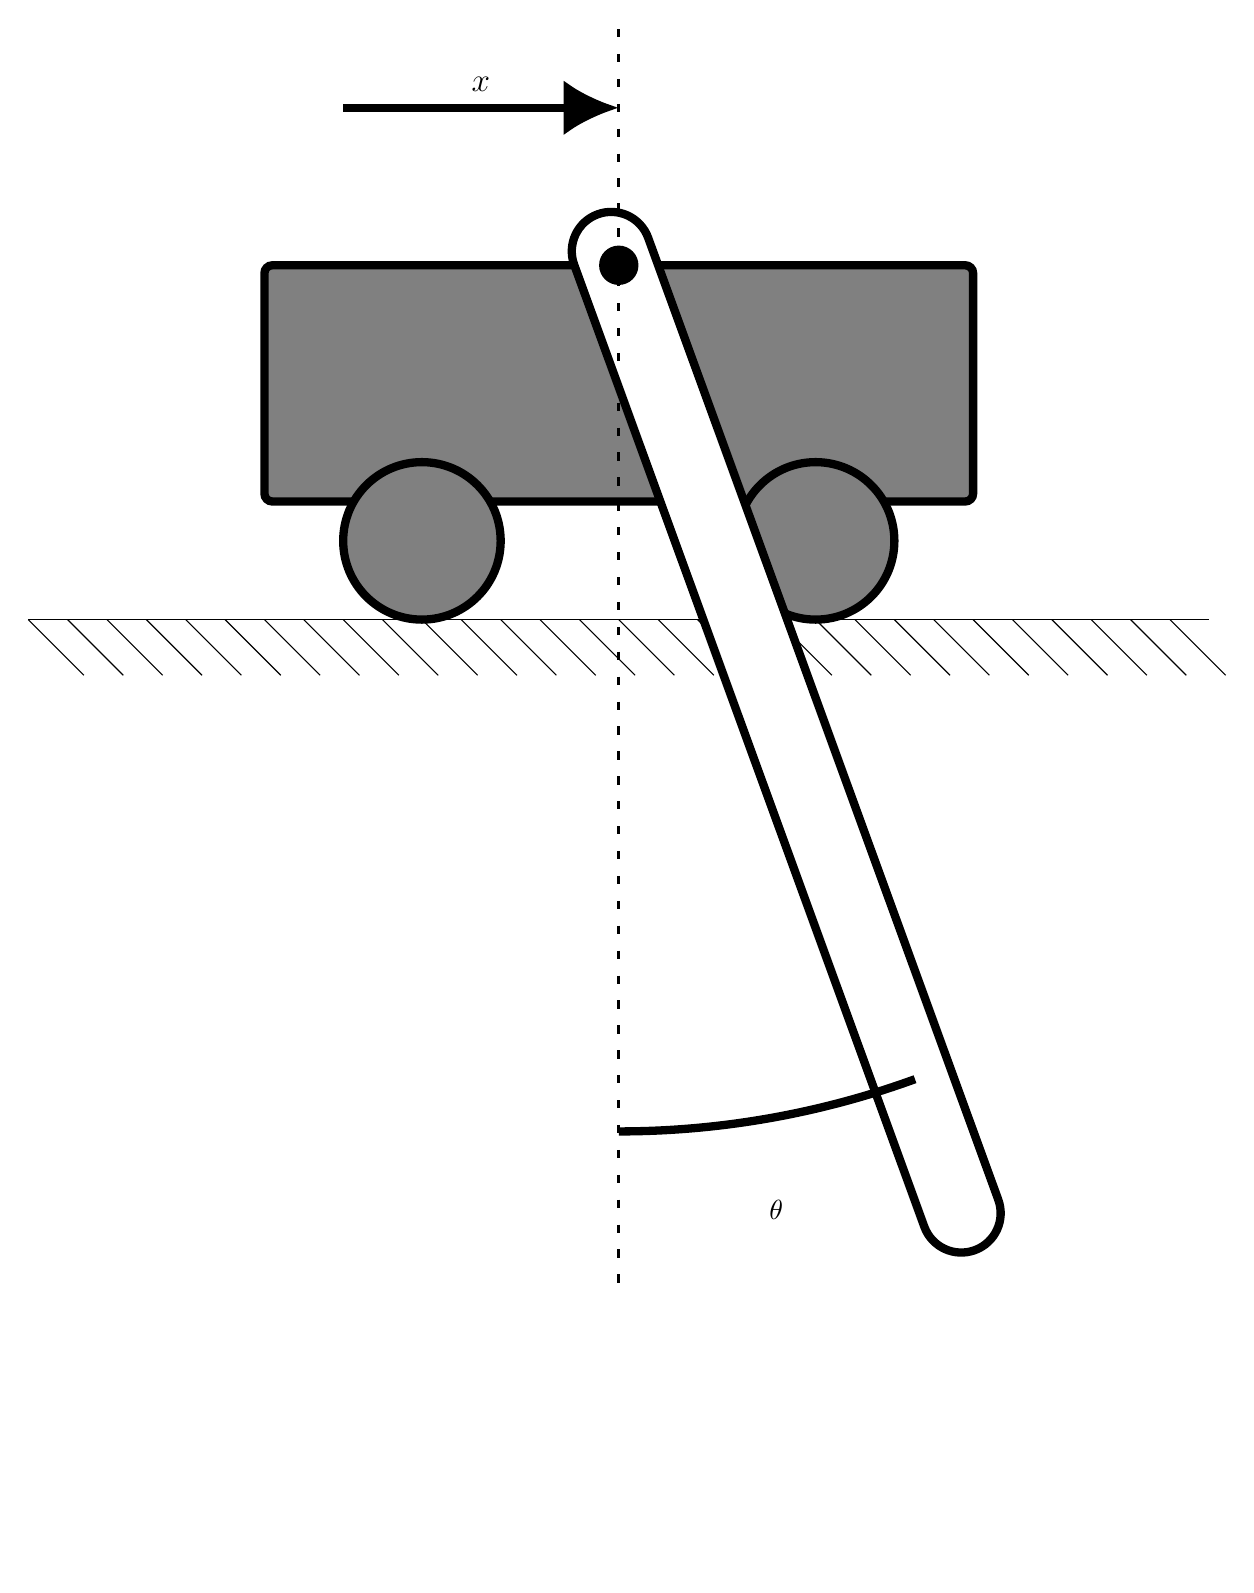
\begin{tikzpicture}[inner sep=0,outer sep=0]
  
    % Draw decorated 'ground'
    \draw[postaction={draw, decorate, decoration={border, angle=-45,
					amplitude=1cm, segment length=.5cm}}] (-3,-1.5) -- (12,-1.5);
  
    % The cart
    \draw[draw=black,fill=black!50,draw=black,line width=3pt,rounded corners=1mm] (0,0) rectangle (9cm,3cm);
    \node[fill=black,circle,minimum size=.5cm] (dot) at (4.5cm,3cm) {};
    
    % Wheels
    \node[fill=white,draw=black,line width=3pt,circle,minimum size=2cm,,fill=black!50] at (2cm,-.5cm) {};
    \node[fill=white,draw=black,line width=3pt,circle,minimum size=2cm,fill=black!50] at (7cm,-.5cm) {};  
    
    % The arm
    \node[anchor=north,minimum width=1cm,minimum height=14cm,draw=black,rotate=20,rounded corners=5mm,yshift=7mm,xshift=-.3mm,fill=white,draw=black,line width=3pt] at (dot) {};
    \node[fill=black,circle,minimum size=.5cm] at (dot) {};
    
    % Markings
    \draw[loosely dashed,line width=1pt] (4.5,6) -- (4.5,-10);
    
    % Arrow
    \draw[->,black,line width=3pt,-{Latex[length=7mm,width=7mm]}] (1,5) --node[above,outer sep=6pt]{\large $x$} (4.5,5);
    
    \def\centerarc[#1](#2)(#3:#4:#5)% Syntax: [draw options] (center) (initial angle:final angle:radius)
    { \draw[#1] ($(#2)+({#5*cos(#3)},{#5*sin(#3)})$) arc (#3:#4:#5); }
    
    % Draw arc
    \centerarc[black,line width=3pt](dot)(270:290:11)
    \node at (6.5,-9) {$\theta$};
    
    \node[white,minimum size=1cm] at (4.5,-13) {};
    
  \end{tikzpicture}}
  \end{subfigure}
  \hfill
  \begin{subfigure}{.78\textwidth}
    \tikz\node[minimum width=\textwidth,minimum height=.35\textwidth,fill=black!10,rounded corners=2pt]{RL trjectories or something interesting?};
  \end{subfigure}
  \hfill
  \caption{Add caption.}
  \label{fig:rl}
\end{figure}




% \begin{figure}
%   \centering
%   \includegraphics[width=0.5\textwidth, angle=270]{fig/weight-space-to-functio-space.pdf}
%   \caption{}
% \end{figure}

% \begin{figure}
%   \centering
%   \includegraphics[width=0.5\textwidth, trim=0 100 0 10]{fig/cartpole-training-curves.pdf}
%   \caption{}
% \end{figure}

% \begin{table}
%   \caption{Negative test log likelihood (lower is better) on UCI classification tasks (2 hidden layers, 50 tanh). Our SVGP predictive outperforms the GLM predictive. }
% \end{table}

\section{Discussion and Conclusion}
\label{sec:conclusion}







A reference implementation of the methods presented in this paper is currently available as supplementary material and will be made available under the MIT License on GitHub upon acceptance.


%\section*{Broader Impact}

% \section*{References}
%\small
%\printbibliography
%\normalsize
% TODO make bibliography small a better way

%References follow the acknowledgments. Use unnumbered first-level heading for
%the references. Any choice of citation style is acceptable as long as you are
%consistent. It is permissible to reduce the font size to \verb+small+ (9 point)
%when listing the references.
%Note that the Reference section does not count towards the page limit.
%\medskip


\phantomsection%
\addcontentsline{toc}{section}{References}
\begingroup
\small
\bibliographystyle{abbrvnat}
\bibliography{zotero-library,bibliography}
\endgroup

\clearpage

\nipstitle{
    {\Large Supplementary Material:} \\
    PAPER TITLE GOES HERE}
\pagestyle{empty}

\appendix

\section{Method Details}

Optionally include extra information (complete proofs, additional experiments and plots) in the appendix.
This section will often be part of the supplemental material.

\section{Model-based Reinforcement Learning with Fast Updates}


\subsection{Problem Statement and Background} \label{sec:problem-statement}
We consider environments with states \(\state \in \stateDomain \), actions \(\action \in \actionDomain\) and transition dynamics \(\transitionFn: \stateDomain \times \actionDomain \rightarrow \stateDomain \) subject to
iid noise \(\noise_{t}\), given by,
\begin{align}
\state_{t+1} = \transitionFn(\state_{t}, \action_{t}) + \noise_{t}.
\end{align}
\begin{assumption}
  (system properties) The environment's dynamics are $L_{\transitionFn}\text{-Lipschitz}$ continuous and the transition noise $\noise_{t}$ is $\sigma\text{-sub-Gaussian}$ for all $t \geq 0$.
\end{assumption}

\subsection{Model-based Reinforcement Learning (RL)}
The goal of reinforcement learning is to find a policy \(\pi \in \Pi\) that maximises the sum of discounted
rewards in expecation under the transition noise (aleatoric uncertainty),
\begin{align} \label{eq-model-free-objective}
\policy^{*} = \arg \max_{\policy \in \policyDomain} J(\transitionFn, \policy) = \arg \max_{\policy \in \policyDomain} \mathbb{E}_{\noise_{0:\infty}} \left[ \sum_{t=0}^{\infty} \discount^{t} \rewardFn(\state_{t},\action_{t}) \right],
\end{align}
where $\gamma \in [0, 1]$

\textbf{Model-based}
In Bayesian model-based RL, we obtain the posterior over the dynamics \(p(f\mid\mathcal{D})\) after performing (approximate) Bayesian
inference given a state transition data set \(\mathcal{D} = \{\{(s_{t},a_{t}), s_{t+1}\}^{T_{i}}_{t=1}\}_{i=0}^{N}\).
\cref{alg-mbrl} shows the typical model-based RL loop.
Importantly, the dynamics are usually only updated after an episode $i$.

\begin{algorithm}[!b]
\caption{Model-based RL}\label{alg-mbrl}
\begin{algorithmic}[1]
  \Require Start state $\state_{0}$, initial data set $\dataset_{0}$, dynamics posterior $p(\transitionFn \mid \dataset_{0})$, policy $\policy_{0}$
\For{$i  \in \{1, 2, \ldots, \text{num episodes} \}$}
    \State Reset the system to $\state_{0}$ and reset trajectory buffers $\bm\tau_{t} = \emptyset \ \forall t$
    \For{$t  \in \{1, 2, \ldots, \text{num steps} \}$}
      % \State Collect  $\tau_{0:t} = \tau_{0:t-1} \cup (\state_{j}, \action_{j}, \state_{j+1}, r_{j+1})$
      \State Use \cref{eq-greedy}/\cref{eq-posterior-sampling}/\cref{eq-ucrl} to collect data $\bm\tau_{t} = \bm\tau_{t-1} \cup (\state_{t}, \policy_{i}(\state_{t}), \transitionFn(\state_{t}, \policy_{i}(\state_{t})), r_{t+1})$
      % \State Execute policy $\policy_{i}(\state_{t})$ in environment and update trajectory $\tau_{i+1} = \{\state_{j}, \action_{j}, \state_{j+1}, r_{j+1}) \}_{j=0}^{t}$
    \EndFor
    \State Update data set $\dataset_{0:i} = \dataset_{0:i-1} \cup \tau$
    \State Train dynamics $p(\transitionFn \mid \dataset_{0:i}) \leftarrow \text{update\_dynamics}(\dataset_{0:i}, p(\transitionFn \mid \dataset_{0:i-1}))$
    % \State Train dynamics $p(\transitionFn \mid \dataset_{0:i+1})$ using $\dataset_{0:i+1}$
    % \State Improve policy $\pi_{i+1}$ using $p(\transitionFn \mid \dataset_{0:i+1})$ and/or $\dataset_{0:i+1}$
    \State Improve policy $\pi_{i+1} \leftarrow \text{update\_policy}(p\left(\transitionFn \mid \dataset_{0:i}), \dataset_{0:i} \right)$
    %\State Improve policy $\pi_{i+1}$ using $p(\transitionFn \mid \dataset_{0:i+1})$ and/or $\dataset_{0:i+1}$
\EndFor
\end{algorithmic}
\end{algorithm}

% \begin{minipage}{0.499\textwidth}
% \begin{algorithm}[H]
% \caption{Model-based RL}\label{alg-mbrl}
% \begin{algorithmic}[1]
%   \Require Initial data set $\dataset_{0}$, dynamics posterior $p(\transitionFn \mid \dataset_{0})$, policy $\policy_{0}$
% \For{$i  \in \{0, 1, \ldots, \text{num episodes} \}$}
%     \For{$t  \in \{0, 1, \ldots, \text{num steps} \}$}
%       \State Execute policy $\policy_{i}(\state_{t})$ in environment
%       \State $\tau_{i+1} = \{\state_{j}, \action_{j}, \state_{j+1}, r_{j+1}) \}_{j=0}^{t}$
%     \EndFor
%     \State Update data set $\mathcal{D}_{0:i+1} = \mathcal{D}_{0:i} \cup \tau_{i+1}$
%     \State Train dynamics $p(\transitionFn \mid \dataset_{0:i+1})$
%     \State Improve policy $\pi_{i+1}$
%     %\State Improve policy $\pi_{i+1}$ using $p(\transitionFn \mid \dataset_{0:i+1})$ and/or $\dataset_{0:i+1}$
% \EndFor
% \end{algorithmic}
% \end{algorithm}
% \end{minipage}
% \hfill
% \begin{minipage}{0.499\textwidth}
% \begin{algorithm}[H]
% \caption{Model-based RL with fast updates}\label{alg-mbrl-fast-updates}
% \begin{algorithmic}[1]
%   \Require Initial data set $\dataset_{0}$, dynamics posterior $p(\transitionFn \mid \dataset_{0})$, policy $\policy_{0}$
%     % ${p(\state_{\timeInd+1} \mid \singleInput, \dataset_{0})}$}
% \For{$i  \in \{0, 1, \ldots, \text{num episodes} \}$}
%     \For{$t  \in \{0, 1, \ldots, \text{num steps} \}$}
%       \State Execute policy $\policy_{i}(\state_{t})$ in environment
%       % \State Append transition $\state_{t}, \action_{t}, \state_{t+1}, r_{t+1})$ to trajectory $\tau_{i}$
%       \State $\tau_{i+1} = \{\state_{j}, \action_{j}, \state_{j+1}, r_{j+1}) \}_{j=0}^{t}$
%       \State {\color{blue}Update dynamics $p(\transitionFn \mid \dataset_{0:i} \cup \tau_{i+1})$}
%     \EndFor
%     \State Update data set $\mathcal{D}_{0:i+1} = \mathcal{D}_{0:i} \cup \tau_{i+1}$
%     \State Train dynamics $p(\transitionFn \mid \dataset_{0:i+1})$
%     \State Improve policy $\pi_{i+1}$
%     %\State Improve policy $\pi_{i+1}$ using $p(\transitionFn \mid \dataset_{0:i+1})$ and/or $\dataset_{0:i+1}$
% \EndFor
% \end{algorithmic}
% \end{algorithm}
% \end{minipage}



\subsection{Exploration Strategies}
\textbf{Greedy exploitation}
Given the posterior dynamics \(p(\transitionFn \mid \mathcal{D})\),
a common approach is to simply take the expecation over both the aleatoric and epistemic uncertainty,
\begin{align} \label{eq-greedy}
\policy_{i+1}^{\text{greedy}} = \arg \max_{\policy \in \policyDomain} \mathbb{E}_{\transitionFn \sim p(\transitionFn \mid \dataset_{0:i})} \left[ J(\transitionFn, \policy) \right],
\end{align}
This approach has been widely adopted, for example, in PILCO, PETS, GP-MPC
\cite{deisenrothPILCO2011,chuaDeepReinforcementLearning2018,kamtheDataEfficient2018}.
This approach helps to alleviate model bias as the posterior ``knows what the model does not know''.
This is because the predictive posterior \(p(f(s_{t},a_{t}) \mid (s_{t},a_{t}),  \mathcal{D} )\) will be (or should be) uncertain when making
predictions far away from the training data.
The expectation considers all possible dynamics models which prevents the policy optimisation from
exploiting innacuracies in the model.
This approach has no guarantees for exploration in the general case.
However, under specific dynamics and reward structures (e.g. PILCO) this objective can achieve sublinear regret.
\todo{need to double check sublinear regret statement. And give a reference}


\textbf{Posterior sampling}
\cite{osbandWhyPosteriorSampling2017,osbandMoreEfficientReinforcement2013}
\begin{align} \label{eq-posterior-sampling}
\policy_{i+1}^{\text{PS}} = \arg \max_{\policy \in \policyDomain} \left[ J(\transitionFn, \policy) \right] \quad \text{s.t. } \transitionFn \sim p(\transitionFn \mid \dataset_{0:i})
\end{align}

\textbf{Hallucinated upper confidence RL}
A more theoretically grounded exploration strategy is UCRL \citep{jakschNearoptimal2010}, which optimises joinly over
policies and models inside the set
\(\mathcal{M} = \{ f \mid | f(s,a) - \mu_{i}(s, a) | \leq \beta_{i} \Sigma_{i}(s, a) \quad \forall s, a \in \mathcal{S} \times \mathcal{A} \}\), representing all statistically plausible
models under the posterior \(p(f(s,a) \mid \mathcal{D}_{0:i} \cup (s,a)) = \mathcal{N}(f(s,a) \mid \mu_{i}(s,a), \Sigma_{i}(s,a))\) at episode \(i\).
This strategy is given by,
\begin{align} \label{eq-ucrl}
\policy_{i+1}^{\text{UCRL}} = \arg \max_{\policy \in \policyDomain} \max_{\transitionFn \in \mathcal{M}} J(\transitionFn, \policy).
\end{align}
This strategy optimises an optimistic policy over the set of plausible dynamics models.
Although this joint optimisation is intractable in general,
\cite{curiEfficient2020} proposed a practical alternative which is detailed in \cref{sec-hucrl}.

\textbf{MPC vs policy learning}
It is worth noting that the strategies in \cref{eq-greedy,eq-posterior-sampling,eq-ucrl} can be used with both model predictive control (MPC)
techniques, such as the cross entoropy method (CEM), and model-free RL techniques, such as soft actor-critic (SAC).


In this work we are interested in how we can use \(p(f \mid \mathcal{D})\) to alleviate some of the issues in model-based RL,
for example, model bias and the exploration-exploitation trade-off.



\todo{show how to get new $\dualParam{1}$ and $\dualParam{2}$ in Train dynamics line of \cref{alg-mbrl-fast-updates}}
\begin{algorithm}[!t]
\caption{Model-based RL with fast updates}\label{alg-mbrl-fast-updates}
\begin{algorithmic}[1]
  \Require Start state $\state_{0}$, initial data set $\dataset_{0}$, dynamics posterior $p(\transitionFn \mid \dataset_{0})$ (inc. dual parameters $\dualParam{1}, \dualParam{2}$), policy $\policy_{0}$
    % ${p(\state_{\timeInd+1} \mid \singleInput, \dataset_{0})}$}
\For{$i  \in \{1, 2, \ldots, \text{num episodes} \}$}
    \State Reset the system to $\state_{0}$ and reset trajectory buffers $\bm\tau_{t} = \emptyset \ \forall t$
    \For{$t  \in \{1, 2, \ldots, \text{num steps} \}$}
      % \State Execute policy $\policy_{i}(\state_{t})$ (\cref{eq-fast-update-mpc}) in environment
      \State Use \cref{eq-fast-update-mpc} to collect data $\bm\tau_{t} = \bm\tau_{t-1} \cup (\state_{t}, \policy_{i}(\state_{t}), \transitionFn(\state_{t}, \policy^{\text{fast}}_{i}(\state_{t})), r_{t+1})$
      % \State Append transition $\state_{t}, \action_{t}, \state_{t+1}, r_{t+1})$ to trajectory $\tau_{i}$
      % \State $\tau_{i+1} = \{\state_{j}, \action_{j}, \state_{j+1}, r_{j+1}) \}_{j=0}^{t}$
      %\State {\color{blue}Update dynamics $p(\transitionFn \mid \dataset_{0:i} \cup \tau_{i+1})$}
      \State {\color{blue}Update dynamics posterior using \cref{eq-dual-update-svgp}, i.e. fast update}
      % \begin{align}
      % \dualParam{1}^{t+1} &\leftarrow \dualParam{1}^{t} +  \nabla_{\meanParam{1}} \mathbb{E}_{q_{\inducingVariable}(\latentFn(\state_{t}, \action_{t}))} \left[ \log p(\state_{t+1} \mid \latentFn(\state_{t}, \action_{t}) ) \right] \\
      % \dualParam{2}^{t+1} &\leftarrow \dualParam{2}^{t} +  \nabla_{\meanParam{2}} \mathbb{E}_{q_{\inducingVariable}(\latentFn(\state_{t}, \action_{t}))}  \left[ \log p(\state_{t+1} \mid \latentFn(\state_{t}, \action_{t}) ) \right]
      % \end{align}}
    \EndFor
    \State Update data set $\dataset_{0:i} = \dataset_{0:i-1} \cup \tau$
    \State Train dynamics $p(\transitionFn \mid \dataset_{0:i}) \leftarrow \text{update\_dynamics}(\dataset_{0:i}, p(\transitionFn \mid \dataset_{0:i-1}))$
    \State Improve policy $\pi^{\text{fast}}_{i+1} \leftarrow \text{update\_policy}(p\left(\transitionFn \mid \dataset_{0:i}), \dataset_{0:i} \right)$
\EndFor
\end{algorithmic}
\end{algorithm}


\subsubsection{Fast updates}


In this section we extend these fast updates to environment's with high dimensional state spaces and large data sets.
% Our method draws on the connection between BNNs and GPs and formulates a function space SVGP posterior given
Our method uses a BNN dynamic model and draws on the connection between BNNs and GPs
\citep{khanApproximate2019} to formulate a function space SVGP posterior,
where we can apply the fast updates from \cref{eq-dual-update-svgp}.
At a high-level, we first use Laplace's approximation to obtain a weight space posterior for our BNN.
We then linearise our BNN around the optimal parameters and interpret it as a GP.
Finally, we formulate a lower rank approximation of this GP posterior (i.e. a SVGP posterior) using inducing variables.
% formulates a function space SVGP posterior by drawing on the connection between BNNs and GPs.


The strategies in \cref{eq-greedy,eq-posterior-sampling,eq-hucrl} do not update the dynamic model during an episode.
A better approach would be to update the posterior at every time step during an episode, for example,
\begin{subequations}
\begin{align} \label{eq-fast-update-mpc}
  \policy_{i+1}^{\text{greedy}}(\state) &= \arg \max_{\action_{0}} \max_{\action_{1:\Horizon}}
\E_{p(\transitionFn \mid \dataset_{0:i})} \left[J^{\Horizon}(\action_{0:\Horizon}, \transitionFn) \right] + \stateValueFn(\state_{\Horizon+1}) \\
  \policy_{i+1}^{\text{PS}}(\state) &= \arg \max_{\action_{0}} \max_{\action_{1:\Horizon}}
J^{\Horizon}(\action_{0:\Horizon}, \transitionFn) + \stateValueFn(\state_{\Horizon+1}) \quad \text{s.t. } \transitionFn \sim p(\transitionFn \mid \dataset_{0:i} \cup \bm\tau_{t}) \\
  \policy_{i+1}^{\text{UCRL}}(\state) &= \arg \max_{\action_{0}} \max_{\action_{1:\Horizon}} \max_{\transitionFn \in \mathcal{M}}
J^{\Horizon}(\action_{0:\Horizon}, \transitionFn) + \stateValueFn(\state_{\Horizon+1}) \quad \text{s.t. } \mathcal{M} = \{\transitionFn(\state_{t},\action_{t}) - \mu_{i,t}(\state_{t},\action_{t}) \leq \beta_{i,t} \Sigma_{i,t}(\state_{t}, \action_{t})\} \\
  \stateValueFn(\state) &= \mathbb{E} \left[ \sum_{t=0}^{\infty}     \discount^{t} \rewardFn(\state_{t},\action_{t}) \mid \state_{0}=\state \right] \label{eq-value-fn}
\end{align}
\end{subequations}
\begin{subequations}
\begin{align} \label{eq-fast-update-mpc-old}
  \policy^{\text{fast}}(\state) = \arg &\max_{\action_{0}} \max_{\action_{1}, \ldots, \action_{\Horizon}}
  \mathbb{E}_{\state_{\horizon} \sim p(\state_{\horizon+1} \mid \transitionFn(\state_{\horizon}, \action_{\horizon}))} \left[ \sum_{\horizon=0}^{\Horizon}     \discount^{\horizon} \rewardFn(\state_{\horizon},\action_{\horizon}) \mid \state_{0}=\state \right] + \discount^{\Horizon+1} \stateValueFn(\state_{\Horizon+1}) \\
  \stateValueFn(\state) &= \mathbb{E} \left[ \sum_{t=0}^{\infty}     \discount^{t} \rewardFn(\state_{t},\action_{t}) \mid \state_{0}=\state \right] \label{eq-fast-update-mpc}
\end{align}
\end{subequations}

\begin{align} \label{}
  \policy(\state) = \arg &\max_{\action_{0}} \max_{\action_{1}, \ldots, \action_{\Horizon}} \max_{\optimisticTransition \in \optimisticTransitionSet}
  \sum_{\horizon=0}^{\Horizon}  \mathbb{E}_{\noise_{\horizon}} \left[  \discount^{\horizon} \rewardFn(\state_{\horizon},\action_{\horizon}) \right] + \discount^{\Horizon+1} \stateValueFn(\state_{\Horizon+1}) \\
  \text{s.t. } \state_{\horizon+1} &= \optimisticTransition(\state_{\horizon}, \action_{\horizon}) + \noise_{\horizon} \\
  \optimisticTransition(\state_{\horizon}, \action_{\horizon}) &=
\optimisticTransitionMean(\state_{\horizon}, \action_{\horizon}) \pm \beta_{i}
\optimisticTransitionCov(\state_{\horizon}, \action_{\horizon})
\end{align}


\section{Assumptions}\label{sec:assumptions}
This section is a draft, possibly contains mistakes
Assumptions on the model required for deriving regret bounds, in the spirit of \cite{curiCombining2021}. \cref{ass:lipschitz-f} and \cref{ass:lipschitz-gp} are copied from \cite{curiCombining2021}, whereas \cref{ass:calibrated} has been modified to accommodate the mean and variance changing during the episode.
\begin{assumption}\label{ass:lipschitz-f}
The true underlying function $f$ is $L_f$-Lipschitz and the elements of the noise vector $w_n$ are $\sigma$-sub-Gaussian.
\end{assumption}
\begin{assumption}[Well-calibrated]\label{ass:calibrated}
Assume that for any $\delta >0$ $\exists$ a set of sequences $\{\beta_{t, i}\}_{t>0, i=0}^{episode_length}$ such that the model mean and variance functions $\mu_{t, i}$, $\sigma_{t, i}$ satisfy for all $(s, a) \in \mathcal{S} \times \mathcal{A}$ the upper bound
\begin{equation}\label{eq:calibrated}
\text{Pr}(\| f(s, a) - \mu_{t, i}(s, a) \| \leq \beta_{t, i}\sigma_{t, i}) \geq 1 - \delta
\end{equation}
\end{assumption}

\begin{assumption}\label{ass:lipschitz-gp}
The mean and variance functions are lipschitz
\end{assumption}
\section{Proof of regret bounds}
This section is a draft, possibly contains mistakes
Plan for the proof:
\begin{itemize}
\item Following Appendix D in \cite{curiCombining2021}, derive a regret bound for the case where the model $\mu_t$ and $\sigma_t$ can be updated within the episode, if assumptions in \cref{sec:assumptions} are satisfied.
\item Show that sparse GPs satisfy \cref{ass:calibrated}
\end{itemize}



\section{Hallucinated Upper Confidence Reinforcement Learning (H-UCRL)} \label{sec-hucrl}
\cite{curiEfficient2020} introduced a tractable approximation which retains some of the theoretical guarantees whilst
being applicable with deep model-based RL.
They introduce a function \(\eta: \mathcal{S} \times \mathcal{A} \rightarrow [-1, 1]^{p}\) which acts as a hallucinated control input.
The strategy is given by,
\begin{align} \label{eq-hucrl}
\pi_i^{\text{UCRL}} = \arg \max_{\policy \in \policyDomain} \max_{\eta(\cdot) \in [-1,1]} J(\transitionFn, \policy) \quad \text{s.t.} \quad \transitionFn = \mu_{i}(\state_{t}, \action_{t}) + \beta_{i} \Sigma_{i}(\state_{t}, \action_{t}) \eta(\state_{t},\action_{t}).
\end{align}
Intuitively, \(\eta(\state,\action) \in [-1,1]\) enables the optimisation to select any dynamics model
\(\transitionFn\) within \(\pm \beta \Sigma_{i}(\state_{t}, \action_{t})\) of the posterior mean \(\mu_{i}(\state_{t}, \action_{t})\).

\section{Laplace Approximation} \label{sec-laplace-approximation}

\textbf{Laplace approximation}
The Laplace approximation \todo{add citation of original paper} constructs a Gaussian approximation of the weight-space posterior $p(\weights \mid \dataset)$
by using a second-order Taylor expansion of $\mathcal{L}$ around $\weights^{*}$.
The posterior approximation is given by,
\begin{align} \label{eq-laplace-approx-weight-space}
  p(\weights \mid \dataset) \approx \mathcal{N} \left( \weights \mid \weights^{*} , \bm\Sigma_{\weights^{*}} \right)
  \quad \text{with} \quad \bm\Sigma_{\weights} =
 - \nabla_{\weights \weights}^{2} \mathcal{L} ( \dataset ; \weights)|_{\weights=\weights^{*}}
\end{align}
That is, it sets the posterior precision to the Hessian of the loss at the optimal parameters $\weights^{*}$.
It is worth noting that computing the Hessian of the loss can be computationally intractable for large networks.
The prior terms are usually trivial, so we focus on the likelihood here.
The Jacobian and Hessian of the log likelihood can be expressed per data point,
\begin{align} \label{eq-jac}
  \nabla_{\weights} \log p(\mathbf{y} \mid \mathbf{f}(\mathbf{x}; \weights)) &= \mathbf{J}(\mathbf{x})^{T} \mathbf{r}(\mathbf{y} ; \mathbf{f}) \\
  \nabla^{2}_{\weights\weights} \log p(\mathbf{y} \mid \mathbf{f}(\mathbf{x}; \weights)) &= \mathbf{H}(\mathbf{x})^{T}
  \mathbf{r}(\mathbf{y};\mathbf{f}) - \mathbf{J}(\mathbf{x})^{T} \bm\Lambda(\mathbf{y};\mathbf{f}) \mathbf{J}(\mathbf{x}),
\label{eq-hess}
\end{align}
through the Jacobian $\mathbf{J} \in \R^{C \times P}$ and Hessian $\mathbf{H} \in \R^{C \times P \times P}$ of the feature extractor $\mathbf{f}(\mathbf{x}; \bm\weights)$,
\begin{align} \label{eq-jac}
[\mathbf{J}(\cdot)]_{ci} = \odv{f_{c}(\cdot ; \weights)}{\weights_{i}}_{\weights=\weights^{*}} \qquad
[\mathbf{H}(\cdot)]_{cij} = \odv{f_{c}(\cdot ; \weights)}{\weights_{i}\weights_{j}}_{\weights=\weights^{*}}
\end{align}
where
$\mathbf{r}(\mathbf{y}; \mathbf{f}) = \nabla_{\mathbf{f}} \log p(\mathbf{y} \mid \mathbf{f})$ can be interpreted as a residual and
$\bm\Lambda(\mathbf{y} ; \mathbf{f}) = \nabla^{2}_{\mathbf{f} \mathbf{f}} \log p(\mathbf{y} \mid \mathbf{f})$
as per-input noise.
Many approximations exist and can be used alongsied our method.
We refer the reader to \cite{daxbergerLaplace2021} for more details.
See \cref{sec-laplace-approximation} for further details on the Laplace approximation.


\section{Experiment details}

\subsection{UCI}

\begin{table}[t!] 
  \centering\scriptsize
  \caption{Negative log predictive density (NLPD) (lower better) for the proposed model TODO} 
	\label{tbl:uci_all}
	% Control table spacing
	\renewcommand{\arraystretch}{1.}
	\setlength{\tabcolsep}{2pt}
	\setlength{\tblw}{0.14\textwidth}  
	
	% Custom error formatting
	\newcommand{\val}[2]{%
		$#1$\textcolor{gray}{\tiny ${\pm}#2$}
	} 

    % THE TABLE NUMBER ARE GENERATED BY A SCRIPT	
	\begin{tabular}{l C{0.6\tblw} C{0.6\tblw} C{0.6\tblw} C{0.6\tblw} C{0.6\tblw} C{0.6\tblw} C{0.6\tblw} C{0.6\tblw} C{0.6\tblw} C{0.6\tblw} C{0.6\tblw} C{0.6\tblw} C{0.6\tblw} C{0.6\tblw}}
\toprule
& SVGP (16) & GP subset(16) & SVGP (32) & GP subset(32) & SVGP (64) & GP subset(64) & SVGP (128) & GP subset(128) & GP all  \\
\midrule
\sc australian & \val{0.322}{0.028} & \val{0.467}{0.02} & \val{0.316}{0.031} & \val{0.406}{0.016} & \val{0.316}{0.03} & \val{0.369}{0.018} & \val{0.316}{0.03} & \val{0.339}{0.025} & \val{0.316}{0.03} \\
\sc cancer & \val{0.102}{0.034} & \val{0.268}{0.012} & \val{0.103}{0.036} & \val{0.206}{0.017} & \val{0.102}{0.036} & \val{0.163}{0.02} & \val{0.102}{0.036} & \val{0.129}{0.027} & \val{0.102}{0.036} \\
\sc ionosphere & \val{0.333}{0.041} & \val{0.486}{0.02} & \val{0.313}{0.046} & \val{0.434}{0.025} & \val{0.306}{0.048} & \val{0.396}{0.032} & \val{0.306}{0.049} & \val{0.341}{0.04} & \val{0.306}{0.049} \\
\sc glass & \val{0.982}{0.072} & \val{1.225}{0.047} & \val{0.886}{0.082} & \val{1.086}{0.073} & \val{0.867}{0.088} & \val{1.007}{0.077} & \val{0.863}{0.091} & \val{0.891}{0.087} & \val{0.861}{0.091} \\
\sc vehicle & \val{0.545}{0.023} & \val{1.001}{0.024} & \val{0.51}{0.021} & \val{0.848}{0.027} & \val{0.478}{0.03} & \val{0.669}{0.015} & \val{0.444}{0.032} & \val{0.578}{0.017} & \val{0.441}{0.035} \\
\sc waveform & \val{0.352}{0.024} & \val{0.651}{0.009} & \val{0.343}{0.025} & \val{0.535}{0.017} & \val{0.339}{0.027} & \val{0.457}{0.017} & \val{0.339}{0.027} & \val{0.392}{0.022} & \val{0.339}{0.027} \\
\sc digits & \val{0.458}{0.017} & \val{1.724}{0.049} & \val{0.375}{0.015} & \val{1.394}{0.01} & \val{0.338}{0.018} & \val{1.088}{0.021} & \val{0.316}{0.018} & \val{0.801}{0.019} & \val{0.083}{0.027} \\
\sc satellite & \val{0.366}{0.014} & \val{1.111}{0.026} & \val{0.32}{0.013} & \val{0.827}{0.016} & \val{0.292}{0.013} & \val{0.632}{0.015} & \val{0.281}{0.013} & \val{0.514}{0.009} & \val{0.256}{0.012} \\
\bottomrule
\end{tabular}

\end{table}

\section{Template stuff}
\subsection{Generate TikZ Figures from Python}
We can generate figures in \texttt{.tex} format directly from Python:
\begin{verbatim}
tikzplotlib.save("fig.tex", axis_width="\\figurewidth", axis_height="\\figureheight")
\end{verbatim}
\cref{fig:example} shows that we get nicely formatted lables/titles/etc when we include them in our paper.
\begin{figure}[h]
    \centering\footnotesize

    % Set your figure size here
    \setlength{\figurewidth}{.33\textwidth}
    \setlength{\figureheight}{.75\figurewidth}

    % Customize your plot here
    % (scale only axis applies the size to the axis box and not entire figure)
    \pgfplotsset{grid style={dotted},title={Foo},scale only axis}

    % Use the subcaption package (= subfigure) for sub-plots, that is
    % plot the separate plots separately in Python
    \begin{subfigure}{.4\textwidth}
        \centering
        % This file was created with tikzplotlib v0.10.1.
\begin{tikzpicture}

\definecolor{darkgray176}{RGB}{176,176,176}
\definecolor{steelblue31119180}{RGB}{31,119,180}

\begin{axis}[
height=\figureheight,
tick align=outside,
tick pos=left,
width=\figurewidth,
x grid style={darkgray176},
xmin=-0.05, xmax=1.05,
xtick style={color=black},
y grid style={darkgray176},
ymin=-0.0420735492403948, ymax=0.883544534048291,
ytick style={color=black}
]
\addplot [semithick, steelblue31119180]
table {%
0 0
0.111111111111111 0.110882628509953
0.222222222222222 0.220397743456122
0.333333333333333 0.327194696796152
0.444444444444444 0.429956363528356
0.555555555555556 0.527415385771866
0.666666666666667 0.618369803069737
0.777777777777778 0.701697876146735
0.888888888888889 0.77637192130066
1 0.841470984807897
};
\end{axis}

\end{tikzpicture}

    \end{subfigure}
    \hfill
    \begin{subfigure}{.4\textwidth}
        \centering
        % This file was created with tikzplotlib v0.10.1.
\begin{tikzpicture}

\definecolor{darkgray176}{RGB}{176,176,176}
\definecolor{steelblue31119180}{RGB}{31,119,180}

\begin{axis}[
height=\figureheight,
tick align=outside,
tick pos=left,
width=\figurewidth,
x grid style={darkgray176},
xmin=-0.05, xmax=1.05,
xtick style={color=black},
y grid style={darkgray176},
ymin=-0.0420735492403948, ymax=0.883544534048291,
ytick style={color=black}
]
\addplot [semithick, steelblue31119180]
table {%
0 0
0.111111111111111 0.110882628509953
0.222222222222222 0.220397743456122
0.333333333333333 0.327194696796152
0.444444444444444 0.429956363528356
0.555555555555556 0.527415385771866
0.666666666666667 0.618369803069737
0.777777777777778 0.701697876146735
0.888888888888889 0.77637192130066
1 0.841470984807897
};
\end{axis}

\end{tikzpicture}

    \end{subfigure}
    \caption{Foo}
    \label{fig:example}
\end{figure}

\subsection{Generate Tables from Python}
We can also generate tables straight from python using \href{https://github.com/astanin/python-tabulate}{tabulate}:
\begin{verbatim}
table = [["Sun",696000,1989100000],["Earth",6371,5973.6],
        ["Moon",1737,73.5],["Mars",3390,641.85]]
headers = ["Planet","R (km)", "mass (x 10^29 kg)"]
table = tabulate(table, headers=headers, tablefmt="latex")
with open("table.tex", 'w') as file:
    file.write(table)
\end{verbatim}

\begin{table}[h]
    \centering
    \begin{tabular}{lrr}
\hline
 Planet   &   R (km) &   mass (x 10\^{}29 kg) \\
\hline
 Sun      &   696000 &          1.9891e+09 \\
 Earth    &     6371 &       5973.6        \\
 Moon     &     1737 &         73.5        \\
 Mars     &     3390 &        641.85       \\
\hline
\end{tabular}
\end{table}

\subsection{Biblatex}
Rember when using biblatex to use 'parencite' for \citep{kamtheDataEfficient2018} and when using natbib to use 'citep'.

%\bibliography{biblio.bib}
\end{document}
